% Options for packages loaded elsewhere
\PassOptionsToPackage{unicode}{hyperref}
\PassOptionsToPackage{hyphens}{url}
%
\documentclass[
  oneside]{book}
\usepackage{amsmath,amssymb}
\usepackage{lmodern}
\usepackage{iftex}
\ifPDFTeX
  \usepackage[T1]{fontenc}
  \usepackage[utf8]{inputenc}
  \usepackage{textcomp} % provide euro and other symbols
\else % if luatex or xetex
  \usepackage{unicode-math}
  \defaultfontfeatures{Scale=MatchLowercase}
  \defaultfontfeatures[\rmfamily]{Ligatures=TeX,Scale=1}
\fi
% Use upquote if available, for straight quotes in verbatim environments
\IfFileExists{upquote.sty}{\usepackage{upquote}}{}
\IfFileExists{microtype.sty}{% use microtype if available
  \usepackage[]{microtype}
  \UseMicrotypeSet[protrusion]{basicmath} % disable protrusion for tt fonts
}{}
\makeatletter
\@ifundefined{KOMAClassName}{% if non-KOMA class
  \IfFileExists{parskip.sty}{%
    \usepackage{parskip}
  }{% else
    \setlength{\parindent}{0pt}
    \setlength{\parskip}{6pt plus 2pt minus 1pt}}
}{% if KOMA class
  \KOMAoptions{parskip=half}}
\makeatother
\usepackage{xcolor}
\IfFileExists{xurl.sty}{\usepackage{xurl}}{} % add URL line breaks if available
\IfFileExists{bookmark.sty}{\usepackage{bookmark}}{\usepackage{hyperref}}
\hypersetup{
  pdftitle={Data Skills},
  pdfauthor={Heather Cleland-Woods and Emily Nordmann},
  hidelinks,
  pdfcreator={LaTeX via pandoc}}
\urlstyle{same} % disable monospaced font for URLs
\usepackage[margin=1in]{geometry}
\usepackage{color}
\usepackage{fancyvrb}
\newcommand{\VerbBar}{|}
\newcommand{\VERB}{\Verb[commandchars=\\\{\}]}
\DefineVerbatimEnvironment{Highlighting}{Verbatim}{commandchars=\\\{\}}
% Add ',fontsize=\small' for more characters per line
\usepackage{framed}
\definecolor{shadecolor}{RGB}{248,248,248}
\newenvironment{Shaded}{\begin{snugshade}}{\end{snugshade}}
\newcommand{\AlertTok}[1]{\textcolor[rgb]{0.94,0.16,0.16}{#1}}
\newcommand{\AnnotationTok}[1]{\textcolor[rgb]{0.56,0.35,0.01}{\textbf{\textit{#1}}}}
\newcommand{\AttributeTok}[1]{\textcolor[rgb]{0.77,0.63,0.00}{#1}}
\newcommand{\BaseNTok}[1]{\textcolor[rgb]{0.00,0.00,0.81}{#1}}
\newcommand{\BuiltInTok}[1]{#1}
\newcommand{\CharTok}[1]{\textcolor[rgb]{0.31,0.60,0.02}{#1}}
\newcommand{\CommentTok}[1]{\textcolor[rgb]{0.56,0.35,0.01}{\textit{#1}}}
\newcommand{\CommentVarTok}[1]{\textcolor[rgb]{0.56,0.35,0.01}{\textbf{\textit{#1}}}}
\newcommand{\ConstantTok}[1]{\textcolor[rgb]{0.00,0.00,0.00}{#1}}
\newcommand{\ControlFlowTok}[1]{\textcolor[rgb]{0.13,0.29,0.53}{\textbf{#1}}}
\newcommand{\DataTypeTok}[1]{\textcolor[rgb]{0.13,0.29,0.53}{#1}}
\newcommand{\DecValTok}[1]{\textcolor[rgb]{0.00,0.00,0.81}{#1}}
\newcommand{\DocumentationTok}[1]{\textcolor[rgb]{0.56,0.35,0.01}{\textbf{\textit{#1}}}}
\newcommand{\ErrorTok}[1]{\textcolor[rgb]{0.64,0.00,0.00}{\textbf{#1}}}
\newcommand{\ExtensionTok}[1]{#1}
\newcommand{\FloatTok}[1]{\textcolor[rgb]{0.00,0.00,0.81}{#1}}
\newcommand{\FunctionTok}[1]{\textcolor[rgb]{0.00,0.00,0.00}{#1}}
\newcommand{\ImportTok}[1]{#1}
\newcommand{\InformationTok}[1]{\textcolor[rgb]{0.56,0.35,0.01}{\textbf{\textit{#1}}}}
\newcommand{\KeywordTok}[1]{\textcolor[rgb]{0.13,0.29,0.53}{\textbf{#1}}}
\newcommand{\NormalTok}[1]{#1}
\newcommand{\OperatorTok}[1]{\textcolor[rgb]{0.81,0.36,0.00}{\textbf{#1}}}
\newcommand{\OtherTok}[1]{\textcolor[rgb]{0.56,0.35,0.01}{#1}}
\newcommand{\PreprocessorTok}[1]{\textcolor[rgb]{0.56,0.35,0.01}{\textit{#1}}}
\newcommand{\RegionMarkerTok}[1]{#1}
\newcommand{\SpecialCharTok}[1]{\textcolor[rgb]{0.00,0.00,0.00}{#1}}
\newcommand{\SpecialStringTok}[1]{\textcolor[rgb]{0.31,0.60,0.02}{#1}}
\newcommand{\StringTok}[1]{\textcolor[rgb]{0.31,0.60,0.02}{#1}}
\newcommand{\VariableTok}[1]{\textcolor[rgb]{0.00,0.00,0.00}{#1}}
\newcommand{\VerbatimStringTok}[1]{\textcolor[rgb]{0.31,0.60,0.02}{#1}}
\newcommand{\WarningTok}[1]{\textcolor[rgb]{0.56,0.35,0.01}{\textbf{\textit{#1}}}}
\usepackage{longtable,booktabs,array}
\usepackage{calc} % for calculating minipage widths
% Correct order of tables after \paragraph or \subparagraph
\usepackage{etoolbox}
\makeatletter
\patchcmd\longtable{\par}{\if@noskipsec\mbox{}\fi\par}{}{}
\makeatother
% Allow footnotes in longtable head/foot
\IfFileExists{footnotehyper.sty}{\usepackage{footnotehyper}}{\usepackage{footnote}}
\makesavenoteenv{longtable}
\usepackage{graphicx}
\makeatletter
\def\maxwidth{\ifdim\Gin@nat@width>\linewidth\linewidth\else\Gin@nat@width\fi}
\def\maxheight{\ifdim\Gin@nat@height>\textheight\textheight\else\Gin@nat@height\fi}
\makeatother
% Scale images if necessary, so that they will not overflow the page
% margins by default, and it is still possible to overwrite the defaults
% using explicit options in \includegraphics[width, height, ...]{}
\setkeys{Gin}{width=\maxwidth,height=\maxheight,keepaspectratio}
% Set default figure placement to htbp
\makeatletter
\def\fps@figure{htbp}
\makeatother
\setlength{\emergencystretch}{3em} % prevent overfull lines
\providecommand{\tightlist}{%
  \setlength{\itemsep}{0pt}\setlength{\parskip}{0pt}}
\setcounter{secnumdepth}{5}
\usepackage{booktabs}

\usepackage{tcolorbox}
\usepackage[T1]{fontenc}

\definecolor{dangcol}{RGB}{152,62,130}
\definecolor{warncol}{RGB}{245,220,112}
\definecolor{infocol}{RGB}{70,122,172}
\definecolor{trycol}{RGB}{97,88,156}

\newtcolorbox{dangerous}{
  colback=dangcol!10,
  colframe=dangcol,
  coltext=black,
  boxsep=5pt,
  arc=4pt
}

\newtcolorbox{warning}{
  colback=warncol!10,
  colframe=warncol,
  coltext=black,
  boxsep=5pt,
  arc=4pt
}

\newtcolorbox{info}{
  colback=infocol!10,
  colframe=infocol,
  coltext=black,
  boxsep=5pt,
  arc=4pt
}

\newtcolorbox{try}{
  colback=trycol!10,
  colframe=trycol,
  coltext=black,
  boxsep=5pt,
  arc=4pt
}
\ifLuaTeX
  \usepackage{selnolig}  % disable illegal ligatures
\fi
\usepackage[]{natbib}
\bibliographystyle{plainnat}

\title{Data Skills}
\author{Heather Cleland-Woods and Emily Nordmann}
\date{2021-09-18}

\begin{document}
\maketitle

{
\setcounter{tocdepth}{1}
\tableofcontents
}
\hypertarget{overview}{%
\chapter*{Overview}\label{overview}}
\addcontentsline{toc}{chapter}{Overview}

By the end of this book, you will be able to:

\begin{itemize}
\tightlist
\item
  Import data into R
\item
  Manipulate and wrangle data into an appropriate format for analysis
\item
  Calculate summarises of descriptive statistics
\item
  Produce informative data visualisations
\item
  Perform basic probability calculations using simulation
\end{itemize}

\hypertarget{how-to-use-this-book-and-the-walkthrough-videos}{%
\section{How to use this book and the walkthrough videos}\label{how-to-use-this-book-and-the-walkthrough-videos}}

For most chapters of this book there is an associated walkthrough video. These videos are there to support you as you get comfortable using R, however, it's important that you use them wisely. You should always try to work through each chapter of this book (or if you prefer each activity) on your own and only then watch the video if you get stuck, or for extra information.

For many of the initial chapters, we will provide the code you need to use. You can copy and paste from the book, however, we strongly encourage you to type out the code by yourself. This will seem much slower and you will make errors, but you will learn much more quickly this way.

Additionally, we also provide the solutions to many of the activities. No-one is going to check whether you tried to figure it out yourself rather than going straight to the solution but remember this: if you copy and paste without thinking, you will learn nothing.

Finally, on occasion we will make updates to the book such as fixing typos and including additional detail or activities and as such this book should be considered a living document. When substantial changes are made, new walkthrough videos will be recorded, however, it would be impossible to record a new video every time we made a minor change, therefore, sometimes there may be slight differences between the walkthrough videos and the content of this book. Where there are differences between the book and the video, the book should always be considered the definitive version.

\hypertarget{getting-to-know-the-data}{%
\chapter{Getting to know the data}\label{getting-to-know-the-data}}

This semester we will use the same dataset each week to develop your skills and knowledge. The dataset is from Woodworth et al.~(2018) and you can find an explanation of the data here Web-based Positive Psychology Interventions: A Reexamination of Effectiveness.

There is a \href{https://moodle.gla.ac.uk/filter/echo360/lti_launch.php?url=https\%3A\%2F\%2Fecho360.org.uk\%2Flti\%2F73750256-551c-47b5-9f1b-247567d647c2\%3FmediaId\%3Db75d33c3-4c7b-4586-b019-ee715f169409\%26autoplay\%3Dfalse\%26automute\%3Dfalse\&cmid=2529962\&width=640\&height=420}{walkthrough video} of this chapter available via Echo360 (UofG Moodle sign-in required).

\hypertarget{activity-1}{%
\section{Activity 1}\label{activity-1}}

Read through the study to familiarise yourself with the data you will be using over the coming weeks and answer the below questions.

When you get the correct answer, the answer box will turn green. Sometimes this doesn't work on Internet Explorer or Edge so be sure to use Chrome or Firefox.

\begin{itemize}
\tightlist
\item
  What does the AHI measure? (Hint, use a single word)
\end{itemize}

\begin{itemize}
\tightlist
\item
  What does the CES-D measure? (hint, use a single word)
\end{itemize}

\begin{itemize}
\tightlist
\item
  How many participants were there in this study?
\end{itemize}

\begin{itemize}
\tightlist
\item
  How many questions (items) are there on the AHI?
\end{itemize}

\begin{itemize}
\tightlist
\item
  How many questions (items) are there on the CES-D?
\end{itemize}

\hypertarget{activity-2}{%
\section{Activity 2}\label{activity-2}}

Download the files for Psych 1A here

The files are stored in a \textbf{zip file}. A zip file is a folder that contains files that have been compressed to make the file size smaller (like vacuum packed food) and enables you to download multiple files at once, however, before you use the files from a zip folder you first need to extract them.

\begin{enumerate}
\def\labelenumi{\arabic{enumi}.}
\tightlist
\item
  If you haven't already, make a folder on your computer for Psych 1A.
\item
  Click on the above link to download the folder and save it in your Psych 1A folder. If your computer does not ask you where to save the file, chances are it has saved it in your Downloads folder. If this is the case, once it has downloaded go to your downloads folder and then move it to your Psych 1A folder
\item
  Navigate to the zip file and open it. You will see all the files it contains but \textbf{don't use these} - click \textbf{``Extract all''} on the top ribbon. If you are using and Mac and Safari, you may find that it automatically unzips the folder. This can actually cause more problems than it solves and I would recommend \href{https://apple.stackexchange.com/questions/961/how-to-stop-safari-from-unzipping-files-after-download}{turning it off} but also, Safari sometimes causes other issues with downloading some file types so if you're on a Mac, I really would just use Chrome or Firefox.
\item
  You will be asked to select a location to save the unzipped files. Assuming that you followed step 2, the default option should be your Psych 1A folder
\item
  You can now use the unzipped files. Save the zip folder for now, we're going to use it again in chapter 3.
\end{enumerate}

\hypertarget{activity-3}{%
\section{Activity 3}\label{activity-3}}

Now that you've unzipped the folder, you should see that you have eight files. Three of these files are the data from Woodworth et al.~- \texttt{code-book.pdf}, \texttt{ahi-cesd.csv} and \texttt{participant-info.csv}. Open and review each of these files and use the code book to figure out what the data in each variable (column) represents.

\begin{itemize}
\tightlist
\item
  How many variables/columns data does \texttt{participant-info.csv} have?
\end{itemize}

\begin{itemize}
\tightlist
\item
  How many variables/columns data does \texttt{ahi-cesd.csv} have?
\end{itemize}

\begin{itemize}
\tightlist
\item
  What does a response of 1 for sex mean? femalemale
\end{itemize}

The remaining five files are ``stub files'' that you will use as you work through this book, so don't worry about them just now.

\hypertarget{programming-basics}{%
\chapter{Programming basics}\label{programming-basics}}

In this chapter, we will cover how to use R and RStudio at the University of Glasgow as well as some basic programming concepts and terminology, common pitfalls, helpful hints, and where to get help. Those of you who have no programming experience should find this chapter particularly helpful, however, even if you've used R before there may be some helpful hints and tips so please make sure you read through this chapter before the moving on.

This is a long chapter but we don't expect you to memorise all the information that is contained in it and some sections of it will not make sense until you start writing your own code - just make sure you know what help is available!

There is a \href{https://uofglasgow.zoom.us/rec/play/z4QocMWQL9ExSfHYBaC8C1oISbrEDkOlz8wJwT0oT2y116hgB0yA0O9cTtVdvYWYqO-wq97Xi8_yncLv.1st2ENKayHb21h0S?autoplay=true\&startTime=1600084596000}{walkthrough video} of this chapter available via Zoom.

\hypertarget{r-and-rstudio}{%
\section{R and RStudio}\label{r-and-rstudio}}

R is a programming language that you will write code in and RStudio is an Integrated Development Environment (IDE) which makes working with R easier. Think of it as knowing English and using a plain text editor like NotePad to write a book versus using a word processor like Microsoft Word. You could do it, but it wouldn't look as good and it would be much harder without things like spell-checking and formatting. In a similar way, you can use R without R Studio but we wouldn't recommend it. The key thing to remember is that although you will do all of your work using RStudio for this course, you are actually using two pieces of software which means that from time-to-time, both of them may have separate updates.

There are two ways you can use R for psychology. First, you can use a online version of R and R through your web browser and we will refer to this as the \textbf{R server}. Second, you can download and install R and RStudio for free on your laptop or desktop computer.

\textbf{Which version of R should you use?}

The advantage of using the R server is that you do not need to install anything on your machine, you simply access it through your web browser. All the extra packages and functions you need for this course will already be installed. We recommend using the server if you have a computer that you cannot install R on (e.g., a Chromebook), or if you have serious problems with installing R on your computer.

The advantage to installing R on your computer is that you do not need to be connected to the internet to use it, it is easier to save and manage your files, and there are no problems caused if the server crashes (which is rare, but does and has happened).

With the exception of how they save files, both versions are largely identical in how they work, however, after over a year working remotely, we have concluded that \textbf{if you can install R on your computer, you should}. If your computer cannot install R, or if you have technical problems during the installation you cannot resolve, then you should use the server. However, the need to be connected to the internet and the inability to open e.g., assessment files directly on your computer if you use the server mean that it is worth trying to install it if you can.

\hypertarget{r-server}{%
\subsection{R server}\label{r-server}}

You will find the link to the R server on Moodle. Please note that the R server is only for use by students and staff in the School of Psychology and Neuroscience. Sign in to the R server with your usual GUID and password.

\hypertarget{installing-r-on-your-computer}{%
\subsection{Installing R on your computer}\label{installing-r-on-your-computer}}

To use R on your computer, please see \href{https://psyteachr.github.io/ug1-practical/installing-r.html}{Installing R} which has more detailed instructions and links to the files you need to download, as well as a links to a series of walkthroughs for installing R on different types of computers.

\hypertarget{getting-to-know-r-studio}{%
\section{Getting to know R Studio}\label{getting-to-know-r-studio}}

R Studio has a console that you can try out code in (appearing as the bottom left window in Figure \ref{fig:img-rstudio}), there is a script editor (top left), a window showing functions and objects you have created in the ``Environment'' tab (top right window in the figure), and a window that shows plots, files packages, and help documentation (bottom right).

\begin{figure}

{\centering \includegraphics[width=1\linewidth]{images/rstudio} 

}

\caption{RStudio interface}\label{fig:img-rstudio}
\end{figure}

You will learn more about how to use the features included in R Studio throughout this course, however, we highly recommend watching \href{https://rstudio.com/resources/webinars/programming-part-1-writing-code-in-rstudio/}{RStudio Essentials 1} from the R Studio team. The video lasts \textasciitilde30 minutes and gives a tour of the main parts of R Studio.

\hypertarget{console-vs.-scripts}{%
\section{Console vs.~scripts}\label{console-vs.-scripts}}

When you first open up R Studio you won't see a script like above, there will just be a single pane on the left, which is the console. You can write code in the console to test it out, but it won't save anywhere. For this chapter, we'll use the console to show you some simple code examples but moving forward you'll save your code in a script file, and you'll see the extra pane appear.

\hypertarget{functions-and-arguments}{%
\section{Functions and arguments}\label{functions-and-arguments}}

\textbf{Functions} in R execute specific tasks and normally take a number of \textbf{arguments} (if you're into linguistics you might want to think as these as verbs that require a subject and an object). You can look up all the arguments that a function takes by using the help documentation by using the format \texttt{?function}. Some arguments are required, and some are optional. Optional arguments will often use a default (normally specified in the help documentation) if you do not enter any value.

As an example, let's look at the help documentation for the function \texttt{rnorm()} which randomly generates a set of numbers with a normal distribution.

\hypertarget{activity-1-1}{%
\section{Activity 1}\label{activity-1-1}}

\begin{itemize}
\tightlist
\item
  Open up R Studio (either on the server or on your machine) and in the console, type the following code:
\end{itemize}

\begin{Shaded}
\begin{Highlighting}[]
\NormalTok{?rnorm}
\end{Highlighting}
\end{Shaded}

The help documentation for \texttt{rnorm()} should appear in the bottom right help panel. In the usage section, we see that \texttt{rnorm()} takes the following form:

\begin{Shaded}
\begin{Highlighting}[]
\FunctionTok{rnorm}\NormalTok{(n, }\AttributeTok{mean =} \DecValTok{0}\NormalTok{, }\AttributeTok{sd =} \DecValTok{1}\NormalTok{)}
\end{Highlighting}
\end{Shaded}

In the arguments section, there are explanations for each of the arguments. \texttt{n} is the number of observations we want to create, \texttt{mean} is the mean of the data points we will create and \texttt{sd} is the standard deviation of the set. In the details section it notes that if no values are entered for \texttt{mean} and \texttt{sd} it will use a default of 0 and 1 for these values. Because there is no default value for \texttt{n} it must be specified otherwise the code won't run.

Let's try an example and just change the required argument \texttt{n} to ask R to produce 5 random numbers.

\hypertarget{activity-2-1}{%
\section{Activity 2}\label{activity-2-1}}

\begin{itemize}
\tightlist
\item
  Copy and paste the following code into the console.
\end{itemize}

\begin{Shaded}
\begin{Highlighting}[]
\FunctionTok{set.seed}\NormalTok{(}\DecValTok{12042016}\NormalTok{)}
\FunctionTok{rnorm}\NormalTok{(}\AttributeTok{n =} \DecValTok{5}\NormalTok{)}
\end{Highlighting}
\end{Shaded}

\begin{verbatim}
## [1] -0.2896163 -0.6428964  0.5829221 -0.3286728 -0.5110101
\end{verbatim}

These numbers have a mean of 0 and an SD of 1. Now we can change the additional arguments to produce a different set of numbers.

\begin{Shaded}
\begin{Highlighting}[]
\FunctionTok{rnorm}\NormalTok{(}\AttributeTok{n =} \DecValTok{5}\NormalTok{, }\AttributeTok{mean =} \DecValTok{10}\NormalTok{, }\AttributeTok{sd =} \DecValTok{2}\NormalTok{)}
\end{Highlighting}
\end{Shaded}

\begin{verbatim}
## [1] 13.320853  9.377956 10.235461  9.811793 13.019102
\end{verbatim}

This time R has still produced 5 random numbers, but now this set of numbers has a mean of 10 and an sd of 2 as specified. Always remember to use the help documentation to help you understand what arguments a function requires.

\begin{info}
If you're looking up examples of code online, you may often see code
that starts with the function \texttt{set.seed()}. This function
controls the random number generator - if you're using any functions
that generate numbers randomly (such as \texttt{rnorm()}), running
\texttt{set.seed()} will ensure that you get the same result (in some
cases this may not be what you want to do). We call \texttt{set.seed()}
in this example because it means that you will get the same random
numbers as this book.
\end{info}

\hypertarget{argument-names}{%
\section{Argument names}\label{argument-names}}

In the above examples, we have written out the argument names in our code (e.g., \texttt{n}, \texttt{mean}, \texttt{sd}), however, this is not strictly necessary. The following two lines of code would both produce the same result (although each time you run \texttt{rnorm()} it will produce a slightly different set of numbers, because it's random, but they would still have the same mean and SD):

\begin{Shaded}
\begin{Highlighting}[]
\FunctionTok{rnorm}\NormalTok{(}\AttributeTok{n =} \DecValTok{6}\NormalTok{, }\AttributeTok{mean =} \DecValTok{3}\NormalTok{, }\AttributeTok{sd =} \DecValTok{1}\NormalTok{)}
\FunctionTok{rnorm}\NormalTok{(}\DecValTok{6}\NormalTok{, }\DecValTok{3}\NormalTok{, }\DecValTok{1}\NormalTok{)}
\end{Highlighting}
\end{Shaded}

Importantly, if you do not write out the argument names, R will use the default order of arguments, that is for \texttt{rnorm} it will assume that the first number you enter is \texttt{n}. the second number is \texttt{mean} and the third number is \texttt{sd}.

If you write out the argument names then you can write the arguments in whatever order you like:

\begin{Shaded}
\begin{Highlighting}[]
\FunctionTok{rnorm}\NormalTok{(}\AttributeTok{sd =} \DecValTok{1}\NormalTok{, }\AttributeTok{n =} \DecValTok{6}\NormalTok{, }\AttributeTok{mean =} \DecValTok{3}\NormalTok{)}
\end{Highlighting}
\end{Shaded}

When you are first learning R, you may find it useful to write out the argument names as it can help you remember and understand what each part of the function is doing. However, as your skills progress you may find it quicker to omit the argument names and you will also see examples of code online that do not use argument names so it is important to be able to understand which argument each bit of code is referring to (or look up the help documentation to check).

In this course, we will always write out the argument names the first time we use each function, however, in subsequent uses they may be omitted.

\hypertarget{tab-auto-complete}{%
\section{Tab auto-complete}\label{tab-auto-complete}}

One very useful feature of R Studio is the tab auto-complete for functions (see Figure \ref{fig:img-autocomplete}). If you write the name of the function and then press the tab key, R Studio will show you the arguments that function takes along with a brief description. If you press enter on the argument name it will fill in the name for you, just like auto-complete on your phone. This is incredibly useful when you are first learning R and you should remember to use this feature frequently.

\begin{figure}

{\centering 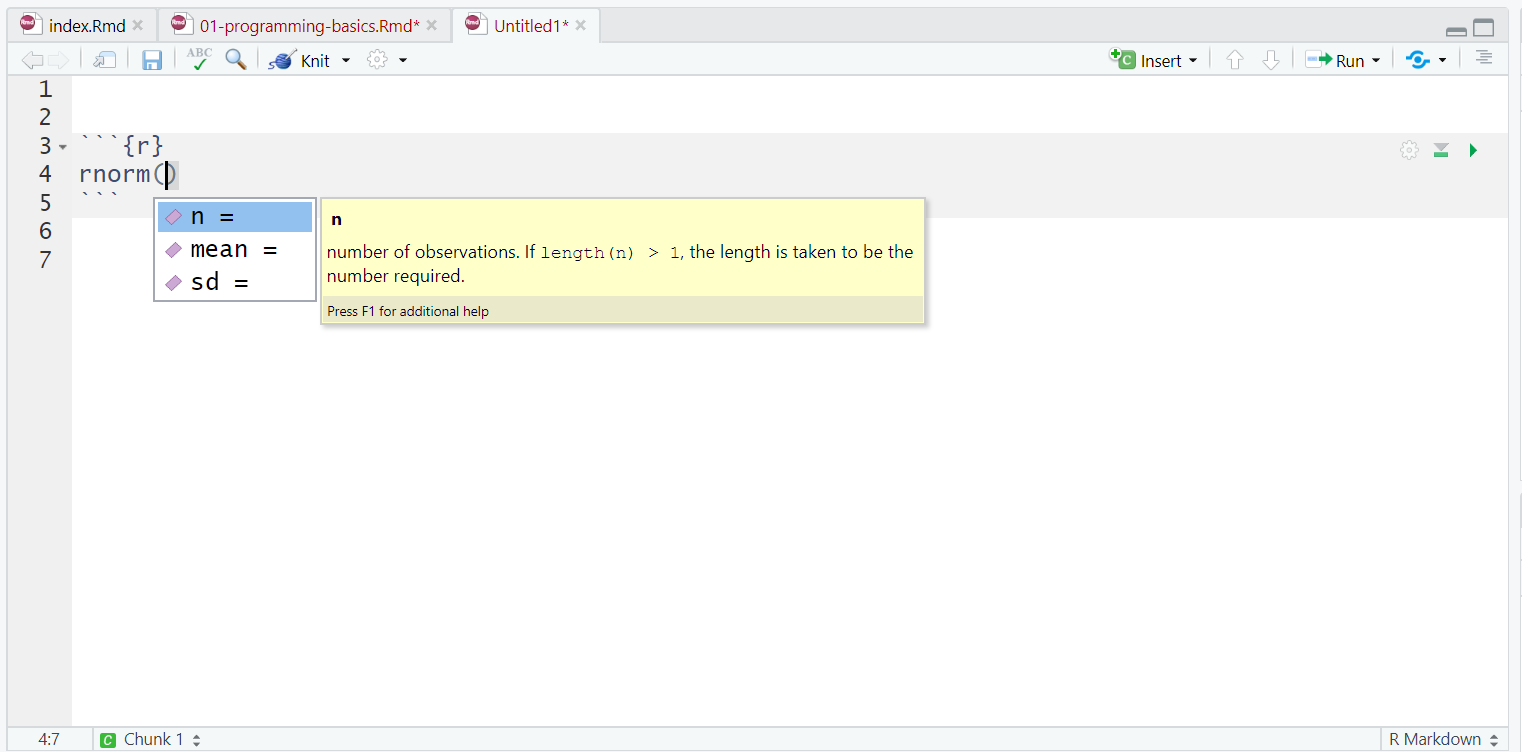
\includegraphics[width=1\linewidth]{images/autocomplete} 

}

\caption{Tab auto-complete}\label{fig:img-autocomplete}
\end{figure}

\hypertarget{packages}{%
\section{Base R and packages}\label{packages}}

When you install R you will have access to a range of functions including options for data wrangling and statistical analysis. The functions that are included in the default installation are typically referred to as \textbf{Base R} and there is a useful cheat sheet that shows many Base R functions \href{https://www.rstudio.com/wp-content/uploads/2016/05/base-r.pdf}{here}.

However, the power of R is that it is extendable and open source - put simply, if a function doesn't exist or doesn't work very well, anyone can create a new \textbf{package} that contains data and code to allow you to perform new tasks. You may find it useful to think of Base R as the default apps that come on your phone and packages as additional apps that you need to download separately.

\hypertarget{activity-3-install-the-tidyverse-optional}{%
\section{Activity 3: Install the tidyverse (optional)}\label{activity-3-install-the-tidyverse-optional}}

In order to use a package, you must first install it. The following code installs the package \texttt{tidyverse}, a package we will use very frequently in this course.

\begin{itemize}
\tightlist
\item
  If you are working on your own computer, use the below code to install the tidyverse. \textbf{You do not need to do this if you are working on the server or if you are using the computers in the Boyd Orr building}.
\end{itemize}

\begin{Shaded}
\begin{Highlighting}[]
\FunctionTok{install.packages}\NormalTok{(}\StringTok{"tidyverse"}\NormalTok{)}
\end{Highlighting}
\end{Shaded}

You only need to install a package once, however, each time you start R you need to load the packages you want to use, in a similar way that you need to install an app on your phone once, but you need to open it every time you want to use it.

\begin{danger}
If you get an error message that says something like ``WARNING: Rtools
is required to build R packages'' you may need to download and install
an extra bit of software called
\href{https://cran.r-project.org/bin/windows/Rtools/}{Rtools}.
\end{danger}

To load packages we use the function \texttt{library()}. Typically you would start any analysis script by loading all of the packages you need, but we will come back to that in the next chapter.

\hypertarget{activity-4-load-the-tidyverse}{%
\section{Activity 4: Load the tidyverse}\label{activity-4-load-the-tidyverse}}

\begin{itemize}
\tightlist
\item
  Run the below code to load the tidyverse. You can do this regardless of whether you are using your own computer or the server.
\end{itemize}

\begin{Shaded}
\begin{Highlighting}[]
\FunctionTok{library}\NormalTok{(tidyverse)}
\end{Highlighting}
\end{Shaded}

You will get what looks like an error message - it's not. It's just R telling you what it's done.

Now that we've loaded the \texttt{tidyverse} package we can use any of the functions it contains but remember, you need to run the \texttt{library()} function every time you start R.

\hypertarget{package-updates}{%
\section{Package updates}\label{package-updates}}

In addition to updates to R and R Studio, the creators of packages also sometimes update their code. This can be to add functions to a package, or it can be to fix errors. One thing to avoid is unintentionally updating an installed package. When you run \texttt{install.packages()} it will always install the latest version of the package and it will overwrite any older versions you may have installed. Sometimes this isn't a problem, however, sometimes you will find that the update means your code no longer works as the package has changed substantially. It is possible to revert back to an older version of a package but try to avoid this anyway.

\begin{danger}
To avoid accidentally overwriting a package with a later version, you
should \textbf{never} include \texttt{install.packages()} in your
analysis scripts in case you, or someone else runs the code by mistake.
Remember, the server will already have all of the packages you need for
this course so you only need to install packages if you are using your
own machine.
\end{danger}

\hypertarget{conflicts}{%
\section{Package conflicts}\label{conflicts}}

There are thousands of different R packages with even more functions. Unfortunately, sometimes different packages have the same function names. For example, the packages \texttt{dplyr} and \texttt{MASS} both have a function named \texttt{select()}. If you load both of these packages, R will produce a warning telling you that there is a conflict.

\begin{Shaded}
\begin{Highlighting}[]
\FunctionTok{library}\NormalTok{(dplyr)}
\FunctionTok{library}\NormalTok{(MASS)}
\end{Highlighting}
\end{Shaded}

\begin{verbatim}
## 
## Attaching package: 'MASS'
\end{verbatim}

\begin{verbatim}
## The following object is masked from 'package:dplyr':
## 
##     select
\end{verbatim}

In this case, R is telling you that the function \texttt{select()} in the \texttt{dplyr} package is being hidden (or `masked') by another function with the same name. If you were to try and use \texttt{select()}, R would use the function from the package that was loaded most recently - in this case it would use the function from \texttt{MASS}.

If you want to specify which package you want to use for a particular function you can use code in the format \texttt{package::function}, for example:

\begin{Shaded}
\begin{Highlighting}[]
\NormalTok{dplyr}\SpecialCharTok{::}\FunctionTok{select}\NormalTok{()}
\NormalTok{MASS}\SpecialCharTok{::}\FunctionTok{select}\NormalTok{()}
\end{Highlighting}
\end{Shaded}

\hypertarget{objects}{%
\section{Objects}\label{objects}}

A large part of your coding will involve creating and manipulating objects. Objects contain stuff. That stuff can be numbers, words, or the result of operations and analyses.You assign content to an object using \texttt{\textless{}-}.

\hypertarget{activity-5-create-some-objects}{%
\section{Activity 5: Create some objects}\label{activity-5-create-some-objects}}

\begin{itemize}
\tightlist
\item
  Copy and paste the following code into the console, change the code so that it uses your own name and age and run it. You should see that \texttt{name}, \texttt{age}, \texttt{today}, \texttt{new\_year}, and \texttt{data} appear in the environment pane.
\end{itemize}

\begin{Shaded}
\begin{Highlighting}[]
\NormalTok{name }\OtherTok{\textless{}{-}} \StringTok{"emily"}
\NormalTok{age }\OtherTok{\textless{}{-}} \DecValTok{16} \SpecialCharTok{+} \DecValTok{19} 
\NormalTok{today }\OtherTok{\textless{}{-}}\FunctionTok{Sys.Date}\NormalTok{()}
\NormalTok{new\_year }\OtherTok{\textless{}{-}} \FunctionTok{as.Date}\NormalTok{(}\StringTok{"2021{-}01{-}01"}\NormalTok{)}
\NormalTok{data }\OtherTok{\textless{}{-}} \FunctionTok{rnorm}\NormalTok{(}\AttributeTok{n =} \DecValTok{10}\NormalTok{, }\AttributeTok{mean =} \DecValTok{15}\NormalTok{, }\AttributeTok{sd =} \DecValTok{3}\NormalTok{)}
\end{Highlighting}
\end{Shaded}

\begin{figure}

{\centering 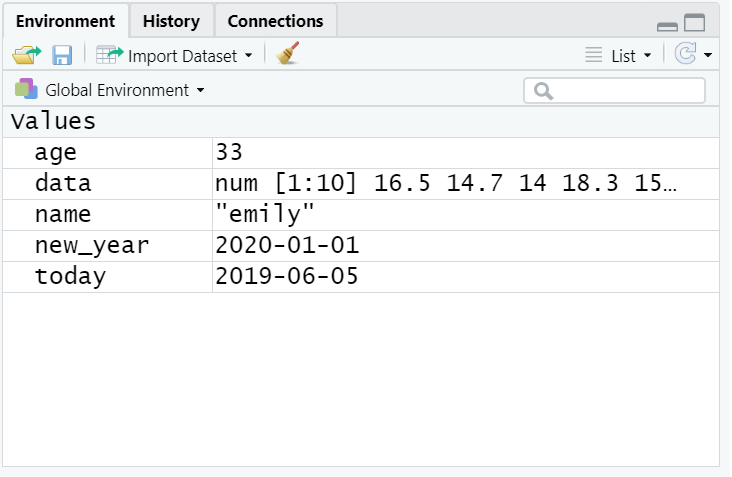
\includegraphics[width=1\linewidth]{images/objects-enviro} 

}

\caption{Objects in the environment}\label{fig:img-objects-enviro}
\end{figure}

Note that in these examples, \texttt{name},\texttt{age}, and \texttt{new\_year} would always contain the values \texttt{emily}, \texttt{35}, and the date of New Year's Day 2021, however, \texttt{today} will draw the date from the operating system and \texttt{data} will be a randomly generated set of data so the values of these objects will not be static.

As a side note, if you ever have to teach programming and statistics, don't use your age as an example because every time you have to update your teaching materials you get a reminder of the fragility of existence and your advancing age. 2021 update: I have now given up updating my age, I will remain forever 35.

Importantly, objects can be involved in calculations and can interact with each other. For example:

\begin{Shaded}
\begin{Highlighting}[]
\NormalTok{age }\SpecialCharTok{+} \DecValTok{10}
\NormalTok{new\_year }\SpecialCharTok{{-}}\NormalTok{ today}
\FunctionTok{mean}\NormalTok{(data)}
\end{Highlighting}
\end{Shaded}

\begin{verbatim}
## [1] 45
## Time difference of -260 days
## [1] 17.66644
\end{verbatim}

Finally, you can store the result of these operations in a new object:

\begin{Shaded}
\begin{Highlighting}[]
\NormalTok{decade }\OtherTok{\textless{}{-}}\NormalTok{ age }\SpecialCharTok{+} \DecValTok{10}
\end{Highlighting}
\end{Shaded}

\begin{try}
You may find it helpful to read \texttt{\textless{}-} as
\texttt{contains}, e.g., \texttt{name} contains the text \texttt{emily}.
\end{try}

You will constantly be creating objects throughout this course and you will learn more about them and how they behave as we go along, however, for now it is enough to understand that they are a way of saving values, that these values can be numbers, text, or the result of operations, and that they can be used in further operations to create new variables.

\begin{info}
You may also see objects referred to as `variables'. There is a
difference between the two in programming terms, however, they are used
synonymously very frequently.
\end{info}

\hypertarget{looking-after-the-environment}{%
\section{Looking after the environment}\label{looking-after-the-environment}}

If you've been writing a lot of code you may find that the environment pane (or workspace) has become cluttered with many objects. This can make it difficult to figure out which object you need and therefore you run the risk of using the wrong data frame. If you're working on a new dataset, or if you've tried lots of different code before getting the final version, it is good practice to remember to clear the environment to avoid using the wrong object. You can do this in several way.

\begin{enumerate}
\def\labelenumi{\arabic{enumi}.}
\tightlist
\item
  To remove individual objects, you can type \texttt{rm(object\_name)} in the console. Try this now to remove one of the objects you created in the previous section.
\item
  To clear all objects from the environment run \texttt{rm(list\ =\ ls())} in the console.
\item
  To clear all objects from the environment you can also click the broom icon in the environment pane.
\end{enumerate}

\begin{figure}

{\centering 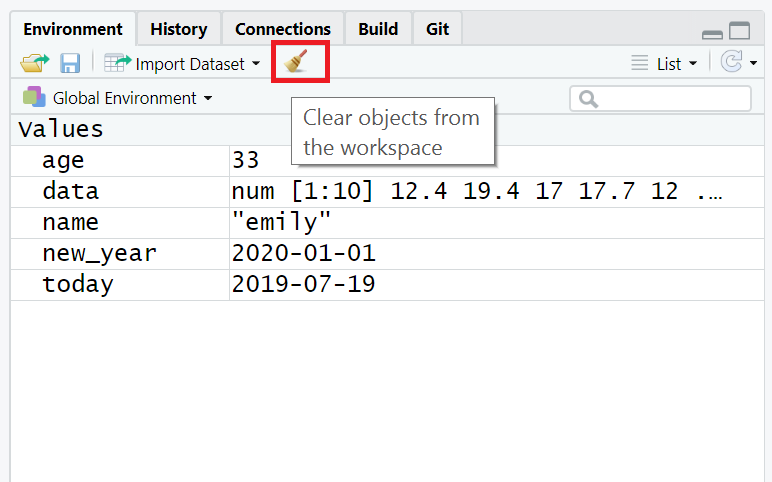
\includegraphics[width=1\linewidth]{images/broom} 

}

\caption{Clearing the workspace}\label{fig:img-broom}
\end{figure}

\hypertarget{global-options}{%
\section{Global options}\label{global-options}}

By default, when you open R Studio it will show you what you were last working on, including your code and any objects you have created. This might sound helpful, but actually it tends to cause more problems than it's worth because it means that you risk accidentally using an old version of an object. We recommend changing the settings so that each time you start R Studio, it opens a fresh copy. You can do this by clicking \texttt{Tools} - \texttt{Global\ Options} and then deselecting boxes so that it looks like the below.

\begin{figure}

{\centering 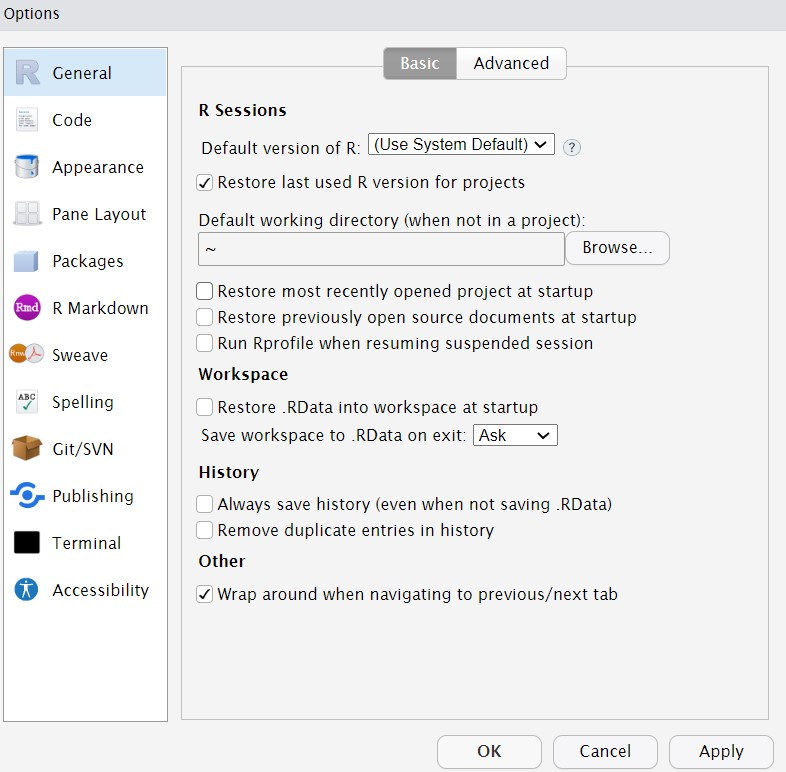
\includegraphics[width=1\linewidth]{images/global_options} 

}

\caption{Global options}\label{fig:img-options}
\end{figure}

\hypertarget{r-sessions}{%
\section{R sessions}\label{r-sessions}}

When you open up R and start writing code, loading packages, and creating objects, you're doing so in a new \textbf{session}. In addition to clearing the workspace, it can sometimes be useful to start a new session. This will happen automatically each time you start R on your computer, although sessions can persist on the server. If you find that your code isn't working and you can't figure out why, it might be worth starting a new session. This will clear the environment and detach all loaded packages - think of it like restarting your phone.

\hypertarget{activity-6}{%
\section{Activity 6}\label{activity-6}}

Click `Session - Restart R'.

\begin{figure}

{\centering 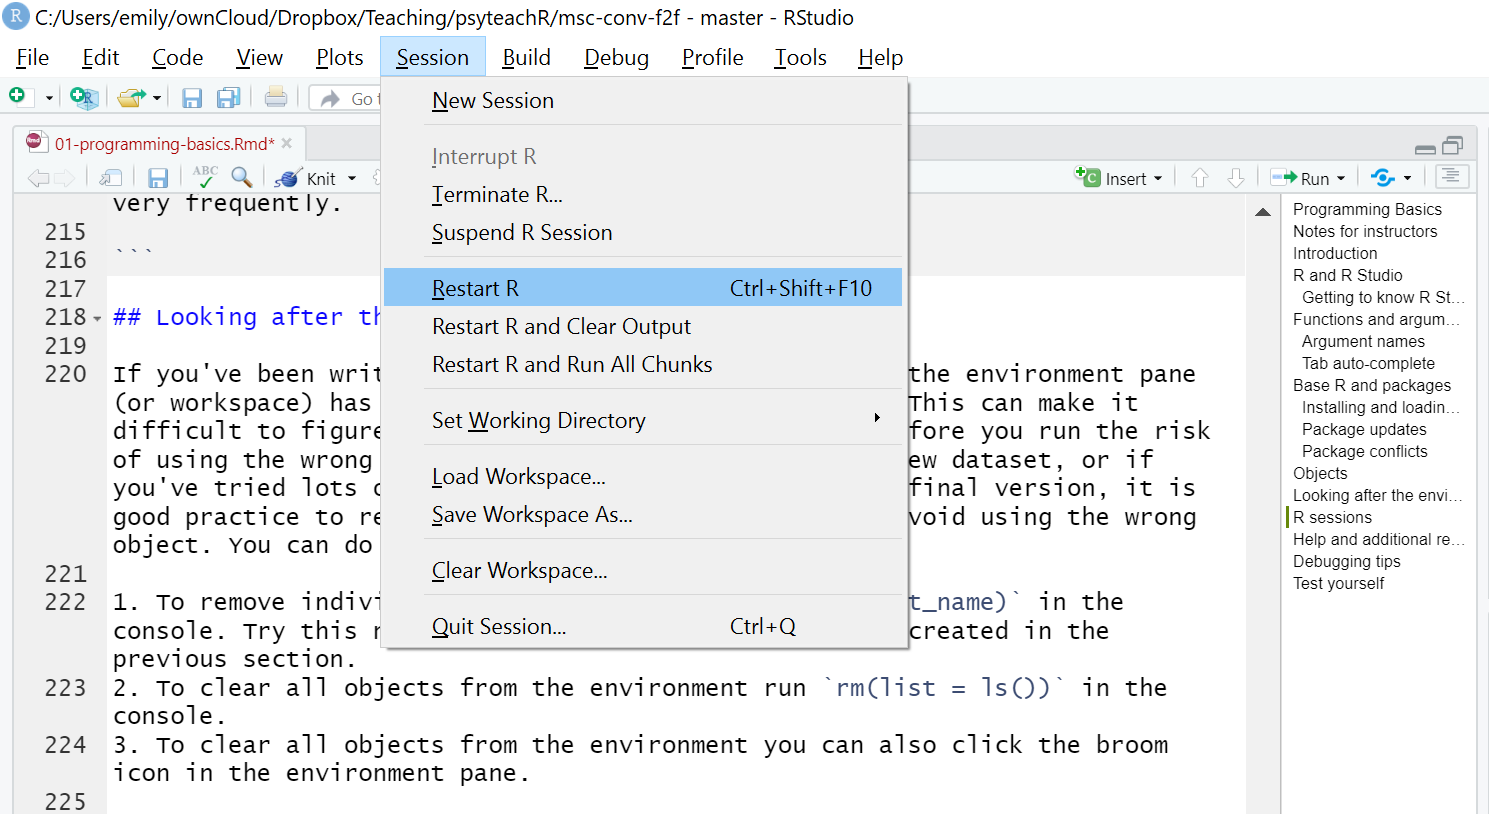
\includegraphics[width=1\linewidth]{images/new_session} 

}

\caption{The truth about programming}\label{fig:img-session}
\end{figure}

\hypertarget{how-to-cite-r-and-rstudio}{%
\section{How to cite R and RStudio}\label{how-to-cite-r-and-rstudio}}

You may be some way off writing a scientific report where you have to cite and reference R, however, when the time comes it is important to do so to the people who built it (most of them for free!) credit. You should provide separate citations for R, RStudio, and the packages you use.

To get the citation for the version of R you are using, simply run the \texttt{citation()} function which will always provide you with he most recent citation.

\begin{Shaded}
\begin{Highlighting}[]
\FunctionTok{citation}\NormalTok{()}
\end{Highlighting}
\end{Shaded}

\begin{verbatim}
## 
## To cite R in publications use:
## 
##   R Core Team (2021). R: A language and environment for statistical
##   computing. R Foundation for Statistical Computing, Vienna, Austria.
##   URL https://www.R-project.org/.
## 
## A BibTeX entry for LaTeX users is
## 
##   @Manual{,
##     title = {R: A Language and Environment for Statistical Computing},
##     author = {{R Core Team}},
##     organization = {R Foundation for Statistical Computing},
##     address = {Vienna, Austria},
##     year = {2021},
##     url = {https://www.R-project.org/},
##   }
## 
## We have invested a lot of time and effort in creating R, please cite it
## when using it for data analysis. See also 'citation("pkgname")' for
## citing R packages.
\end{verbatim}

To generate the citation for any packages you are using, you can also use the \texttt{citation()} function with the name of the package you wish to cite.

\begin{Shaded}
\begin{Highlighting}[]
\FunctionTok{citation}\NormalTok{(}\StringTok{"tidyverse"}\NormalTok{)}
\end{Highlighting}
\end{Shaded}

\begin{verbatim}
## 
##   Wickham et al., (2019). Welcome to the tidyverse. Journal of Open
##   Source Software, 4(43), 1686, https://doi.org/10.21105/joss.01686
## 
## A BibTeX entry for LaTeX users is
## 
##   @Article{,
##     title = {Welcome to the {tidyverse}},
##     author = {Hadley Wickham and Mara Averick and Jennifer Bryan and Winston Chang and Lucy D'Agostino McGowan and Romain François and Garrett Grolemund and Alex Hayes and Lionel Henry and Jim Hester and Max Kuhn and Thomas Lin Pedersen and Evan Miller and Stephan Milton Bache and Kirill Müller and Jeroen Ooms and David Robinson and Dana Paige Seidel and Vitalie Spinu and Kohske Takahashi and Davis Vaughan and Claus Wilke and Kara Woo and Hiroaki Yutani},
##     year = {2019},
##     journal = {Journal of Open Source Software},
##     volume = {4},
##     number = {43},
##     pages = {1686},
##     doi = {10.21105/joss.01686},
##   }
\end{verbatim}

To generate the citation for the version of RStudio you are using, you can use the \texttt{RStudio.Vesion()} function:

\begin{Shaded}
\begin{Highlighting}[]
\FunctionTok{RStudio.Version}\NormalTok{()}
\end{Highlighting}
\end{Shaded}

Finally, here's an example of how that might look in the write-up of your method section:

\begin{quote}
Analysis was conducted using R (R Core Team, 2020), RStudio (Rstudio Team, 2020), and the tidyverse package (Wickham, 2017).
\end{quote}

As noted, you may not have to do this for a while, but come back to this when you do as it's important to give the open-source community credit for their work.

\hypertarget{help-and-additional-resources}{%
\section{Help and additional resources}\label{help-and-additional-resources}}

Getting good at programming really means getting good trying stuff out, searching for help online, and finding examples of code to copy. If you are having difficulty with any of the exercises contained in this book then you can ask for help on Teams, however, learning to problem-solve effectively is a key skill that you need to develop throughout this course.

\begin{itemize}
\tightlist
\item
  Use the help documentation. If you're struggling to understand how a function works, remember the \texttt{?function} command.
\item
  If you get an error message, copy and paste it in to Google - it's very likely someone else has had the same problem.
\item
  In addition to these course materials there are a number of excellent resources for learning R:

  \begin{itemize}
  \tightlist
  \item
    \href{http://www.cookbook-r.com/}{R Cookbook}
  \item
    \href{https://stackoverflow.com/}{StackOverflow}
  \item
    \href{https://r4ds.had.co.nz/}{R for Data Science}
  \item
    Search or use the \href{https://twitter.com/search?f=tweets\&q=\%23rstats\&src=typd}{\#rstats} hashtag on Twitter
  \end{itemize}
\end{itemize}

\hypertarget{debugging-tips}{%
\section{Debugging tips}\label{debugging-tips}}

A large part of coding is trying to figure why your code doesn't work and this is true whether you are a novice or an expert. As you progress through this course you should keep a record of mistakes you make and how you fixed them. In each chapter we will provide a number of common mistakes to look out for but you will undoubtedly make (and fix!) new mistakes yourself.

\begin{itemize}
\tightlist
\item
  Have you loaded the correct packages for the functions you are trying to use? One very common mistake is to write the code to load the package, e.g., \texttt{library(tidyverse)} but then forget to run it.
\item
  Have you made a typo? Remember \texttt{data} is not the same as \texttt{DATA} and \texttt{t.test} is not the same as \texttt{t\_test}.
\item
  Is there a package conflict? Have you tried specifying the package and function with \texttt{package::function}?
\item
  Is it definitely an error? Not all red text in R means an error - sometimes it is just giving you a message with information.
\end{itemize}

\hypertarget{activity-6-test-yourself}{%
\section{Activity 6: Test yourself}\label{activity-6-test-yourself}}

\textbf{Question 1.} Why should you never include the code \texttt{install.packages()} in your analysis scripts? You should use library() insteadPackages are already part of Base RYou (or someone else) may accidentally install a package update that stops your code workingYou already have the latest version of the package

Explain This Answer

Remember, when you run \texttt{install.packages()} it will always install the latest version of the package and it will overwrite any older versions of the package you may have installed.

\textbf{Question 2.}What will the following code produce?

\begin{Shaded}
\begin{Highlighting}[]
\FunctionTok{rnorm}\NormalTok{(}\DecValTok{6}\NormalTok{, }\DecValTok{50}\NormalTok{, }\DecValTok{10}\NormalTok{)}
\end{Highlighting}
\end{Shaded}

A dataset with 10 numbers that has a mean of 6 and an SD of 50A dataset with 6 numbers that has a mean of 50 and an SD of 10A dataset with 50 numbers that has a mean of 10 and an SD of 6A dataset with 50 numbers that has a mean of 10 and an SD of 6

Explain This Answer

The default form for \texttt{rnorm()} is \texttt{rnorm(n,\ mean,\ sd)}. If you need help remembering what each argument of a function does, look up the help documentation by running \texttt{?rnorm}

\textbf{Question 3.} If you have two packages that have functions with the same name and you want to specify exactly which package to use, what code would you use?

package::functionfunction::packagelibrary(package)install.packages(package)

Explain This Answer

You should use the form \texttt{package::function}, for example \texttt{dplyr::select}. Remember that when you first load your packages R will warn you if any functions have the same name - remember to look out for this!

\textbf{Question 4.} Which of the following is most likely to be an argument? 35read\_csv()\textless-

\textbf{Question 5.} An easy way to spot functions is to look for bracketsnumberscomputers.

\textbf{Question 6.} The job of \texttt{\textless{}-} is to send the output from the function to a/an argumentassignmentobject.

\hypertarget{ref1}{%
\chapter{Intro to R}\label{ref1}}

There are eight activities in total for this chapter, but don't worry, they are broken down into very small steps!

\hypertarget{walkthrough-video}{%
\section{Walkthrough video}\label{walkthrough-video}}

There is a \href{https://uofglasgow.zoom.us/rec/play/uJ_2RvnP_UhUF7jM7hQZzOD6KjqjUm1UmPupTfFHBAftxrpMScYWRxkeuzGG0g0RqeE2UBCSmAO5riBo.6AKR_E01noBaq4-b?autoplay=true\&startTime=1600178959000}{walkthrough video} of this chapter available via Zoom.

\begin{itemize}
\tightlist
\item
  Video notes: this video was recorded in September 2020 when we recommended using the server above installing R on your computer. With more experience of the server, we now strongly encourage you to install R on your computer if you can. The book has also been updated visually but there are no other differences between the video and this book chapter in terms of content.
\end{itemize}

\hypertarget{activity-1-upload-data-files-to-the-server}{%
\section{Activity 1: Upload data files to the server}\label{activity-1-upload-data-files-to-the-server}}

The main disadvantage to using the R server is that you need to upload and download any files you are working on to and from the server (if you are using a local installation on your laptop you can skip this step).

In \href{https://psyteachr.github.io/ug1-practical/getting-to-know-the-data.html\#activity-2}{Getting to know the data} you downloaded the data files we will be using for this semester. In order to use these files, we need to copy them to the R server. Whilst we're not going to use the data in this chapter, it's a useful step to get ready for next week.

\begin{itemize}
\tightlist
\item
  Log on to the \href{https://rstudio.psy.gla.ac.uk/}{R server}
\item
  In the Files pane, click \texttt{New\ folder} and call it Psych 1A.
\item
  Click \texttt{Upload} then \texttt{Browse}and choose the Psych 1A folder that you just created.
\item
  Click \texttt{Choose\ file} and go and find the \textbf{zip folder} that you downloaded in \href{https://psyteachr.github.io/ug1-practical/getting-to-know-the-data.html\#activity-2}{Getting to know the data} (if you deleted it you can download it again). Using the zip folder means you can upload multiple files at once rather than one at a time.
\item
  Once you have uploaded the zip file, the server will automatically unzip the files and you should be able to see all the files you have on your computer.
\end{itemize}

Please be aware that \textbf{there is no link between your computer and the R server}. If you change files on the server, they won't magically appear on your computer and you need to be very careful when you submit your homework files that you're submitting the right thing (last year we had lots of student submit blank files). This is the main reason we recommend installing R on your computer if you can.

\hypertarget{activity-2-set-the-working-directory}{%
\section{Activity 2: Set the working directory}\label{activity-2-set-the-working-directory}}

Once you have uploaded the data, set the working directory by clicking \texttt{Session} -\textgreater{} \texttt{Set\ Working\ Directory} -\textgreater{} \texttt{Choose\ Directory} and then select the Data Skills 1A folder as your working directory.

You need to do this step regardless of whether you are working from the server or from your laptop. This means that R knows which folder to look in for the data and scripts you might want to use.
\#\# R Markdown for data skills work and homework assignments

For the data skills work and homework you will use a worksheet format called R Markdown (abbreviated as Rmd) which is a great way to create dynamic documents with embedded chunks of code. These documents are self-contained and fully reproducible (if you have the necessary data, you should be able to run someone else's analyses with the click of a button) which makes it very easy to share. This is an important part of your open science training as one of the reasons we are using R and RStudio is that it enables us to share open and reproducible information. Using these worksheets enables you to keep a record of all the code you write, and when it comes time for the portfolio assignments, we can give you a task and you can fill in the required code.

For more information about R Markdown feel free to have a look at their main webpage \url{http://rmarkdown.rstudio.com}. The key advantage of R Markdown is that it allows you to write code into a document, along with regular text, and then \textbf{knit} it using the package \texttt{knitr} to create your document as either a webpage (HTML), a PDF, or Word document (.docx).

\hypertarget{activity-3-open-and-save-a-new-r-markdown-document}{%
\section{Activity 3: Open and save a new R Markdown document}\label{activity-3-open-and-save-a-new-r-markdown-document}}

To open a new R Markdown document click the `new item' icon and then click `R Markdown'. You will be prompted to give it a title, call it ``Intro to R''. Also, change the author name to your GUID as this will be good practice for the homework. Keep the output format as HTML.

Once you've opened a new document be sure to save it by clicking \texttt{File} -\textgreater{} \texttt{Save\ as}. You should also name this file ``Intro to R''. If you've set the working directory correctly, you should now see this file appear in your file viewer pane.

\begin{figure}

{\centering 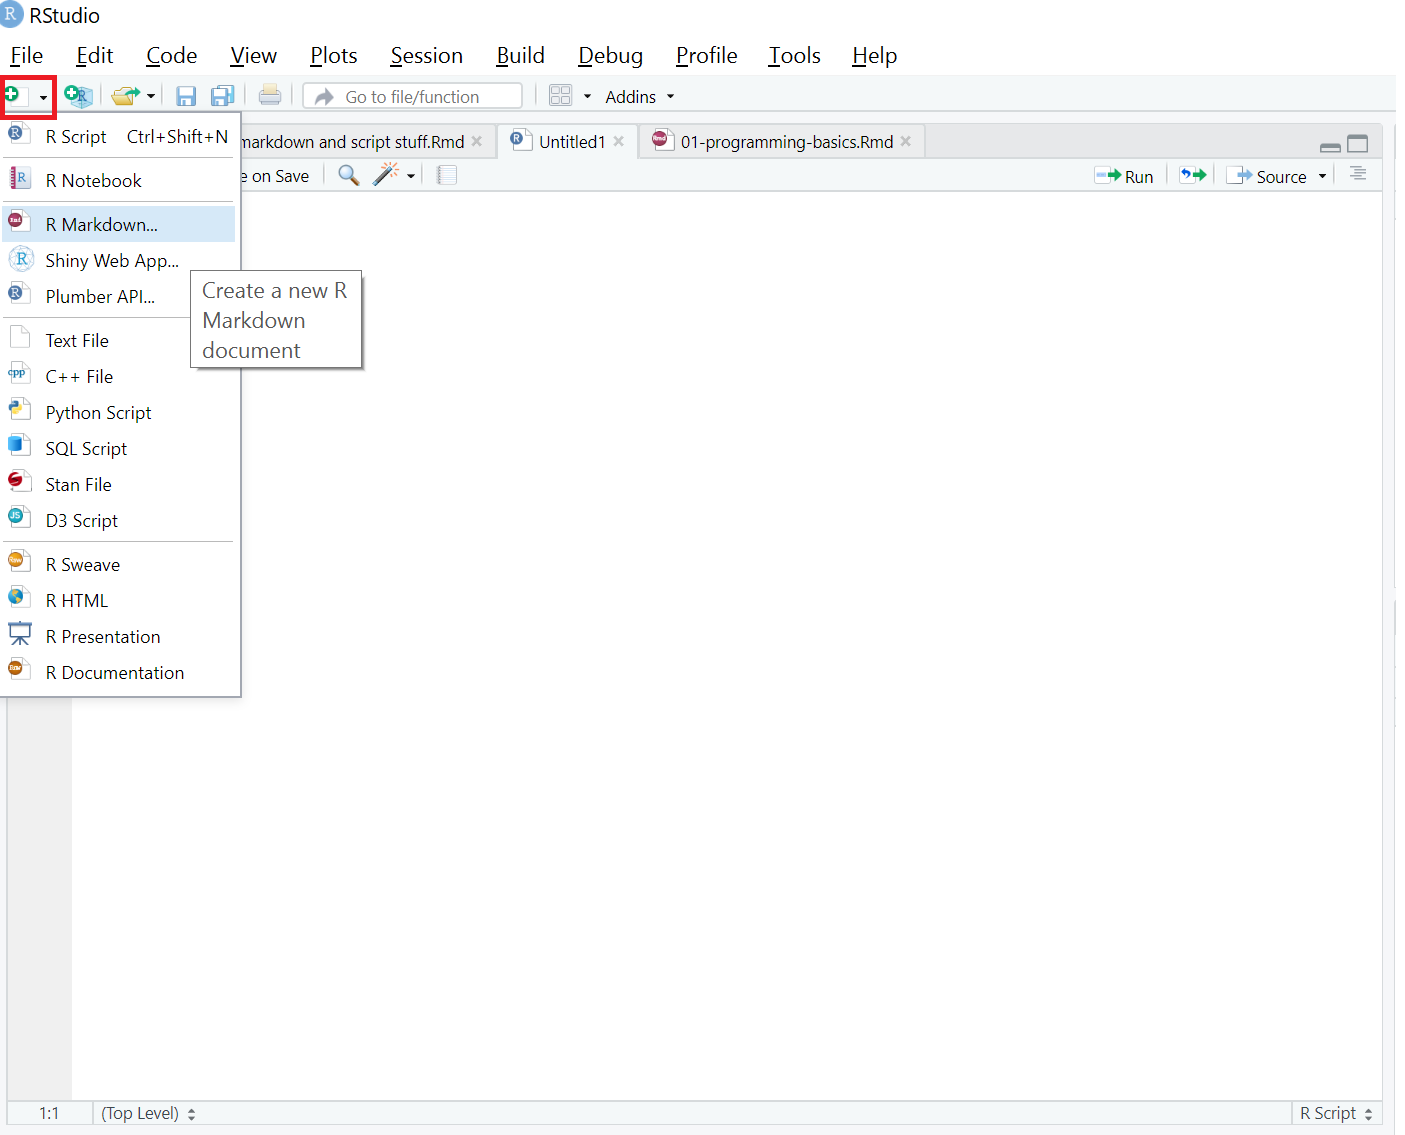
\includegraphics[width=1\linewidth]{images/new-markdown} 

}

\caption{Opening a new R Markdown document}\label{fig:img-new-markdown}
\end{figure}

\hypertarget{activity-4-create-a-new-code-chunk}{%
\section{Activity 4: Create a new code chunk}\label{activity-4-create-a-new-code-chunk}}

When you first open a new R Markdown document you will see a bunch of welcome text that looks like this:

\begin{figure}

{\centering 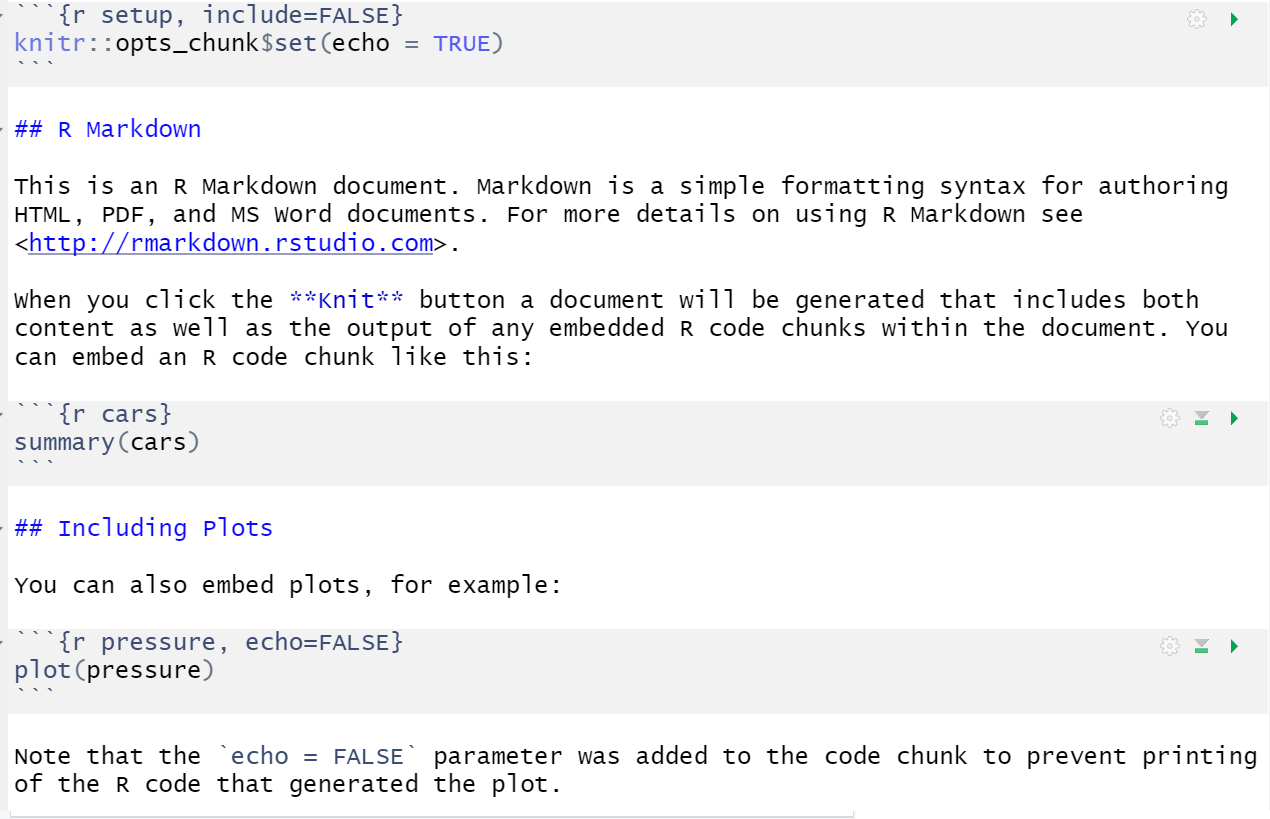
\includegraphics[width=1\linewidth]{images/markdown-default} 

}

\caption{New R Markdown text}\label{fig:img-markdown-default}
\end{figure}

Do the following steps:\\
* Delete \textbf{everything} below line 7\\
* On line 8 type ``About me''\\
* Click \texttt{Insert} -\textgreater{} \texttt{R}

Your Markdown document should now look something like this:

\begin{figure}

{\centering 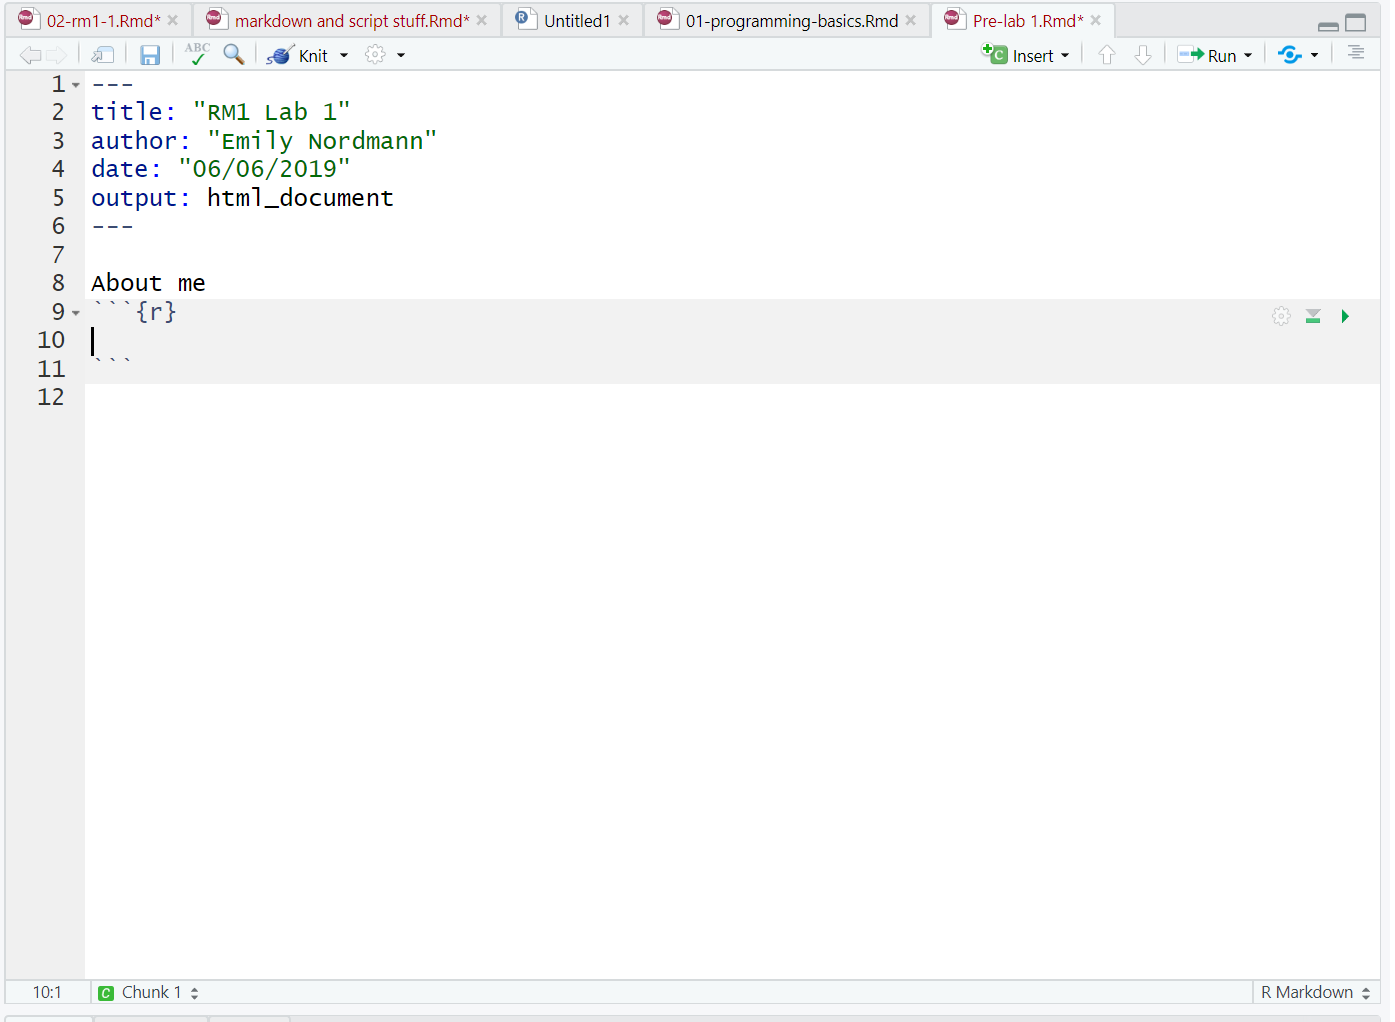
\includegraphics[width=1\linewidth]{images/new-chunk} 

}

\caption{New R chunk}\label{fig:img-new-chunk}
\end{figure}

What you have created is a \textbf{code chunk}. In R Markdown, anything written in the white space is regarded as normal text, and anything written in a grey code chunk is assumed to be code. This makes it easy to combine both text and code in one document.

\begin{warning}
When you create a new code chunk you should notice that the grey box
starts and ends with three back ticks ```. One common mistake is to
accidentally delete these back ticks. Remember, code chunks are grey and
text entry is white - if the colour of certain parts of your Markdown
doesn't look right, check that you haven't deleted the back ticks.
\end{warning}

\hypertarget{activity-5-write-some-code}{%
\section{Activity 5: Write some code}\label{activity-5-write-some-code}}

Now we're going to use the code examples you read about in Programming Basics to add some simple code to our R Markdown document.

\begin{itemize}
\tightlist
\item
  In your code chunk write the below code but replace the values of name/age/birthday with your own details).\\
\item
  Note that text values and dates need to be contained in quotation marks but numerical values do not. Missing and/or unnecessary quotation marks are a common cause of code not working - remember this!
\end{itemize}

\begin{Shaded}
\begin{Highlighting}[]
\NormalTok{name }\OtherTok{\textless{}{-}} \StringTok{"Emily"} 
\NormalTok{age }\OtherTok{\textless{}{-}} \DecValTok{35}
\NormalTok{today }\OtherTok{\textless{}{-}} \FunctionTok{Sys.Date}\NormalTok{()}
\NormalTok{next\_birthday }\OtherTok{\textless{}{-}} \FunctionTok{as.Date}\NormalTok{(}\StringTok{"2021{-}07{-}11"}\NormalTok{)}
\end{Highlighting}
\end{Shaded}

\hypertarget{running-code}{%
\section{Running code}\label{running-code}}

When you're working in an R Markdown document, there are several ways to run your lines of code.

First, you can highlight the code you want to run and then click \texttt{Run} -\textgreater{} \texttt{Run\ Selected\ Line(s)}, however this is very slow.

\begin{figure}

{\centering \includegraphics[width=1\linewidth]{images/run1} 

}

\caption{Slow method of running code}\label{fig:img-run1}
\end{figure}

Alternatively, you can press the green ``play'' button at the top-right of the code chunk and this will run \textbf{all} lines of code in that chunk.

\begin{figure}

{\centering \includegraphics[width=1\linewidth]{images/run2} 

}

\caption{Slightly better method of running code}\label{fig:img-run2}
\end{figure}

Even better though is to learn some of the keyboard shortcuts for R Studio. To run a single line of code, make sure that the cursor is in the line of code you want to run (it can be anywhere) and press \texttt{ctrl\ +\ enter}. If you want to run all of the code in the code chunk, press \texttt{ctrl\ +\ shift\ +\ enter}. Learn these shortcuts, they will make your life easier!

\hypertarget{activity-6-run-your-code}{%
\section{Activity 6: Run your code}\label{activity-6-run-your-code}}

Run your code using one of the methods above. You should see the variables \texttt{name}, \texttt{age}, \texttt{today}, and \texttt{next\_birthday} appear in the environment pane.

\hypertarget{activity-7-inline-code}{%
\section{Activity 7: Inline code}\label{activity-7-inline-code}}

An incredibly useful feature of R Markdown is that R can insert values into your writing using \textbf{inline code}. If you've ever had to copy and paste a value or text from one file in to another, you'll know how easy it can be to make mistakes. Inline code avoids this. It's easier to show you what inline code does rather than to explain it so let's have a go.

First, copy and paste this text exactly (do not change anything) to the \textbf{white space} underneath your code chunk.

\begin{Shaded}
\begin{Highlighting}[]
\NormalTok{My name is }\StringTok{\textasciigrave{}}\AttributeTok{r name}\StringTok{\textasciigrave{}}\NormalTok{ and I am }\StringTok{\textasciigrave{}}\AttributeTok{r age}\StringTok{\textasciigrave{}}\NormalTok{ years old. It is }\StringTok{\textasciigrave{}}\AttributeTok{r next\_birthday {-} today}\StringTok{\textasciigrave{}}\NormalTok{ days until my birthday.}
\end{Highlighting}
\end{Shaded}

\hypertarget{activity-8-knitting-your-file}{%
\section{Activity 8: Knitting your file}\label{activity-8-knitting-your-file}}

Nearly finished! As our final step we are going to ``knit'' our file. This simply means that we're going to compile our code into a document that is more presentable. To do this click \texttt{Knit} -\textgreater{} \texttt{Knit\ to\ HMTL}. R Markdown will create a new HTML document and it will automatically save this file in your working directory.

As if by magic, that slightly odd bit of text you copied and pasted now appears as a normal sentence with the values pulled in from the objects you created.

\textbf{My name is Emily and I am 35 years old. It is -69 days until my birthday.}

We're not going to use this function very often in the rest of the course but hopefully you can see just how useful this would be when writing up a report with lots of numbers! R Markdown is an incredibly powerful and flexible format - this book was written using it! If you want to push yourself with R, additional functions and features of R Markdown would be a good place to start.

Before we finish, there are a few final things to note about knitting that will be useful for the homework:

\begin{itemize}
\tightlist
\item
  R Markdown will only knit if your code works - this is a good way of checking for the homework assignments whether you've written legal code!\\
\item
  You can choose to knit to a Word document rather than HTML. This can be useful for e.g., sharing with others, however, it may lose some functionality and it probably won't look as good so we'd recommend always knitting to HTML.
\item
  You can choose to knit to PDF, however, unless you're using the server this requires an LaTex installation and is quite complicated. If you don't already know what LaTex is and how to use it, do not knit to PDF. If you do know how to use LaTex, you don't need us to give you instructions!
\item
  R will automatically open the knitted HTML file in the viewer, however, you can also navigate to the folder it is stored in and open the HTML file in your web browser (e.g., Chrome or Firefox).
\end{itemize}

\hypertarget{activity-9-make-r-your-own}{%
\section{Activity 9: Make R your own}\label{activity-9-make-r-your-own}}

Finally, you can customise how R Studio looks to make it feel more like your own personal version. Click \texttt{Tools} - \texttt{Global\ Options} - \texttt{Appearance}. You can change the default font, font size, and general appearance of R Studio, including using dark mode. Play around with the settings and see which one you prefer - you're going to spend a lot of time with R, it might as well look nice!

\hypertarget{finished}{%
\section{Finished}\label{finished}}

And you're done! On your very first time using R you've not only written functioning code but you've written a reproducible output! You could send someone else your R Markdown document and they would be able to produce exactly the same HTML document as you, just by pressing knit.

The key thing we want you to take away from this chapter is that R isn't scary. It might be very new to a lot of you, but we're going to take you through it step-by-step. You'll be amazed at how quickly you can start producing professional-looking data visualisations and analysis.

If you're using the server, we recommend that you download any files that you have been working on so that you have a backup.

\hypertarget{loading-data}{%
\chapter{Loading data}\label{loading-data}}

Part of becoming a psychologist is asking questions and gathering data to enable you to answer these questions effectively. It is very important that you understand all aspects of the research process such as experimental design, ethics, data management and visualisation.

In this chapter, you will continue to develop reproducible scripts. This means scripts that completely and transparently perform an analysis from start to finish in a way that yields the same result for different people using the same software on different computers. And transparency is a key value of science, as embodied in the ``trust but verify'' motto. When you do things reproducibly, others can understand and check your work.

This benefits science, but there is a selfish reason, too: the most important person who will benefit from a reproducible script is your future self. When you return to an analysis after two weeks of vacation, you will thank your earlier self for doing things in a transparent, reproducible way, as you can easily pick up right where you left off.

As part of your skill development, it is important that you work with data so that you can become confident and competent in your management and analysis of data. In all of your psychology data skills courses, we will work with real data that has been shared by other researchers.

\hypertarget{getting-data-ready-to-work-with}{%
\section{Getting data ready to work with}\label{getting-data-ready-to-work-with}}

In this chapter you will learn how to load the packages required to work with our data. You'll then load the data into R Studio before getting it organised into a sensible format that relates to our research question. If you can't remember what packages are, go back and revise \ref{packages}.

\hypertarget{walkthrough-video-1}{%
\section{Walkthrough video}\label{walkthrough-video-1}}

There is a \href{https://uofglasgow.zoom.us/rec/play/teIkYYMpGx6UZyRmnp6oFP9a0oR1pkAdyKDtrOS19PMrPzWFD6UM8kf1JPOA8BUCvdTjDD1TL0BY7fst.UJ5avFdQMYGeSE-b?startTime=1600350969000\&_x_zm_rtaid=tV6tnLfOQS6SzFo0htAAPg.1600855466001.bb934ef09570772957442af0f1cfb9b5\&_x_zm_rhtaid=682}{walkthrough video} of this chapter available via Zoom.

\begin{itemize}
\tightlist
\item
  Video notes: this video was recorded in 2020 when we recommended using the server above installing R on your computer. With more experience of the server, we now strongly encourage you to install R on your computer if you can. There are no other differences between the video and this book chapter.
\end{itemize}

\hypertarget{stub-files}{%
\section{Stub files}\label{stub-files}}

When you downloaded the data in Getting to know the data, you will have noticed that there were five Rmd files that all started with \texttt{stub-}. These stub files are set-up with code chunks for each activity of the chapter to help make your life a bit easier as you are first learning to code. We will take these away in Psych 1B but for this semester, you don't need to set up your own file, just open the relevant stub file for each chapter.

\hypertarget{activity-1-set-up}{%
\section{Activity 1: Set-up}\label{activity-1-set-up}}

Before we begin working with the data we need to do some set-up. If you need help with any of these steps, you should refer to Chapter \ref{ref1}:

\begin{itemize}
\tightlist
\item
  You should have already downloaded the data files and, if you are using the server, uploaded them to the R server as part of \href{https://psyteachr.github.io/ug1-practical/ref1.html}{Intro to R}, if you haven't done this, go back and work through that chapter now.
\item
  Open R and ensure the environment is clear.
\item
  If you're on the server, avoid a number of issues by restarting the session - click \texttt{Session} - \texttt{Restart\ R}\\
\item
  Set the working directory to your Data Skills folder.\\
\item
  Open the \texttt{stub-loading-data} file and ensure that the working directory is set to your Data Skills folder and that the two .csv data files are in your working directory (you should see them in the file pane).
\end{itemize}

\hypertarget{activity-2-load-in-the-package}{%
\section{Activity 2: Load in the package}\label{activity-2-load-in-the-package}}

Today we need to use the \texttt{tidyverse} package. You will use this package in almost every single chapter on this course as the functions it contains are those we use for data wrangling, descriptive statistics, and visualisation.

\begin{itemize}
\tightlist
\item
  To load the \texttt{tidyverse} type the following code into your \textbf{code chunk} (not the console) and then run it.
\end{itemize}

\begin{Shaded}
\begin{Highlighting}[]
\FunctionTok{library}\NormalTok{(tidyverse)}
\end{Highlighting}
\end{Shaded}

\hypertarget{open-data}{%
\section{Open data}\label{open-data}}

For this chapter we are going to be using the real dataset that you looked at in Getting to Know the Data. Click the below link if you want a refresher of what the dataset contains.

\href{https://openpsychologydata.metajnl.com/articles/10.5334/jopd.35/}{Woodworth, R.J., O'Brien-Malone, A., Diamond, M.R. and Schüz, B., 2018. Data from, `Web-based Positive Psychology Interventions: A Reexamination of Effectiveness'. Journal of Open Psychology Data, 6(1).}

\hypertarget{activity-3-read-in-data}{%
\section{Activity 3: Read in data}\label{activity-3-read-in-data}}

Now we can read in the data. To do this we will use the function \texttt{read\_csv()} that allows us to read in .csv files. There are also functions that allow you to read in .xlsx files and other formats, however in this course we will only use .csv files.

\begin{itemize}
\tightlist
\item
  First, we will create an object called \texttt{dat} that contains the data in the \texttt{ahi-cesd.csv} file. Then, we will create an object called \texttt{info} that contains the data in the \texttt{participant-info.csv}.
\end{itemize}

\begin{Shaded}
\begin{Highlighting}[]
\NormalTok{dat }\OtherTok{\textless{}{-}} \FunctionTok{read\_csv}\NormalTok{ (}\StringTok{"ahi{-}cesd.csv"}\NormalTok{)}
\NormalTok{pinfo }\OtherTok{\textless{}{-}} \FunctionTok{read\_csv}\NormalTok{(}\StringTok{"participant{-}info.csv"}\NormalTok{)}
\end{Highlighting}
\end{Shaded}

\begin{danger}
There is also a function called \texttt{read.csv()}. Be very careful NOT
to use this function instead of \texttt{read\_csv()} as they have
different ways of naming columns. For the homework, unless your results
match ours \textbf{exactly} you will not get the marks which means you
need to be careful to use the right functions.
\end{danger}

\hypertarget{activity-4-check-your-data}{%
\section{Activity 4: Check your data}\label{activity-4-check-your-data}}

You should now see that the objects \texttt{dat} and \texttt{pinfo} have appeared in the environment pane. Whenever you read data into R you should always do an initial check to see that your data looks like you expected. There are several ways you can do this, try them all out to see how the results differ.

\begin{itemize}
\tightlist
\item
  In the environment pane, click on \texttt{dat} and \texttt{pinfo}. This will open the data to give you a spreadsheet-like view (although you can't edit it like in Excel)
\item
  In the environment pane, click the small blue play button to the left of \texttt{dat} and \texttt{pinfo}. This will show you the structure of the object information including the names of all the variables in that object and what type they are (also see \texttt{str(pinfo)})
\item
  Use \texttt{summary(pinfo)}
\item
  Use \texttt{head(pinfo)}
\item
  Just type the name of the object you want to view, e.g., \texttt{dat}.
\end{itemize}

\hypertarget{activity-5-join-the-files-together}{%
\section{Activity 5: Join the files together}\label{activity-5-join-the-files-together}}

We have two files, \texttt{dat} and \texttt{info} but what we really want is a single file that has both the data and the demographic information about the participants. R makes this very easy by using the function \texttt{inner\_join()}.

Remember to use the help function \texttt{?inner\_join} if you want more information about how to use a function and to use tab auto-complete to help you write your code.

The below code will create a new object \texttt{all\_dat} that has the data from both \texttt{dat} and \texttt{pinfo} and it will use the columns \texttt{id} and \texttt{intervention} to match the participants' data. If you want to join tables that have multiple columns in common, you need to use \texttt{c()} to list them all (I think of it as c for combine, or collection).

\begin{itemize}
\tightlist
\item
  Run this code and then view the new dataset using one of the methods from Activity 4.
\end{itemize}

\begin{Shaded}
\begin{Highlighting}[]
\NormalTok{all\_dat }\OtherTok{\textless{}{-}} \FunctionTok{inner\_join}\NormalTok{(}\AttributeTok{x =}\NormalTok{ dat, }\CommentTok{\# the first table you want to join}
                      \AttributeTok{y =}\NormalTok{ pinfo, }\CommentTok{\# the second table you want to join}
                      \AttributeTok{by =} \FunctionTok{c}\NormalTok{(}\StringTok{"id"}\NormalTok{, }\StringTok{"intervention"}\NormalTok{)) }\CommentTok{\# columns the two tables have in common}
\end{Highlighting}
\end{Shaded}

\hypertarget{activity-6-pull-out-variables-of-interest}{%
\section{Activity 6: Pull out variables of interest}\label{activity-6-pull-out-variables-of-interest}}

Our final step is to pull our variables of interest. Very frequently, datasets will have more variables and data than you actually want to use and it can make life easier to create a new object with just the data you need.

In this case, the file contains the responses to each individual question on both the AHI scale and the CESD scale as well as the total score (i.e., the sum of all the individual responses). For our analysis, all we care about is the total scores, as well as the demographic information about participants.

To do this we use the \texttt{select()} function to create a new object named \texttt{summarydata}.

\begin{Shaded}
\begin{Highlighting}[]
\NormalTok{summarydata }\OtherTok{\textless{}{-}} \FunctionTok{select}\NormalTok{(}\AttributeTok{.data =}\NormalTok{ all\_dat, }\CommentTok{\# name of the object to take data from}
\NormalTok{                      ahiTotal, cesdTotal, sex, age, educ, income, occasion,elapsed.days) }\CommentTok{\# all the columns you want to keep}
\end{Highlighting}
\end{Shaded}

\begin{danger}
If you get an error message when using select that says
\texttt{unused\ argument} it means that it is trying to use the wrong
version of the select function. There are two solutions to this, first,
save you work and then restart the R session (click session -restart R)
and then run all your code above again from the start, or replace
\texttt{select} with \texttt{dplyr::select} which tells R exactly which
version of the select function to use. We'd recommend restarting the
session because this will get you in the habit and it's a useful thing
to try for a range of problems
\end{danger}

\begin{itemize}
\tightlist
\item
  Run the above code and then run \texttt{head(summarydata)}. If everything has gone to plan it should look something like this:
\end{itemize}

\hypertarget{activity-7-visualise-the-data}{%
\section{Activity 7: Visualise the data}\label{activity-7-visualise-the-data}}

As you're going to learn about more over this course, data visualisation is extremely important. Visualisations can be used to give you more information about your dataset, but they can also be used to mislead.

We're going to look at how to write the code to produce simple visualisations in a few weeks, for now, we want to focus on how to read and interpret different kinds of graphs. Please feel free to play around with the code and change \texttt{TRUE} to \texttt{FALSE} and adjust the values and labels and see what happens but do not worry about understanding the code. Just copy and paste it.

Copy, paste and run the below code to produce a bar graph that shows the number of female and male participants in the dataset.

\begin{Shaded}
\begin{Highlighting}[]
\FunctionTok{ggplot}\NormalTok{(summarydata, }\FunctionTok{aes}\NormalTok{(}\AttributeTok{x =} \FunctionTok{as.factor}\NormalTok{(sex), }\AttributeTok{fill =} \FunctionTok{as.factor}\NormalTok{(sex))) }\SpecialCharTok{+}
  \FunctionTok{geom\_bar}\NormalTok{(}\AttributeTok{show.legend =} \ConstantTok{FALSE}\NormalTok{, }\AttributeTok{alpha =}\NormalTok{ .}\DecValTok{8}\NormalTok{) }\SpecialCharTok{+}
  \FunctionTok{scale\_x\_discrete}\NormalTok{(}\AttributeTok{name =} \StringTok{"Sex"}\NormalTok{) }\SpecialCharTok{+}
  \FunctionTok{scale\_fill\_viridis\_d}\NormalTok{(}\AttributeTok{option =} \StringTok{"E"}\NormalTok{) }\SpecialCharTok{+}
  \FunctionTok{scale\_y\_continuous}\NormalTok{(}\AttributeTok{name =} \StringTok{"Number of participants"}\NormalTok{)}\SpecialCharTok{+}
  \FunctionTok{theme\_minimal}\NormalTok{()}
\end{Highlighting}
\end{Shaded}

Are there more male or more female participants (you will need to check the codebook to find out what 1 and 2 mean to answer this)? More female participantsMore male participants

Copy, paste, and run the below code to create violin-boxplots of happiness scores for each income group.

\begin{Shaded}
\begin{Highlighting}[]
\FunctionTok{ggplot}\NormalTok{(summarydata, }\FunctionTok{aes}\NormalTok{(}\AttributeTok{x =} \FunctionTok{as.factor}\NormalTok{(income), }\AttributeTok{y =}\NormalTok{ ahiTotal, }\AttributeTok{fill =} \FunctionTok{as.factor}\NormalTok{(income))) }\SpecialCharTok{+}
  \FunctionTok{geom\_violin}\NormalTok{(}\AttributeTok{trim =} \ConstantTok{FALSE}\NormalTok{, }\AttributeTok{show.legend =} \ConstantTok{FALSE}\NormalTok{, }\AttributeTok{alpha =}\NormalTok{ .}\DecValTok{4}\NormalTok{) }\SpecialCharTok{+}
  \FunctionTok{geom\_boxplot}\NormalTok{(}\AttributeTok{width =}\NormalTok{ .}\DecValTok{2}\NormalTok{, }\AttributeTok{show.legend =} \ConstantTok{FALSE}\NormalTok{, }\AttributeTok{alpha =}\NormalTok{ .}\DecValTok{7}\NormalTok{)}\SpecialCharTok{+}
  \FunctionTok{scale\_x\_discrete}\NormalTok{(}\AttributeTok{name =} \StringTok{"Income"}\NormalTok{, }\AttributeTok{labels =} \FunctionTok{c}\NormalTok{(}\StringTok{"Below Average"}\NormalTok{, }\StringTok{"Average"}\NormalTok{, }\StringTok{"Above Average"}\NormalTok{)) }\SpecialCharTok{+}
  \FunctionTok{scale\_y\_continuous}\NormalTok{(}\AttributeTok{name =} \StringTok{"Authentic Happiness Inventory Score"}\NormalTok{)}\SpecialCharTok{+}
  \FunctionTok{theme\_minimal}\NormalTok{() }\SpecialCharTok{+}
  \FunctionTok{scale\_fill\_viridis\_d}\NormalTok{()}
\end{Highlighting}
\end{Shaded}

\begin{itemize}
\tightlist
\item
  The violin (the wavy line) shows density. Basically, the fatter the wavy shape, the more data points there are at that point. It's called a violin plot because it very often looks (kinda) like a violin.
\item
  The boxplot is the box in the middle. The black line shows the median score in each group. The median is calculated by arranging the scores in order from the smallest to the largest and then selecting the middle score.
\item
  The other lines on the boxplot show the interquartile range. There is a really good explanation of \href{https://medium.com/dayem-siddiqui/understanding-and-interpreting-box-plots-d07aab9d1b6c}{how to read a boxplot here}.
\item
  The black dots are outliers, i.e., extreme values.
\end{itemize}

Which income group has the highest median happiness score? Below averageAverageAbove average

Which income group has the lowest median happiness score? Below averageAverage

How many outliers does the Average income group have?

Finally, try knitting the file to HTML. And that's it, well done! Remember to save your Markdown in your Data Skills folder and make a note of any mistakes you made and how you fixed them.

\hypertarget{finished-1}{%
\subsection{Finished!}\label{finished-1}}

Well done! You have started on your journey to become a confident and competent member of the open science community! To show us how competent you are you should now complete the homework for this week which follows the same instructions as this in-class activity but asks you to work with different variables. Always use the data skills materials and videos to help you complete the assessments!

Finally, if you're working from the R server, we'd recommend that you download a copy of the changes you've made to \texttt{stub-loading-data} so that you have a backup.

\hypertarget{debugging-tips-1}{%
\section{Debugging tips}\label{debugging-tips-1}}

\begin{itemize}
\tightlist
\item
  When you downloaded and uploaded the files did you save the file names \textbf{exactly} as they were originally? If you download the file more than once you will find your computer may automatically add a number to the end of the file name. \texttt{data.csv} is not the same as \texttt{data(1).csv}. Pay close attention to names!
\item
  Have you used the \textbf{exact} same object names as we did in each activity? Remember, \texttt{name} is different to \texttt{Name}. In order to make sure you can follow along with this book, pay special attention to ensuring you use the same object names as we do.\\
\item
  Have you used quotation marks where needed?\\
\item
  Have you accidentally deleted any back ticks (```) from the beginning or end of code chunks?
\end{itemize}

\hypertarget{debugging-exercises}{%
\section{Debugging exercises}\label{debugging-exercises}}

These exercises will produce errors. Try to solve the errors yourself, and then make a note of what the error message was and how you solved it - you might find it helpful to create a new file just for error solving notes. You will find that you make the same errors in R over and over again so whilst this might slow you down initially, it will greatly speed you up in the long-run.

\begin{enumerate}
\def\labelenumi{\arabic{enumi}.}
\tightlist
\item
  Restart the R session (\texttt{Session\ -\ Restart\ R}). This should unload any packages you had loaded and also clear the environment. Make sure that the working directory is set to the right folder and then run the below code:
\end{enumerate}

\begin{Shaded}
\begin{Highlighting}[]
\NormalTok{dat }\OtherTok{\textless{}{-}} \FunctionTok{read\_csv}\NormalTok{ (}\StringTok{"ahi{-}cesd.csv"}\NormalTok{)}
\end{Highlighting}
\end{Shaded}

This will produce the error \texttt{could\ not\ find\ function\ "read\_csv"}. Once you figure out how to fix this error, make a note of it.

Solution

When you restarted the session, you unloaded all the packages you previously had loaded. The function \texttt{read\_csv()} is part of the \texttt{tidyverse} package which means that in order for the code to run, you need to run \texttt{library(tidyverse)} to reload the package so that you can use the function.

\begin{enumerate}
\def\labelenumi{\arabic{enumi}.}
\setcounter{enumi}{1}
\tightlist
\item
  Make sure that the working directory is set to the right folder and then run the below code:
\end{enumerate}

\begin{Shaded}
\begin{Highlighting}[]
\FunctionTok{library}\NormalTok{(tidyverse)}
\NormalTok{dat }\OtherTok{\textless{}{-}} \FunctionTok{read\_csv}\NormalTok{(}\StringTok{"ahi{-}cesd"}\NormalTok{)}
\end{Highlighting}
\end{Shaded}

This will produce the error \texttt{Error:\ \textquotesingle{}ahi-cesd\textquotesingle{}\ does\ not\ exist\ in\ current\ working\ directory}. Once you figure out how to fix this error, make a note of it.

Solution

When loading data, you need to provide the full file name, including the file extension. In this case, the error was caused by writing \texttt{ahi-cesd} instead of \texttt{ahi-cesd.csv}. As far as R is concerned, these are two completely different files and only one of them exists in the working directory.

\begin{enumerate}
\def\labelenumi{\arabic{enumi}.}
\setcounter{enumi}{2}
\tightlist
\item
  Make sure that the working directory is set to the right folder and then run the below code:
\end{enumerate}

\begin{Shaded}
\begin{Highlighting}[]
\FunctionTok{library}\NormalTok{(tidyverse)}
\NormalTok{dat }\OtherTok{\textless{}{-}} \FunctionTok{read\_csv}\NormalTok{ (}\StringTok{"ahi{-}cesd.csv"}\NormalTok{)}
\NormalTok{pinfo }\OtherTok{\textless{}{-}} \FunctionTok{read\_csv}\NormalTok{(}\StringTok{"participant{-}info.csv"}\NormalTok{)}
\NormalTok{all\_dat }\OtherTok{\textless{}{-}} \FunctionTok{inner\_join}\NormalTok{(}\AttributeTok{x =}\NormalTok{ dat, }
                      \AttributeTok{y =}\NormalTok{ pinfo, }
                      \AttributeTok{by =} \StringTok{"id"}\NormalTok{, }\StringTok{"intervention"}\NormalTok{) }
\FunctionTok{summary}\NormalTok{(all\_dat)}
\end{Highlighting}
\end{Shaded}

Look at the summary for \texttt{all\_dat}. You will see that R has duplicated the \texttt{intervention} variable, so that there is now an \texttt{intervention.x} and an \texttt{intervention.y} that contain the same data. Once you figure out how to fix this error, make a note of it.

Solution

If you want to join two tables that have mulitple columns in common, you need to use the \texttt{c()} command to list all of the variables. The code above hasn't done this, it's just listed \texttt{id} and \texttt{intervention} without enclosing them with \texttt{c()}.

\hypertarget{test-yourself}{%
\section{Test yourself}\label{test-yourself}}

\begin{enumerate}
\def\labelenumi{\arabic{enumi}.}
\tightlist
\item
  When loading in a .csv file, which function should you use?
\end{enumerate}

read\_csv()read.csv()

Explain this answer

Remember, in this course we use \texttt{read\_csv()} and it is important for the homework that you use this function otherwise you may find that the variable names are slightly different and you won't get the marks

\begin{enumerate}
\def\labelenumi{\arabic{enumi}.}
\setcounter{enumi}{1}
\tightlist
\item
  The function \texttt{inner\_join()} takes the arguments \texttt{x}, \texttt{y}, \texttt{by}. What does \texttt{by} do?
\end{enumerate}

Specifies the first table to joinSpecifies the second table to joinSpecifies the column to join by that both tables have in common

\begin{enumerate}
\def\labelenumi{\arabic{enumi}.}
\setcounter{enumi}{2}
\tightlist
\item
  What does the function \texttt{select()} do?
  Keeps only the observations you specifyKeeps only the variables you specifyKeeps only the objects you specify
\end{enumerate}

\begin{center}\rule{0.5\linewidth}{0.5pt}\end{center}

\hypertarget{data-wrangling-1}{%
\chapter{Data wrangling 1}\label{data-wrangling-1}}

\begin{info}
So far you have been introduced to the R environment (e.g.~setting your
working directory and the difference between .R and .Rmd files). You
also began working with messy data by having a go at loading in datasets
using \texttt{read\_csv()}, joined files together using
\texttt{inner\_join()}, and pulled out variables of interest using
\texttt{select()}.

In this chapter, we'll be moving on to becoming familiar with the
Wickham Six and the functionality of the R package, \texttt{tidyverse}!
\end{info}

Data comes in lots of different formats. One of the most common formats is that of a two-dimensional table (the two dimensions being rows and columns). Usually, each row stands for a separate observation (e.g.~a subject), and each column stands for a different variable (e.g.~a response, category, or group). A key benefit of tabular data (i.e., data in a table) is that it allows you to store different types of data-numerical measurements, alphanumeric labels, categorical descriptors-all in one place.

It may surprise you to learn that scientists actually spend far more time cleaning and preparing their data than they spend actually analysing it. This means completing tasks such as cleaning up bad values, changing the structure of tables, merging information stored in separate tables, reducing the data down to a subset of observations, and producing data summaries. Some have estimated that up to 80\% of time spent on data analysis involves such data preparation tasks (Dasu \& Johnson, 2003)!

Many people seem to operate under the assumption that the only option for data cleaning is the painstaking and time-consuming cutting and pasting of data within a spreadsheet program like Excel. We have witnessed students and colleagues waste days, weeks, and even months manually transforming their data in Excel, cutting, copying, and pasting data. Fixing up your data by hand is not only a terrible use of your time, but it is error-prone and not reproducible. Additionally, in this age where we can easily collect massive datasets online, you will not be able to organise, clean, and prepare these by hand.

In short, you will not thrive as a psychologist if you do not learn some key data wrangling skills. Although every dataset presents unique challenges, there are some systematic principles you should follow that will make your analyses easier, less error-prone, more efficient, and more reproducible.

In this chapter you will see how data science skills will allow you to efficiently get answers to nearly any question you might want to ask about your data. By learning how to properly make your computer do the hard and boring work for you, you can focus on the bigger issues.

\hypertarget{tidyverse}{%
\section{Tidyverse}\label{tidyverse}}

Tidyverse (\url{https://www.tidyverse.org/}) is a collection of R packages created by world-famous data scientist Hadley Wickham.

Tidyverse contains six core packages: \texttt{dplyr}, \texttt{tidyr}, \texttt{readr}, \texttt{purrr}, \texttt{ggplot2}, and \texttt{tibble}. In the last chapter when you typed \texttt{library(tidyverse)} into R, you will have seen that it loads in all of these packages in one go. Within these six core packages, you should be able to find everything you need to wrangle and visualise your data.

In this chapter, we are going to focus on the \texttt{dplyr} package, which contains six important functions:

\begin{itemize}
\tightlist
\item
  \texttt{select()} Include or exclude certain variables (columns)
\item
  \texttt{filter()} Include or exclude certain observations (rows)
\item
  \texttt{mutate()} Create new variables (columns)
\item
  \texttt{arrange()} Change the order of observations (rows)
\item
  \texttt{group\_by()} Organize the observations into groups
\item
  \texttt{summarise()} Derive aggregate variables for groups of observations
\end{itemize}

These six functions are known as 'single table verbs' because they only operate on one table at a time. Although the operations of these functions may seem very simplistic, it's amazing what you can accomplish when you string them together: Hadley Wickham has claimed that 90\% of data analysis can be reduced to the operations described by these six functions.

Again, we don't expect you to remember everything in this chapter - the important thing is that you know where to come and look for help when you need to do particular tasks. Being good at coding really is just being good at knowing what to copy and paste.

\hypertarget{the-babynames-database}{%
\section{\texorpdfstring{The \texttt{babynames} database}{The babynames database}}\label{the-babynames-database}}

To demonstrate the power of the six \texttt{dplyr} verbs, we will use them to work with the babynames data from the \texttt{babynames} package (we will return to the AHI and CES-D dataset in the next chapter!). The babynames dataset has historical information about births of babies in the U.S.

\hypertarget{walkthrough-video-2}{%
\section{Walkthrough video}\label{walkthrough-video-2}}

There is a \href{https://uofglasgow.zoom.us/rec/play/cr3jnI9QXR0stOqd3nBv51BNrQrlkkzBN0_c8-Mtq7JOGrNW2jQEkbJqRMhh5W7lJLSQEfZfFIZJTvL5.-imkxiOU0A-aTdpM?continueMode=true\&_x_zm_rtaid=cW5f8v0JQcOlLI1cBpI84g.1628694791961.c3bcc75dbabdfb3f3ac44f8fd7884865\&_x_zm_rhtaid=355}{walkthrough video} of this chapter available via Zoom.

\begin{itemize}
\tightlist
\item
  Video notes: this video was recorded in 2020, it uses the server, and the book has been updated visually. There are no other differences between the video and this book chapter.
\end{itemize}

\hypertarget{activity-1-set-up-1}{%
\section{Activity 1: Set-up}\label{activity-1-set-up-1}}

Do the following. If you need help, consult Programming Basics and Intro to R.

\begin{itemize}
\tightlist
\item
  Open R Studio and ensure the environment is clear.\\
\item
  Open the \texttt{stub-wrangling-1.Rmd} file and ensure that the working directory is set to your Data Skills folder.\\
\item
  If you're on the server, avoid a number of issues by restarting the session - click \texttt{Session} - \texttt{Restart\ R}\\
\item
  If you are working on your own computer, install the package \texttt{babynames}. If you are working on the server or a university computer, this package will already be installed.
\item
  Type and run the code that loads the packages \texttt{tidyverse} and \texttt{babynames} using \texttt{library()} in the Activity 1 code chunk.
\end{itemize}

\begin{Shaded}
\begin{Highlighting}[]
\FunctionTok{library}\NormalTok{(tidyverse)}
\FunctionTok{library}\NormalTok{(babynames)}
\end{Highlighting}
\end{Shaded}

\hypertarget{activity-2-look-at-the-data}{%
\section{Activity 2: Look at the data}\label{activity-2-look-at-the-data}}

The package \texttt{babynames} contains an object of the same name that contains all the data about babynames.

\begin{itemize}
\tightlist
\item
  View a preview of this dataset by running \texttt{head(babynames)}. You should see the following output:
\end{itemize}

\begin{verbatim}
## # A tibble: 6 x 5
##    year sex   name          n   prop
##   <dbl> <chr> <chr>     <int>  <dbl>
## 1  1880 F     Mary       7065 0.0724
## 2  1880 F     Anna       2604 0.0267
## 3  1880 F     Emma       2003 0.0205
## 4  1880 F     Elizabeth  1939 0.0199
## 5  1880 F     Minnie     1746 0.0179
## 6  1880 F     Margaret   1578 0.0162
\end{verbatim}

A tibble is basically a table of data presenting a two dimensional array of your data. \texttt{head()} just shows the first five rows of the dataset which is good when you have a very large dataset - in this case \texttt{babynames} contains nearly two million data rows! Interested in analyzing these data by hand? No thanks!

Each row in the table represents data about births for a given name and sex in a given year. The variables are:

\begin{longtable}[]{@{}lll@{}}
\toprule
variable & type & description \\
\midrule
\endhead
year & double (numeric) & year of birth \\
sex & character & recorded sex of baby (F = female, M = male) \\
name & character & forename given to baby \\
n & integer & number of babies given that name \\
prop & double (numeric) & proportion of all babies of that sex \\
\bottomrule
\end{longtable}

The first row of the table tells us that in the year 1880, there were 7065 baby girls born in the U.S. who were given the name Mary, and this accounted for about 7\% of all baby girls.

\hypertarget{activity-3-data-visualisation}{%
\section{Activity 3: Data visualisation}\label{activity-3-data-visualisation}}

\begin{itemize}
\tightlist
\item
  Type the code below into a new code chunk and run it.
\end{itemize}

We're going to cover how to write visualisation code in the next chapter so still don't worry about not understanding the plot code yet. The point is show you how much you can accomplish with very little code. The code creates a graph showing the popularity of four girl baby names - Alexandra, Beverly, Emily, and Kathleen - from 1880 to 2014. You should see Figure \ref{fig:babynames-plot} appear, which shows the proportion of each name across different years.

\begin{Shaded}
\begin{Highlighting}[]
\NormalTok{dat }\OtherTok{\textless{}{-}}\NormalTok{ babynames }\SpecialCharTok{\%\textgreater{}\%} 
  \FunctionTok{filter}\NormalTok{(name }\SpecialCharTok{\%in\%} \FunctionTok{c}\NormalTok{(}\StringTok{"Emily"}\NormalTok{,}\StringTok{"Kathleen"}\NormalTok{,}\StringTok{"Alexandra"}\NormalTok{,}\StringTok{"Beverly"}\NormalTok{), sex}\SpecialCharTok{==}\StringTok{"F"}\NormalTok{)}

\FunctionTok{ggplot}\NormalTok{(}\AttributeTok{data =}\NormalTok{ dat,}\FunctionTok{aes}\NormalTok{(}\AttributeTok{x =}\NormalTok{ year,}\AttributeTok{y =}\NormalTok{ prop, }\AttributeTok{colour=}\NormalTok{name))}\SpecialCharTok{+}
  \FunctionTok{geom\_line}\NormalTok{()  }
\end{Highlighting}
\end{Shaded}

\begin{figure}

{\centering 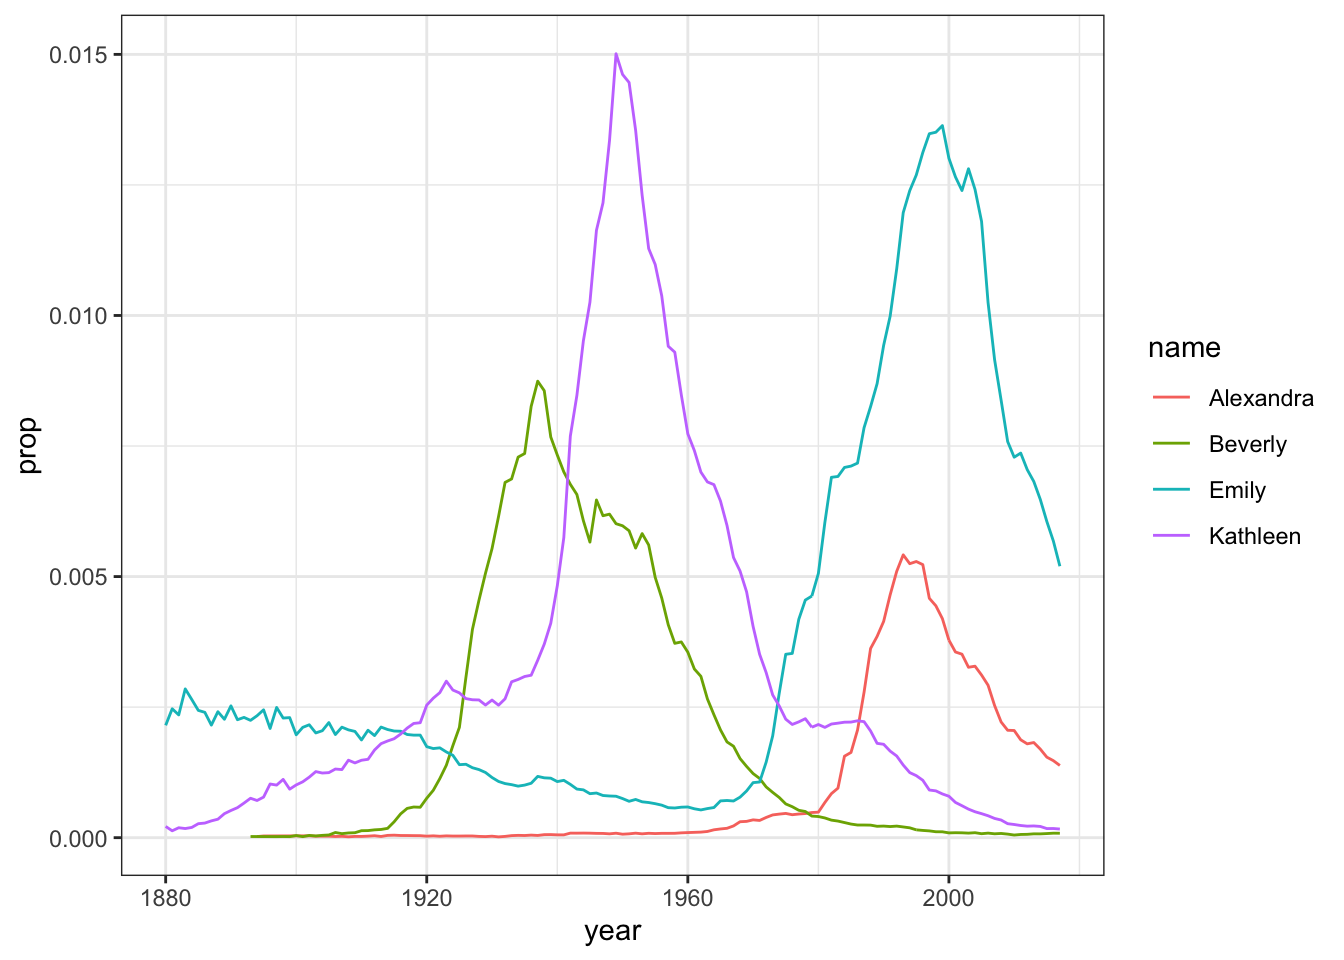
\includegraphics[width=1\linewidth]{05-wrangling-1_files/figure-latex/babynames-plot-1} 

}

\caption{Proportion of four baby names from 1880 to 2014}\label{fig:babynames-plot}
\end{figure}

\begin{itemize}
\tightlist
\item
  Change the names to your own examples and see how the plot changes. You can also change the sex from ``F'' to ``M''. Post the photos of your new plots on the Teams Data Skills channel.
\item
  Because in most countries assigned sex at birth is binary, there is no data on intersex, trans or non-binary names. In lieu of that, here's the \href{https://en.wikipedia.org/wiki/Unisex_name}{Wikipedia page about gender-neutral names and naming laws} around the world which will hopefully make you question why on earth we ascribe someone's entire gender identity to a bunch of sounds and letters we use to label them.
\end{itemize}

But I want to display male AND female names!

This is more complicated than you might first imagine so only read on if you're feeling confident. If you remove the filter for \texttt{sex} when creating \texttt{dat} and then run the plot code again, it will make a very messy looking plot (try it). This is because for most names there will be two data points because although the numbers might be small for gendered names, there is usually always at least one baby of the non-dominant name gender that has been assigned that name.

You can get around this by adding an additional line of code that produces separate plots by sex. The scale argument tells R that it can use different scales on the y-axis for each plot - when there's a large difference between the two scales this is helpful to allow you to see the data in both sets (run this code and then remove the scales argument and run it again to see the difference) although it does run the risk of people misinterpreting the data if the difference between the scales isn't made clear.

\begin{Shaded}
\begin{Highlighting}[]
\NormalTok{dat2 }\OtherTok{\textless{}{-}}\NormalTok{ babynames }\SpecialCharTok{\%\textgreater{}\%} 
  \FunctionTok{filter}\NormalTok{(name }\SpecialCharTok{\%in\%} \FunctionTok{c}\NormalTok{(}\StringTok{"Emily"}\NormalTok{,}\StringTok{"Kathleen"}\NormalTok{,}\StringTok{"Alexandra"}\NormalTok{,}\StringTok{"Beverly"}\NormalTok{))}

\FunctionTok{ggplot}\NormalTok{(}\AttributeTok{data =}\NormalTok{ dat2,}\FunctionTok{aes}\NormalTok{(}\AttributeTok{x =}\NormalTok{ year,}\AttributeTok{y =}\NormalTok{ prop, }\AttributeTok{colour=}\NormalTok{name))}\SpecialCharTok{+}
  \FunctionTok{geom\_line}\NormalTok{() }\SpecialCharTok{+}
  \FunctionTok{facet\_wrap}\NormalTok{(}\SpecialCharTok{\textasciitilde{}}\NormalTok{sex, }\AttributeTok{scales =} \StringTok{"free\_y"}\NormalTok{, }\AttributeTok{nrow =} \DecValTok{2}\NormalTok{)}
\end{Highlighting}
\end{Shaded}

\begin{figure}

{\centering \includegraphics[width=1\linewidth]{05-wrangling-1_files/figure-latex/unnamed-chunk-4-1} 

}

\caption{Plots by sex with different scales}\label{fig:unnamed-chunk-4}
\end{figure}

On the other hand, if the scales for your two groups are fairly similar, it's better to keep the same scales to aid comparison. This time we will filter the dataset for gender neutral names where it might make more sense to have them on the same scale - again try it with and without the scales argument to see what happens

\begin{Shaded}
\begin{Highlighting}[]
\NormalTok{dat3 }\OtherTok{\textless{}{-}}\NormalTok{ babynames }\SpecialCharTok{\%\textgreater{}\%} 
  \FunctionTok{filter}\NormalTok{(name }\SpecialCharTok{\%in\%} \FunctionTok{c}\NormalTok{(}\StringTok{"Sam"}\NormalTok{,}\StringTok{"Alex"}\NormalTok{,}\StringTok{"Jordan"}\NormalTok{,}\StringTok{"Drew"}\NormalTok{))}

\FunctionTok{ggplot}\NormalTok{(}\AttributeTok{data =}\NormalTok{ dat3,}\FunctionTok{aes}\NormalTok{(}\AttributeTok{x =}\NormalTok{ year,}\AttributeTok{y =}\NormalTok{ prop, }\AttributeTok{colour=}\NormalTok{name))}\SpecialCharTok{+}
  \FunctionTok{geom\_line}\NormalTok{() }\SpecialCharTok{+}
  \FunctionTok{facet\_wrap}\NormalTok{(}\SpecialCharTok{\textasciitilde{}}\NormalTok{sex, }\AttributeTok{nrow =} \DecValTok{2}\NormalTok{)}
\end{Highlighting}
\end{Shaded}

\begin{figure}

{\centering \includegraphics[width=1\linewidth]{05-wrangling-1_files/figure-latex/unnamed-chunk-5-1} 

}

\caption{Plots by sex with the same scale}\label{fig:unnamed-chunk-5}
\end{figure}

\hypertarget{activity-4-selecting-variables-of-interest}{%
\section{Activity 4: Selecting variables of interest}\label{activity-4-selecting-variables-of-interest}}

There are two numeric measurements of name popularity, \texttt{prop} (the proportion of all babies with each name) is probably more useful than \texttt{n} (total number of babies with that name), because it takes into account that different numbers of babies are born in different years.

Just like in Loading Data, if we wanted to create a dataset that only includes certain variables, we can use the \texttt{select()} function from the \texttt{dplyr} package. Run the below code to only select the columns \texttt{year}, \texttt{sex}, \texttt{name} and \texttt{prop}.

\begin{Shaded}
\begin{Highlighting}[]
\FunctionTok{select}\NormalTok{(}\AttributeTok{.data =}\NormalTok{ babynames, }\CommentTok{\# the object you want to select variables from}
\NormalTok{       year, sex, name, prop) }\CommentTok{\# the variables you want to select}
\end{Highlighting}
\end{Shaded}

\begin{danger}
If you get an error message when using select that says
\texttt{unused\ argument} it means that it is trying to use the wrong
version of the select function. There are two solutions to this, first,
save you work and then restart the R session (click session -restart R)
and then run all your code above again from the start, or replace
\texttt{select} with \texttt{dplyr::select} which tells R exactly which
version of the select function to use. We'd recommend restarting the
session because this will get you in the habit and it's a useful thing
to try for a range of problems
\end{danger}

Alternatively, you can also tell R which variables you don't want, in this case, rather than telling R to select \texttt{year}, \texttt{sex}, \texttt{name} and \texttt{prop}, we can simply tell it to drop the column \texttt{n} using the minus sign \texttt{-} before the variable name.

\begin{Shaded}
\begin{Highlighting}[]
\FunctionTok{select}\NormalTok{(}\AttributeTok{.data =}\NormalTok{ babynames, }\SpecialCharTok{{-}}\NormalTok{n)}
\end{Highlighting}
\end{Shaded}

Note that \texttt{select()} does not change the original tibble, but makes a new tibble with the specified columns. If you don't save this new tibble to an object, it won't be saved. If you want to keep this new dataset, create a new object. When you run this code, you will see your new tibble appear in the environment pane.

\begin{Shaded}
\begin{Highlighting}[]
\NormalTok{new\_dat }\OtherTok{\textless{}{-}} \FunctionTok{select}\NormalTok{(}\AttributeTok{.data =}\NormalTok{ babynames, }\SpecialCharTok{{-}}\NormalTok{n)}
\end{Highlighting}
\end{Shaded}

\hypertarget{activity-5-arranging-the-data}{%
\section{Activity 5: Arranging the data}\label{activity-5-arranging-the-data}}

The function \texttt{arrange()} will sort the rows in the table according to the columns you supply. Try running the following code:

\begin{Shaded}
\begin{Highlighting}[]
\FunctionTok{arrange}\NormalTok{(}\AttributeTok{.data =}\NormalTok{ babynames, }\CommentTok{\# the data you want to sort}
\NormalTok{        name) }\CommentTok{\# the variable you want to sort by}
\end{Highlighting}
\end{Shaded}

The data are now sorted in ascending alphabetical order by name. The default is to sort in ascending order. If you want it descending, wrap the name of the variable in the \texttt{desc()} function. For instance, to sort by year in descending order, run the following code:

\begin{Shaded}
\begin{Highlighting}[]
\FunctionTok{arrange}\NormalTok{(babynames,}\FunctionTok{desc}\NormalTok{(year)) }
\end{Highlighting}
\end{Shaded}

You can also sort by more than one column. What do you think the following code will do?

\begin{Shaded}
\begin{Highlighting}[]
\FunctionTok{arrange}\NormalTok{(babynames, }\FunctionTok{desc}\NormalTok{(year), }\FunctionTok{desc}\NormalTok{(sex), }\FunctionTok{desc}\NormalTok{(prop)) }
\end{Highlighting}
\end{Shaded}

\hypertarget{activity-6-using-filter-to-select-observations}{%
\section{Activity 6: Using filter to select observations}\label{activity-6-using-filter-to-select-observations}}

We have previously used \texttt{select()} to select certain variables or columns, however, frequently you will also want to select only certain observations or rows, for example, only babies born after 1999, or only babies named ``Mary''. You do this using the verb \texttt{filter()}. The \texttt{filter()} function is a bit more involved than the other verbs, and requires more detailed explanation, but this is because it is also extremely powerful.

Here is an example of filter, can you guess what it will do?

\begin{Shaded}
\begin{Highlighting}[]
 \FunctionTok{filter}\NormalTok{(}\AttributeTok{.data =}\NormalTok{ babynames, year }\SpecialCharTok{\textgreater{}} \DecValTok{2000}\NormalTok{)}
\end{Highlighting}
\end{Shaded}

The first part of the code tells the function to use the object \texttt{babynames}. The second argument, \texttt{year\ \textgreater{}\ 2000}, is what is known as a \textbf{Boolean expression}: an expression whose evaluation results in a value of TRUE or FALSE. What \texttt{filter()} does is include any observations (rows) for which the expression evaluates to TRUE, and exclude any for which it evaluates to FALSE. So in effect, behind the scenes, \texttt{filter()} goes through the entire set of 1.8 million observations, row by row, checking the value of year for each row, keeping it if the value is greater than 2000, and rejecting it if it is less than 2000. To see how a boolean expression works, consider the code below:

\begin{Shaded}
\begin{Highlighting}[]
\NormalTok{years }\OtherTok{\textless{}{-}} \DecValTok{1996}\SpecialCharTok{:}\DecValTok{2005}
\NormalTok{years}
\NormalTok{years }\SpecialCharTok{\textgreater{}} \DecValTok{2000}
\end{Highlighting}
\end{Shaded}

\begin{verbatim}
##  [1] 1996 1997 1998 1999 2000 2001 2002 2003 2004 2005
##  [1] FALSE FALSE FALSE FALSE FALSE  TRUE  TRUE  TRUE  TRUE  TRUE
\end{verbatim}

You can see that the expression \texttt{years\ \textgreater{}\ 2000} returns a \textbf{logical vector} (a vector of TRUE and FALSE values), where each element represents whether the expression is true or false for that element. For the first five elements (1996 to 2000) it is false, and for the last five elements (2001 to 2005) it is true.

Here are the most commonly used Boolean expressions.

\begin{longtable}[]{@{}lll@{}}
\toprule
Operator & Name & is TRUE if and only if \\
\midrule
\endhead
A \textless{} B & less than & A is less than B \\
A \textless= B & less than or equal & A is less than or equal to B \\
A \textgreater{} B & greater than & A is greater than B \\
A \textgreater= B & greater than or equal & A is greater than or equal to B \\
A == B & equivalence & A exactly equals B \\
A != B & not equal & A does not exactly equal B \\
A \%in\% B & in & A is an element of vector B \\
\bottomrule
\end{longtable}

If you want only those observations for a specific name (e.g., Mary), you use the equivalence operator \texttt{==}. Note that you use double equal signs, not a single equal sign.

\begin{Shaded}
\begin{Highlighting}[]
\FunctionTok{filter}\NormalTok{(babynames, name }\SpecialCharTok{==} \StringTok{"Mary"}\NormalTok{)}
\end{Highlighting}
\end{Shaded}

If you wanted all the names except Mary, you use the `not equals' operator:

\begin{Shaded}
\begin{Highlighting}[]
\FunctionTok{filter}\NormalTok{(babynames, name}\SpecialCharTok{!=}\StringTok{"Mary"}\NormalTok{) }
\end{Highlighting}
\end{Shaded}

And if you wanted names from a defined set - e.g., names of British queens - you can use \texttt{\%in\%}:

\begin{Shaded}
\begin{Highlighting}[]
\FunctionTok{filter}\NormalTok{(babynames, name }\SpecialCharTok{\%in\%} \FunctionTok{c}\NormalTok{(}\StringTok{"Mary"}\NormalTok{,}\StringTok{"Elizabeth"}\NormalTok{,}\StringTok{"Victoria"}\NormalTok{))}
\end{Highlighting}
\end{Shaded}

This gives you data for the names in the vector on the right hand side of \texttt{\%in\%}. You can always invert an expression to get its opposite. So, for instance, if you instead wanted to get rid of all Marys, Elizabeths, and Victorias you would use the following:

\begin{Shaded}
\begin{Highlighting}[]
\FunctionTok{filter}\NormalTok{(babynames, }\SpecialCharTok{!}\NormalTok{(name }\SpecialCharTok{\%in\%} \FunctionTok{c}\NormalTok{(}\StringTok{"Mary"}\NormalTok{,}\StringTok{"Elizabeth"}\NormalTok{,}\StringTok{"Victoria"}\NormalTok{)))}
\end{Highlighting}
\end{Shaded}

You can include as many expressions as you like as additional arguments to \texttt{filter()} and it will only pull out the rows for which all of the expressions for that row evaluate to TRUE. For instance, \texttt{filter(babynames,\ year\ \textgreater{}\ 2000,\ prop\ \textgreater{}\ .01)} will pull out only those observations beyond the year 2000 that represent greater than 1\% of the names for a given sex; any observation where either expression is false will be excluded. This ability to string together criteria makes \texttt{filter()} a very powerful member of the Wickham Six.

\textbf{Remember that this section exists. It will contain a lot of the answers to problems you face when wrangling data!}

\hypertarget{activity-7-creating-new-variables}{%
\section{Activity 7: Creating new variables}\label{activity-7-creating-new-variables}}

Sometimes we need to create a new variable that doesn't exist in our dataset. For instance, we might want to figure out what decade a particular year belongs to. To create new variables, we use the function \texttt{mutate()}. Note that if you want to save this new column, you need to save it to an object. Here, you are mutating a new column and attaching it to the \texttt{new\_dat} object you created in Activity 4.

\begin{Shaded}
\begin{Highlighting}[]
\NormalTok{new\_dat }\OtherTok{\textless{}{-}} \FunctionTok{mutate}\NormalTok{(}\AttributeTok{.data =}\NormalTok{ babynames, }\CommentTok{\# the tibble you want to add a column to}
                  \AttributeTok{decade =} \FunctionTok{floor}\NormalTok{(year}\SpecialCharTok{/}\DecValTok{10}\NormalTok{) }\SpecialCharTok{*}\DecValTok{10}\NormalTok{) }\CommentTok{\# new column name = what you want it to contain}
\FunctionTok{head}\NormalTok{(new\_dat)}
\end{Highlighting}
\end{Shaded}

\begin{verbatim}
## # A tibble: 6 x 6
##    year sex   name          n   prop decade
##   <dbl> <chr> <chr>     <int>  <dbl>  <dbl>
## 1  1880 F     Mary       7065 0.0724   1880
## 2  1880 F     Anna       2604 0.0267   1880
## 3  1880 F     Emma       2003 0.0205   1880
## 4  1880 F     Elizabeth  1939 0.0199   1880
## 5  1880 F     Minnie     1746 0.0179   1880
## 6  1880 F     Margaret   1578 0.0162   1880
\end{verbatim}

In this case, you are creating a new column decade which has the decade each year appears in. This is calculated using the command \texttt{decade\ =\ floor(year/10)*10}.

\hypertarget{activity-8-grouping-and-summarising}{%
\section{Activity 8: Grouping and summarising}\label{activity-8-grouping-and-summarising}}

Most quantitative analyses will require you to summarise your data somehow, for example, by calculating the mean, median or a sum total of your data. You can perform all of these operations using the function \texttt{summarise()}.

First, let's use the object \texttt{dat} that just has the data for the four girls names, Alexandra, Beverly, Emily, and Kathleen. To start off, we're simply going to calculate the total number of babies across all years that were given one of these four names.

It's useful to get in the habit of translating your code into full sentences to make it easier to figure out what's happening. You can read the below code as ``run the function summarise using the data in the object \texttt{dat} to create a new variable named \texttt{total} that is the result of adding up all the numbers in the column \texttt{n}''.

\begin{Shaded}
\begin{Highlighting}[]
\FunctionTok{summarise}\NormalTok{(}\AttributeTok{.data =}\NormalTok{ dat, }\CommentTok{\# the data you want to use}
          \AttributeTok{total =} \FunctionTok{sum}\NormalTok{(n)) }\CommentTok{\# result = operation}
\end{Highlighting}
\end{Shaded}

\begin{verbatim}
## # A tibble: 1 x 1
##     total
##     <int>
## 1 2161374
\end{verbatim}

\texttt{summarise()} becomes even more powerful when combined with the final \texttt{dplyr} function, \texttt{group\_by()}. Quite often, you will want to produce your summary statistics broken down by groups, for examples, the scores of participants in different conditions, or the reading time for native and non-native speakers.

There are two ways you can use \texttt{group\_by()}. First, you can create a new, grouped object.

\begin{Shaded}
\begin{Highlighting}[]
\NormalTok{group\_dat }\OtherTok{\textless{}{-}} \FunctionTok{group\_by}\NormalTok{(}\AttributeTok{.data =}\NormalTok{ dat, }\CommentTok{\# the data you want to group}
\NormalTok{                      name) }\CommentTok{\# the variable you want to group by}
\end{Highlighting}
\end{Shaded}

If you look at this object in the viewer, it won't look any different to the original \texttt{dat}, however, the underlying structure has changed. Let's run the above summarise code again, but now using the grouped data.

\begin{Shaded}
\begin{Highlighting}[]
\FunctionTok{summarise}\NormalTok{(}\AttributeTok{.data =}\NormalTok{ group\_dat, }
          \AttributeTok{total =} \FunctionTok{sum}\NormalTok{(n)) }
\end{Highlighting}
\end{Shaded}

\begin{verbatim}
## # A tibble: 4 x 2
##   name       total
##   <chr>      <int>
## 1 Alexandra 231364
## 2 Beverly   376914
## 3 Emily     841491
## 4 Kathleen  711605
\end{verbatim}

\texttt{summarise()} has performed exactly the same operation as before - adding up the total number in the column \texttt{n} - but this time it has done is separately for each group, which in this case was the variable \texttt{name}.

You can request multiple summary calculations to be performed in the same function. For example, the following code calculates the mean and median number of babies given each name every year.

\begin{Shaded}
\begin{Highlighting}[]
\FunctionTok{summarise}\NormalTok{(group\_dat,}
          \AttributeTok{mean\_year =} \FunctionTok{mean}\NormalTok{(n),}
          \AttributeTok{median\_year =} \FunctionTok{median}\NormalTok{(n))}
\end{Highlighting}
\end{Shaded}

\begin{verbatim}
## # A tibble: 4 x 3
##   name      mean_year median_year
##   <chr>         <dbl>       <dbl>
## 1 Alexandra     1977.        192 
## 2 Beverly       3089.        710.
## 3 Emily         6098.       1392.
## 4 Kathleen      5157.       3098
\end{verbatim}

You can also add multiple grouping variables. For example, the following code groups \texttt{new\_dat} by \texttt{sex} and \texttt{decade} and then calculates the summary statistics to give us the mean and median number of male and female babies in each decade.

\begin{Shaded}
\begin{Highlighting}[]
\NormalTok{group\_new\_dat }\OtherTok{\textless{}{-}} \FunctionTok{group\_by}\NormalTok{(new\_dat, sex, decade)}
\FunctionTok{summarise}\NormalTok{(group\_new\_dat,}
          \AttributeTok{mean\_year =} \FunctionTok{mean}\NormalTok{(n),}
          \AttributeTok{median\_year =} \FunctionTok{median}\NormalTok{(n))}
\end{Highlighting}
\end{Shaded}

\begin{verbatim}
## `summarise()` has grouped output by 'sex'. You can override using the `.groups` argument.
\end{verbatim}

\begin{verbatim}
## # A tibble: 28 x 4
## # Groups:   sex [2]
##    sex   decade mean_year median_year
##    <chr>  <dbl>     <dbl>       <dbl>
##  1 F       1880      111.          13
##  2 F       1890      128.          13
##  3 F       1900      131.          12
##  4 F       1910      187.          12
##  5 F       1920      211.          12
##  6 F       1930      214.          12
##  7 F       1940      262.          12
##  8 F       1950      288.          13
##  9 F       1960      235.          12
## 10 F       1970      147.          11
## # ... with 18 more rows
\end{verbatim}

\begin{info}
If you get what looks like an error that says
\texttt{summarise()\ ungrouping\ output\ (override\ with\ .groups\ argument)}don't
worry, this isn't an error it's just R telling you what it's done. This
message was included in a very recent update to the \texttt{tidyverse}
which is why it doesn't appear on some of the walkthrough vidoes.
\end{info}

\hypertarget{activity-9-pipes}{%
\section{Activity 9: Pipes}\label{activity-9-pipes}}

The final activity for this chapter essentially repeats what we've already covered but in a slightly different way. In the previous activities, you created new objects with new variables or groupings and then you called \texttt{summarise()} on those new objects in separate lines of code. As a result, you had multiple objects in your environment pane and you need to make sure that you keep track of the different names.

Instead, you can use \textbf{pipes}. Pipes are written as \texttt{\%\textgreater{}\%}and they should be read as ``and then''. Pipes allow you to string together `sentences' of code into `paragraphs' so that you don't need to create intermediary objects. Again, it is easier to show than tell.

The below code does \textbf{exactly} the same as all the code we wrote above but it only creates one object.

\begin{Shaded}
\begin{Highlighting}[]
\NormalTok{pipe\_summary }\OtherTok{\textless{}{-}} \FunctionTok{mutate}\NormalTok{(babynames, }\AttributeTok{decade =} \FunctionTok{floor}\NormalTok{(year}\SpecialCharTok{/}\DecValTok{10}\NormalTok{) }\SpecialCharTok{*}\DecValTok{10}\NormalTok{) }\SpecialCharTok{\%\textgreater{}\%}
  \FunctionTok{filter}\NormalTok{(name }\SpecialCharTok{\%in\%} \FunctionTok{c}\NormalTok{(}\StringTok{"Emily"}\NormalTok{,}\StringTok{"Kathleen"}\NormalTok{,}\StringTok{"Alexandra"}\NormalTok{,}\StringTok{"Beverly"}\NormalTok{), sex}\SpecialCharTok{==}\StringTok{"F"}\NormalTok{) }\SpecialCharTok{\%\textgreater{}\%}
  \FunctionTok{group\_by}\NormalTok{(name, decade) }\SpecialCharTok{\%\textgreater{}\%}
  \FunctionTok{summarise}\NormalTok{(}\AttributeTok{mean\_decade =} \FunctionTok{mean}\NormalTok{(n))}
\end{Highlighting}
\end{Shaded}

The reason that this function is called a pipe is because it `pipes' the data through to the next function. When you wrote the code previously, the first argument of each function was the dataset you wanted to work on. When you use pipes it will automatically take the data from the previous line of code so you don't need to specify it again.

\begin{try}
When learning to code it can be a useful practice to read your code `out
loud' in full sentences to help you understand what it is doing. You can
read the code above as ``create a new variable called decade AND THEN
only keep the names Emily, Kathleen, Alexandra and Beverly that belong
to female babies AND THEN group the dataset by name and decade AND THEN
calculate the mean number of babies with each name per decade.'' Try
doing this each time you write a new bit of code.
\end{try}

Some people find pipes a bit tricky to understand from a conceptual point of view, however, it's well worth learning to use them as when your code starts getting longer they are much more efficient and mean you have to write less code which is always a good thing!

\hypertarget{finished-2}{%
\section{Finished!}\label{finished-2}}

That was a long chapter but remember, you don't need to memorise all of this code. You just need to know where to look for help. Finally, if you're working from the R server, we'd recommend that you download a copy of the changes you've made to \texttt{stub-wrangling-1} so that you have a backup.

\hypertarget{data-wrangling-2}{%
\chapter{Data wrangling 2}\label{data-wrangling-2}}

\hypertarget{walkthrough-video-3}{%
\section{Walkthrough video}\label{walkthrough-video-3}}

There is a \href{https://uofglasgow.zoom.us/rec/play/Kde7hTS2bAJAvhuAufvxpYi8shgfoSH4kKeWN8YGJ9k1_lbHDFsNzHZBm9Bfu_bKVtcOxoNQbrBf8Ddt.Cy_Kex6M9v1_3v_G?startTime=1602841645000\&_x_zm_rtaid=cW5f8v0JQcOlLI1cBpI84g.1628694791961.c3bcc75dbabdfb3f3ac44f8fd7884865\&_x_zm_rhtaid=355}{walkthrough video} of this chapter available via Zoom.

\begin{itemize}
\tightlist
\item
  Video notes: this video was recorded in 2020, it uses the server, and the book has been updated visually. There are no other differences between the video and this book chapter.
\end{itemize}

\hypertarget{activity-1-set-up-2}{%
\section{Activity 1: Set-up}\label{activity-1-set-up-2}}

\begin{itemize}
\tightlist
\item
  Open R Studio and ensure the environment is clear.\\
\item
  Open the \texttt{stub-wrangling-2.Rmd} file and ensure that the working directory is set to your Data Skills folder and that the two .csv data files (\texttt{participant-info.csv} and \texttt{ahi-cesd.csv}) are in your working directory (you should see them in the file pane).\\
\item
  If you're on the server, avoid a number of issues by restarting the session - click \texttt{Session} - \texttt{Restart\ R}\\
\item
  Type and run the below code to load the \texttt{tidyverse} package and to load in the data files.
\end{itemize}

\begin{Shaded}
\begin{Highlighting}[]
\FunctionTok{library}\NormalTok{(tidyverse) }

\NormalTok{dat }\OtherTok{\textless{}{-}} \FunctionTok{read\_csv}\NormalTok{(}\StringTok{\textquotesingle{}ahi{-}cesd.csv\textquotesingle{}}\NormalTok{)}
\NormalTok{pinfo }\OtherTok{\textless{}{-}} \FunctionTok{read\_csv}\NormalTok{(}\StringTok{\textquotesingle{}participant{-}info.csv\textquotesingle{}}\NormalTok{)}
\NormalTok{all\_dat }\OtherTok{\textless{}{-}} \FunctionTok{inner\_join}\NormalTok{(dat, pinfo, }\AttributeTok{by=} \FunctionTok{c}\NormalTok{(}\StringTok{"id"}\NormalTok{, }\StringTok{"intervention"}\NormalTok{))}
\end{Highlighting}
\end{Shaded}

Now let's start working with our \texttt{tidyverse} verb functions\ldots{}

\hypertarget{activity-2-select}{%
\section{Activity 2: Select}\label{activity-2-select}}

Select the columns all\_dat, ahiTotal, cesdTotal, sex, age, educ, income, occasion, elapsed.days from the data and create a variable called \texttt{summarydata}.

\begin{Shaded}
\begin{Highlighting}[]
\NormalTok{summarydata }\OtherTok{\textless{}{-}} \FunctionTok{select}\NormalTok{(all\_dat, ahiTotal, cesdTotal, sex, age, educ, income, occasion, elapsed.days)}
\end{Highlighting}
\end{Shaded}

\begin{danger}
If you get an error message when using select that says
\texttt{unused\ argument} it means that it is trying to use the wrong
version of the select function. There are two solutions to this, first,
save you work and then restart the R session (click session -restart R)
and then run all your code above again from the start, or replace
\texttt{select} with \texttt{dplyr::select} which tells R exactly which
version of the select function to use. We'd recommend restarting the
session because this will get you in the habit and it's a useful thing
to try for a range of problems
\end{danger}

\begin{center}\rule{0.5\linewidth}{0.5pt}\end{center}

\textbf{Pause here and interpret the above code and output}

\begin{itemize}
\tightlist
\item
  How you would translate this code into English
\item
  What columns have been removed from the data?
\end{itemize}

\begin{center}\rule{0.5\linewidth}{0.5pt}\end{center}

\hypertarget{activity-3-arrange}{%
\section{Activity 3: Arrange}\label{activity-3-arrange}}

Arrange the data in the variable created above (\texttt{summarydata}) by ahiTotal with lowest score first.

\begin{Shaded}
\begin{Highlighting}[]
\NormalTok{ahi\_asc }\OtherTok{\textless{}{-}} \FunctionTok{arrange}\NormalTok{(summarydata, }\AttributeTok{by =}\NormalTok{ ahiTotal)}
\end{Highlighting}
\end{Shaded}

\begin{center}\rule{0.5\linewidth}{0.5pt}\end{center}

\begin{itemize}
\tightlist
\item
  How could you arrange this data in \textbf{descending} order (highest score first)?
\end{itemize}

Solution

\begin{Shaded}
\begin{Highlighting}[]
\FunctionTok{arrange}\NormalTok{(summarydata, }\AttributeTok{by =} \FunctionTok{desc}\NormalTok{(ahiTotal))}
\end{Highlighting}
\end{Shaded}

\begin{itemize}
\item
  What is the smallest ahiTotal score?
\item
  What is the largest ahiTotal score?
\end{itemize}

\begin{center}\rule{0.5\linewidth}{0.5pt}\end{center}

\hypertarget{activity-4-filter}{%
\section{Activity 4: Filter}\label{activity-4-filter}}

Filter the data \texttt{ahi\_asc} by taking out those who are over 65 years of age.

\begin{Shaded}
\begin{Highlighting}[]
\NormalTok{age\_65max }\OtherTok{\textless{}{-}} \FunctionTok{filter}\NormalTok{(ahi\_asc, age }\SpecialCharTok{\textless{}} \DecValTok{65}\NormalTok{)}
\end{Highlighting}
\end{Shaded}

\begin{center}\rule{0.5\linewidth}{0.5pt}\end{center}

\begin{itemize}
\tightlist
\item
  What does \texttt{filter()} do?
\end{itemize}

splits a column into multiple columnstransforms existing columnstakes multiple columns and collapses them togetherremoves information that we are not interested in

\begin{itemize}
\tightlist
\item
  How many observations are left in \texttt{age\_65max} after running \texttt{filter()}?
\end{itemize}

\begin{center}\rule{0.5\linewidth}{0.5pt}\end{center}

\hypertarget{activity-5-summarise}{%
\section{Activity 5: Summarise}\label{activity-5-summarise}}

Then, use summarise to create a new variable \texttt{data\_median}, which calculates the median ahiTotal score in this grouped data and assign it a table head called \texttt{median\_score}.

\begin{Shaded}
\begin{Highlighting}[]
\NormalTok{data\_median }\OtherTok{\textless{}{-}} \FunctionTok{summarise}\NormalTok{(age\_65max, }\AttributeTok{median\_score =} \FunctionTok{median}\NormalTok{(ahiTotal))}
\end{Highlighting}
\end{Shaded}

\begin{center}\rule{0.5\linewidth}{0.5pt}\end{center}

\begin{itemize}
\item
  What is the median score?
\item
  Change the above code to give you the \textbf{mean score}. What is the mean score to 2 decimal places?
\end{itemize}

Solution

\begin{Shaded}
\begin{Highlighting}[]
\FunctionTok{summarise}\NormalTok{(age\_65max, }\AttributeTok{mean\_score =} \FunctionTok{mean}\NormalTok{(ahiTotal))}
\end{Highlighting}
\end{Shaded}

\begin{center}\rule{0.5\linewidth}{0.5pt}\end{center}

\hypertarget{activity-6-group_by}{%
\section{Activity 6: Group\_by}\label{activity-6-group_by}}

Use mutate to create a new column called \texttt{Happiness\_Category} in \texttt{age\_65max} which categorises participants based on whether they score above the median \texttt{ahiTotal} score for all participants.

Then, group the data stored in \texttt{age\_65max} by \texttt{Happiness\_Category}, and store it in an object named \texttt{happy\_dat}.

Finally, use summarise to calculate the median \texttt{cesdTotal} score for participants who scored above and below the median \texttt{ahiTotal} score and save it in a new object named \texttt{data\_median\_group}.

\begin{Shaded}
\begin{Highlighting}[]
\NormalTok{age\_65max }\OtherTok{\textless{}{-}} \FunctionTok{mutate}\NormalTok{(age\_65max, }\AttributeTok{Happiness\_Category =}\NormalTok{ (ahiTotal }\SpecialCharTok{\textgreater{}} \DecValTok{74}\NormalTok{))}
\NormalTok{happy\_dat }\OtherTok{\textless{}{-}} \FunctionTok{group\_by}\NormalTok{(age\_65max, Happiness\_Category)}

\NormalTok{data\_median\_group }\OtherTok{\textless{}{-}} \FunctionTok{summarise}\NormalTok{(happy\_dat, }\AttributeTok{median\_score =} \FunctionTok{median}\NormalTok{(cesdTotal))}
\end{Highlighting}
\end{Shaded}

\begin{info}
If you get what looks like an error that says
\texttt{summarise()\ ungrouping\ output\ (override\ with\ .groups\ argument)}don't
worry, this isn't an error it's just R telling you what it's done. This
message was included in a very recent update to the \texttt{tidyverse}
which is why it doesn't appear on some of the walkthrough vidoes.
\end{info}

\begin{center}\rule{0.5\linewidth}{0.5pt}\end{center}

\textbf{Pause here and interpret the above code and output}

\begin{itemize}
\tightlist
\item
  What does \texttt{group\_by()} do?
\end{itemize}

provides summary statistics of an existing dataframeorganises information in ascending or descending ordertransforms existing columnsgroups data frames based on a specific column so that all later operations are carried out on a group basis

\begin{itemize}
\tightlist
\item
  How would you change the code to group by education rather than \texttt{Happiness\_Category}?
\end{itemize}

Solution

\begin{Shaded}
\begin{Highlighting}[]
\FunctionTok{group\_by}\NormalTok{(age\_65max, educ)}
\end{Highlighting}
\end{Shaded}

\begin{center}\rule{0.5\linewidth}{0.5pt}\end{center}

\hypertarget{activity-7-data-visualisation}{%
\section{Activity 7: Data visualisation}\label{activity-7-data-visualisation}}

Copy, paste and run the below code into a new code chunk to create a plot of depression scores grouped by income level using the \texttt{age\_65max} data.

\begin{Shaded}
\begin{Highlighting}[]
\FunctionTok{ggplot}\NormalTok{(age\_65max, }\FunctionTok{aes}\NormalTok{(}\AttributeTok{x =} \FunctionTok{as.factor}\NormalTok{(income), }\AttributeTok{y =}\NormalTok{ cesdTotal, }\AttributeTok{fill =} \FunctionTok{as.factor}\NormalTok{(income))) }\SpecialCharTok{+}
  \FunctionTok{geom\_violin}\NormalTok{(}\AttributeTok{trim =} \ConstantTok{FALSE}\NormalTok{, }\AttributeTok{show.legend =} \ConstantTok{FALSE}\NormalTok{, }\AttributeTok{alpha =}\NormalTok{ .}\DecValTok{6}\NormalTok{) }\SpecialCharTok{+}
  \FunctionTok{geom\_boxplot}\NormalTok{(}\AttributeTok{width =}\NormalTok{ .}\DecValTok{2}\NormalTok{, }\AttributeTok{show.legend =} \ConstantTok{FALSE}\NormalTok{, }\AttributeTok{alpha =}\NormalTok{ .}\DecValTok{5}\NormalTok{) }\SpecialCharTok{+}
  \FunctionTok{scale\_fill\_viridis\_d}\NormalTok{(}\AttributeTok{option =} \StringTok{"D"}\NormalTok{) }\SpecialCharTok{+}
  \FunctionTok{scale\_x\_discrete}\NormalTok{(}\AttributeTok{name =} \StringTok{"Income Level"}\NormalTok{, }\AttributeTok{labels =} \FunctionTok{c}\NormalTok{(}\StringTok{"Below Average"}\NormalTok{, }\StringTok{"Average"}\NormalTok{, }\StringTok{"Above Average"}\NormalTok{)) }\SpecialCharTok{+}
  \FunctionTok{scale\_y\_continuous}\NormalTok{(}\AttributeTok{name =} \StringTok{"Depression Score"}\NormalTok{)}
\end{Highlighting}
\end{Shaded}

\begin{itemize}
\item
  Which income group has the highest median depression scores? Below AverageAverageAbove Average
\item
  Which group has the highest density of scores at any one point? Below AverageAverageAbove Average
\end{itemize}

Explain This Answer

Density is represented by the curvy line around the boxplot that looks a little bit like a (drunk) violin. The fatter the violin, the more data points there are at any one point. This means that in the above plot, the Above Average group has the highest density because this has the widest violin, i.e., there are lots of people in the Above Average income group with a score of about 5.

\begin{itemize}
\tightlist
\item
  Is income group a between-subject or within-subject variable? Between-subjectsWithin-subjects
\end{itemize}

Explain This Answer

Between-subjects designs are where different participants are in different groups. Within-subject designs are when the same participants are in all groups. Income is an example of a between-subject variable because participants can only be in one grouping level of the independent variable

\hypertarget{activity-8-make-r-your-own}{%
\section{Activity 8: Make R your own}\label{activity-8-make-r-your-own}}

Finally, you can customise how R Studio looks to make it feel more like your own personal version. Click \texttt{Tools} - \texttt{Global\ Options} - \texttt{Apperance}. You can change the default font, font size, and general appearance of R Studio, including using dark mode. Play around with the settings and see which one you prefer - you're going to spend a lot of time with R, it might as well look nice!

\hypertarget{finished-3}{%
\section{Finished!}\label{finished-3}}

Well done! As a final step, try knitting the file to HTML. Remember to save your Markdown in your Data Skills folder and make a note of any mistakes you made and how you fixed them.

\hypertarget{intro-to-data-viz}{%
\chapter{Intro to Data Viz}\label{intro-to-data-viz}}

\hypertarget{walkthrough-video-4}{%
\section{Walkthrough video}\label{walkthrough-video-4}}

There is a \href{https://uofglasgow.zoom.us/rec/play/Q9BA93fhXCTrTyRF962J8cWI7YDQ1dca0u3sbPstj-ktY4e52jv_b5vtAZMgI6fAM3Cip_L0itlsym8.zF0_1My59xl1MGmG?startTime=1602848670000\&_x_zm_rtaid=O3m7PQzzQaOVR8tM0-Br7w.1602858026802.e830dc177e59e2fba3d0bc04b83ddf60\&_x_zm_rhtaid=842}{walkthrough video} of this chapter available via Zoom.

\begin{itemize}
\tightlist
\item
  Video notes: this video was recorded in 2020, it uses the server, and the book has been updated visually. There are no other differences between the video and this book chapter.
\end{itemize}

\hypertarget{activity-1-dplyr-recap}{%
\section{Activity 1: dplyr recap}\label{activity-1-dplyr-recap}}

In Data Wrangling 1 and 2 we were introduced to the tidyverse package, \texttt{dplyr}, and its six important functions. As a recap, which function(s) would you use to approach each of the following problems?

\begin{itemize}
\item
  We have a dataset of 400 adults, but we want to remove anyone with an age of 50 years or more. To do this, we could use the filter()summarise()select()mutate()arrange()group\_by() function.
\item
  We are interested in overall summary statistics for our data, such as the overall average and total number of observations. To do this, we could use the filter()arrange()summarise()select()mutate()group\_by() function.
\item
  Our dataset has a column with the number of cats a person has, and a column with the number of dogs. We want to calculate a new column which contains the total number of pets each participant has. To do this, we could use the filter()select()group\_by()mutate()summarise()arrange() function.
\item
  We want to calculate the average for each participant in our dataset. To do this we could use the arrange() and mutate()group\_by() and summarise()group\_by() and arrange()filter() and select() functions.
\item
  We want to order a dataframe of participants by the number of cats that they own, but want our new dataframe to only contain some of our columns. To do this we could use the group\_by() and mutate()select() and summarise()mutate() and filter()arrange() and select() functions.
\end{itemize}

\hypertarget{data-visualisation}{%
\section{Data visualisation}\label{data-visualisation}}

As Grolemund and Wickham tell us:

\begin{quote}
Visualisation is a fundamentally human activity. A good visualisation will show you things that you did not expect, or raise new questions about the data. A good visualisation might also hint that you're asking the wrong question, or you need to collect different data. Visualisations can surprise you, but don't scale particularly well because they require a human to interpret them.
\end{quote}

(\url{http://r4ds.had.co.nz/introduction.html})

Being able to visualise our variables, and relationships between our variables, is a very useful skill. Before we do any statistical analyses or present any summary statistics, we should visualise our data as it is:

\begin{enumerate}
\def\labelenumi{\arabic{enumi}.}
\item
  A quick and easy way to check our data make sense, and to identify any unusual trends.
\item
  A way to honestly present the features of our data to anyone who reads our research.
\end{enumerate}

\texttt{ggplot()} builds plots by combining layers (see Figure \ref{fig:img-layers})). If you're used to making plots in Excel this might seem a bit odd at first, however, it means that you can customise each layer and R is capable of making very complex and beautiful figures (\href{https://www.data-to-viz.com/}{this website} gives you a good sense of what's possible).

\begin{figure}

{\centering 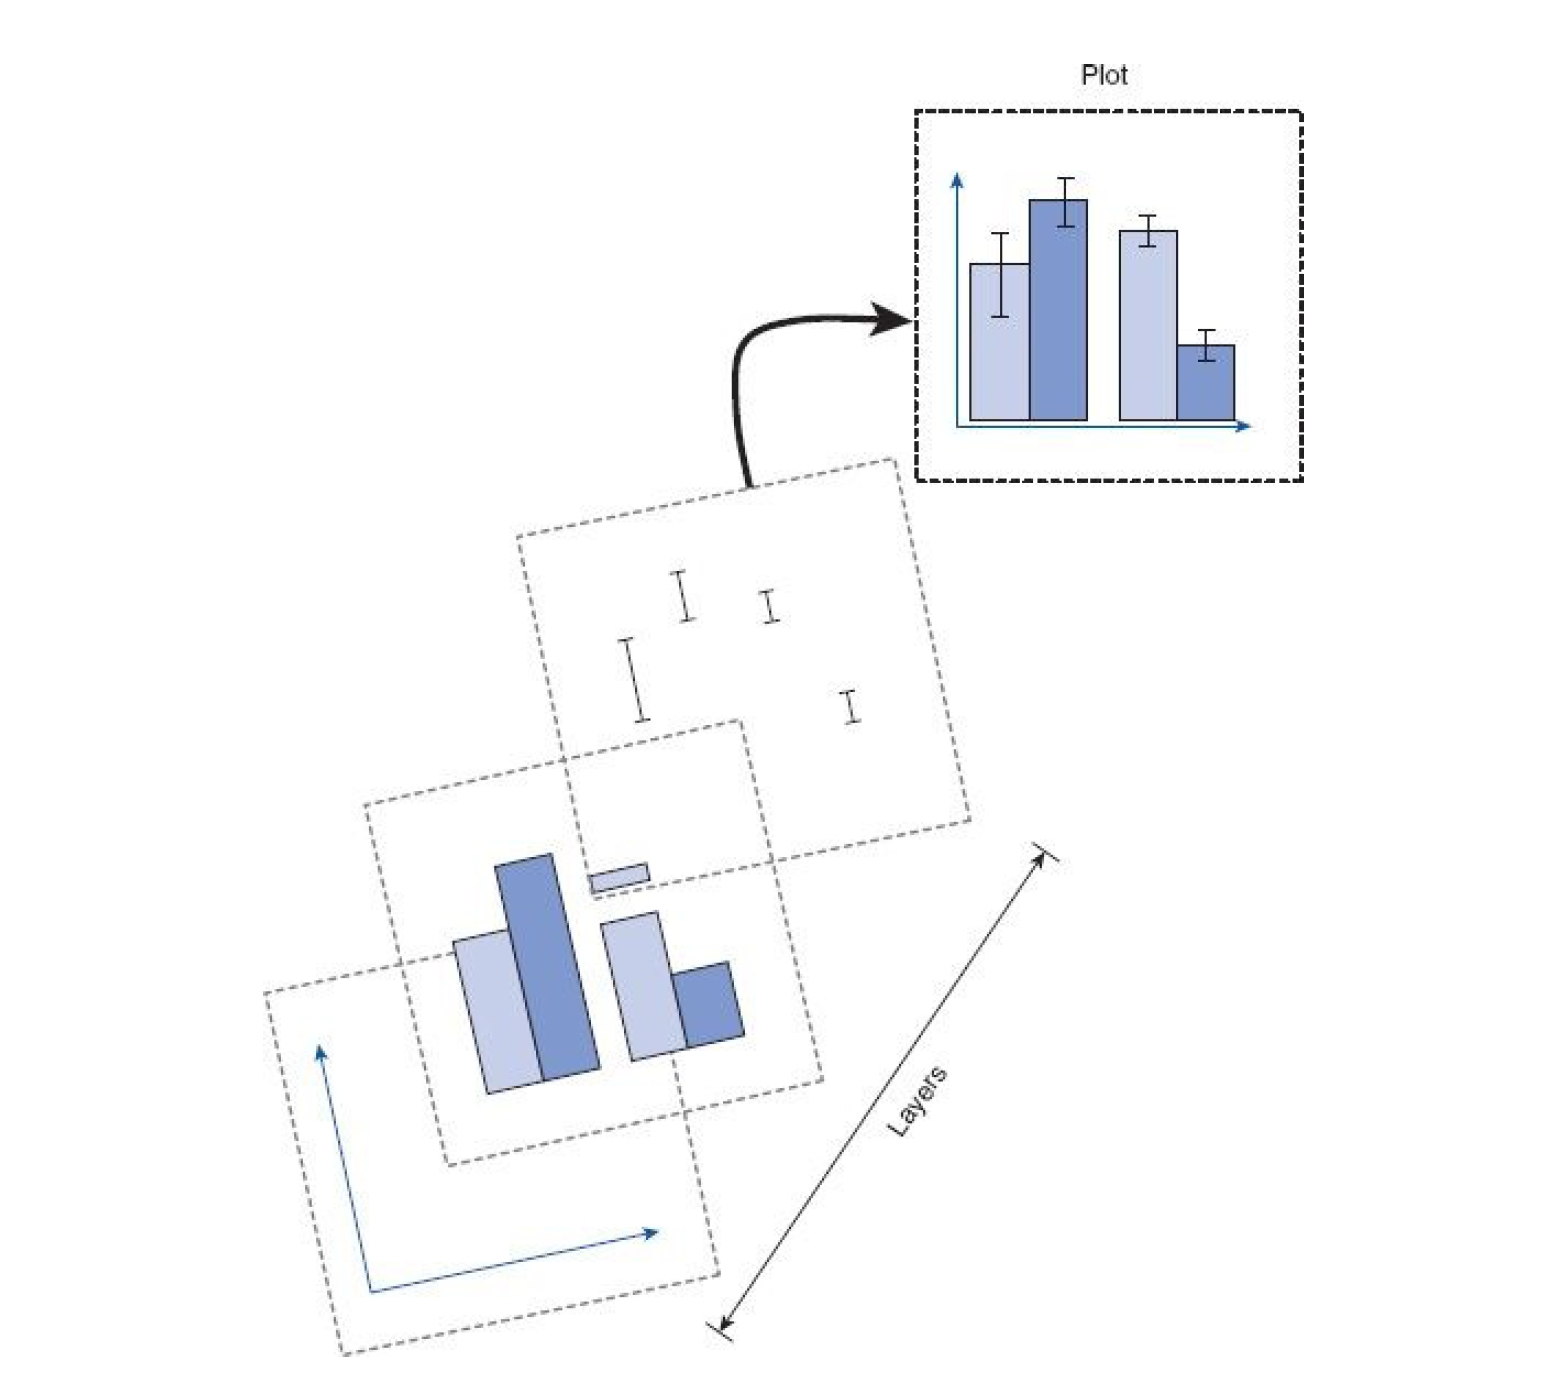
\includegraphics[width=1\linewidth]{images/layers} 

}

\caption{ggplot2 layers from Field et al. (2012)}\label{fig:img-layers}
\end{figure}

\hypertarget{activity-2-set-up}{%
\section{Activity 2: Set-up}\label{activity-2-set-up}}

\begin{itemize}
\tightlist
\item
  Open R Studio and ensure the environment is clear.\\
\item
  Open the \texttt{stub-data-viz.Rmd} file and ensure that the working directory is set to your Data Skills folder and that the two .csv data files (\texttt{participant-info.csv} and \texttt{ahi-cesd.csv}) are in your working directory (you should see them in the file pane).\\
\item
  If you're on the server, avoid a number of issues by restarting the session - click \texttt{Session} - \texttt{Restart\ R}\\
\item
  Type and run the below code to load the \texttt{tidyverse} package and to load in the data files in to the Activity 2 code chunk.
\end{itemize}

\begin{Shaded}
\begin{Highlighting}[]
\FunctionTok{library}\NormalTok{(tidyverse) }

\NormalTok{dat }\OtherTok{\textless{}{-}} \FunctionTok{read\_csv}\NormalTok{(}\StringTok{\textquotesingle{}ahi{-}cesd.csv\textquotesingle{}}\NormalTok{)}
\NormalTok{pinfo }\OtherTok{\textless{}{-}} \FunctionTok{read\_csv}\NormalTok{(}\StringTok{\textquotesingle{}participant{-}info.csv\textquotesingle{}}\NormalTok{)}
\NormalTok{all\_dat }\OtherTok{\textless{}{-}} \FunctionTok{inner\_join}\NormalTok{(dat, pinfo, }\AttributeTok{by=} \FunctionTok{c}\NormalTok{(}\StringTok{"id"}\NormalTok{, }\StringTok{"intervention"}\NormalTok{))}
\NormalTok{summarydata }\OtherTok{\textless{}{-}} \FunctionTok{select}\NormalTok{(}\AttributeTok{.data =}\NormalTok{ all\_dat, }
\NormalTok{                      ahiTotal, cesdTotal, sex, age, }
\NormalTok{                      educ, income, occasion, elapsed.days) }
\end{Highlighting}
\end{Shaded}

\begin{danger}
If you get an error message when using select that says
\texttt{unused\ argument} it means that it is trying to use the wrong
version of the select function. There are two solutions to this, first,
save you work and then restart the R session (click session -restart R)
and then run all your code above again from the start, or replace
\texttt{select} with \texttt{dplyr::select} which tells R exactly which
version of the select function to use. We'd recommend restarting the
session because this will get you in the habit and it's a useful thing
to try for a range of problems
\end{danger}

\hypertarget{activity-3-factors}{%
\section{Activity 3: Factors}\label{activity-3-factors}}

Before we go any further we need to perform an additional step of data processing that we have glossed over up until this point. First, run the below code to look at the structure of the dataset:

\begin{Shaded}
\begin{Highlighting}[]
\FunctionTok{str}\NormalTok{(summarydata)}
\end{Highlighting}
\end{Shaded}

\begin{verbatim}
## tibble [992 x 8] (S3: tbl_df/tbl/data.frame)
##  $ ahiTotal    : num [1:992] 32 34 34 35 36 37 38 38 38 38 ...
##  $ cesdTotal   : num [1:992] 50 49 47 41 36 35 50 55 47 39 ...
##  $ sex         : num [1:992] 1 1 1 1 1 1 2 1 2 2 ...
##  $ age         : num [1:992] 46 37 37 19 40 49 42 57 41 41 ...
##  $ educ        : num [1:992] 4 3 3 2 5 4 4 4 4 4 ...
##  $ income      : num [1:992] 3 2 2 1 2 1 1 2 1 1 ...
##  $ occasion    : num [1:992] 5 2 3 0 5 0 2 2 2 4 ...
##  $ elapsed.days: num [1:992] 182 14.2 33 0 202.1 ...
\end{verbatim}

R assumes that all the variables are numeric (represented by \texttt{num}) and this is going to be a problem because whilst \texttt{sex}, \texttt{educ}, and \texttt{income} are represented by numerical codes, they aren't actually numbers, they're categories, or \textbf{factors}.

We need to tell R that these variables are factors and we can use \texttt{mutate()} to do this by overriding the original variable with the same data but classified as a factor. Type and run the below code to change the categories to factors.

\begin{Shaded}
\begin{Highlighting}[]
\NormalTok{summarydata }\OtherTok{\textless{}{-}}\NormalTok{ summarydata }\SpecialCharTok{\%\textgreater{}\%}
  \FunctionTok{mutate}\NormalTok{(}\AttributeTok{sex =} \FunctionTok{as.factor}\NormalTok{(sex),}
         \AttributeTok{educ =} \FunctionTok{as.factor}\NormalTok{(educ),}
         \AttributeTok{income =} \FunctionTok{as.factor}\NormalTok{(income))}
\end{Highlighting}
\end{Shaded}

You can read this code as ``overwrite the data that is in the column sex with sex as a factor''.

\textbf{Remember this. It's a really important step and if your graphs are looking weird this might be the reason.}

\hypertarget{activity-4-bar-plot}{%
\section{Activity 4: Bar plot}\label{activity-4-bar-plot}}

For our first example we will recreate the bar plot showing the number of male and female participants from Loading Data by showing you how the layers of code build up (next semester we have data that includes non-binary participants).

\begin{itemize}
\tightlist
\item
  The first line (or layer) sets up the base of the graph: the data to use and the aesthetics (what will go on the x and y axis, how the plot will be grouped).\\
\item
  \texttt{aes()} can take both an \texttt{x} and \texttt{y} argument, however, with a bar plot you are just asking R to count the number of data points in each group so you don't need to specify this.
\end{itemize}

\begin{Shaded}
\begin{Highlighting}[]
\FunctionTok{ggplot}\NormalTok{(summarydata, }\FunctionTok{aes}\NormalTok{(}\AttributeTok{x =}\NormalTok{ sex))}
\end{Highlighting}
\end{Shaded}

\begin{figure}

{\centering 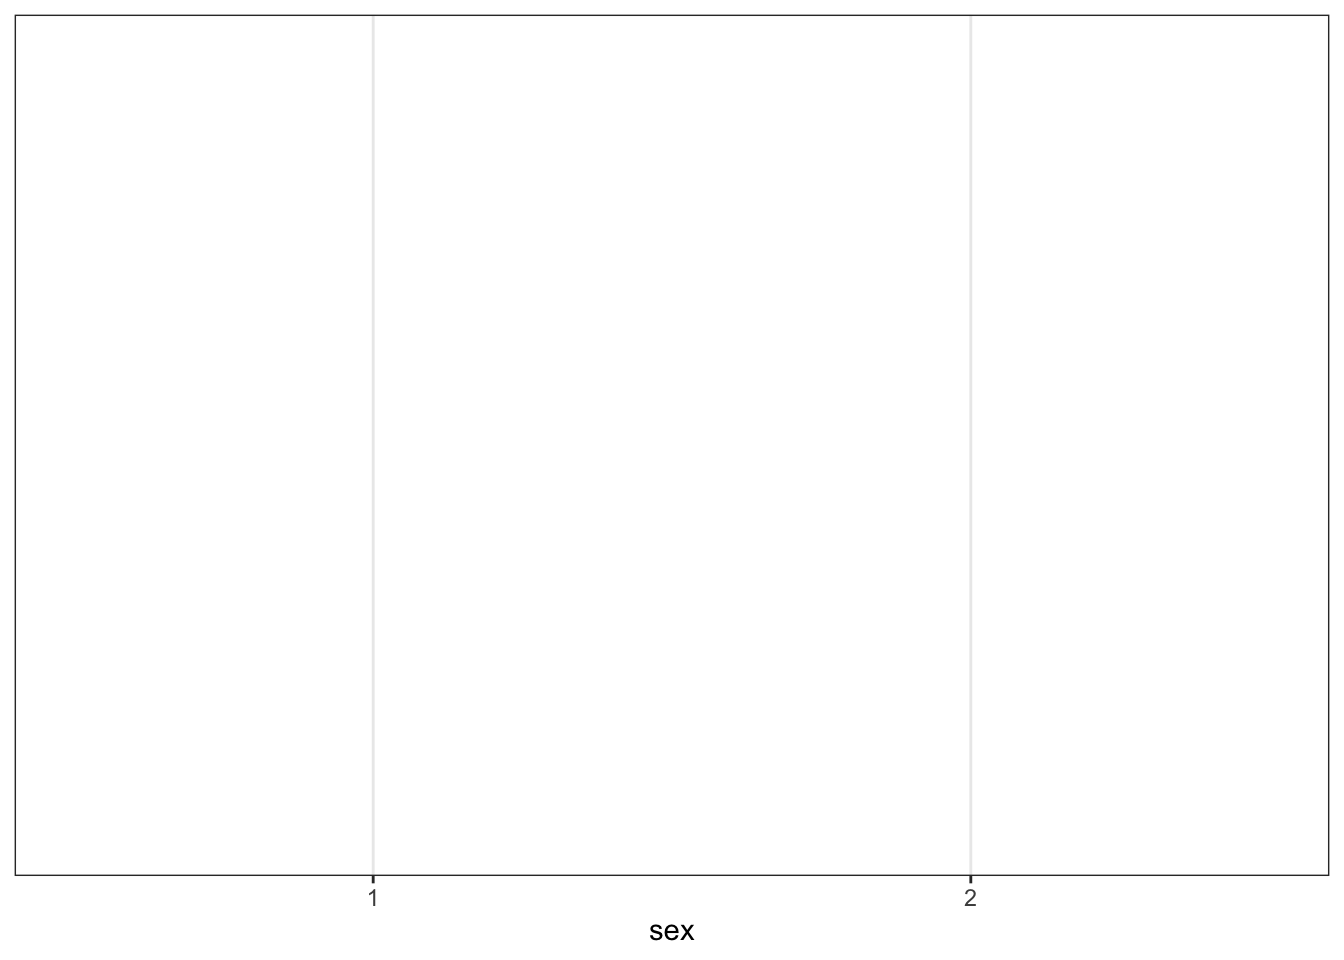
\includegraphics[width=1\linewidth]{07-data-viz_files/figure-latex/layer1-1} 

}

\caption{First ggplot layer sets the axes}\label{fig:layer1}
\end{figure}

\begin{itemize}
\tightlist
\item
  The next layer adds a \textbf{geom} or a shape, in this case we use \texttt{geom\_bar()} as we want to draw a bar plot.
\end{itemize}

\begin{Shaded}
\begin{Highlighting}[]
\FunctionTok{ggplot}\NormalTok{(summarydata, }\FunctionTok{aes}\NormalTok{(}\AttributeTok{x =}\NormalTok{ sex)) }\SpecialCharTok{+}
  \FunctionTok{geom\_bar}\NormalTok{()}
\end{Highlighting}
\end{Shaded}

\begin{figure}

{\centering \includegraphics[width=1\linewidth]{07-data-viz_files/figure-latex/unnamed-chunk-3-1} 

}

\caption{Basic barplot}\label{fig:unnamed-chunk-3}
\end{figure}

\begin{itemize}
\tightlist
\item
  Adding \texttt{fill} to the first layer will separate the data into each level of the grouping variable and give it a different colour. In this case, there is a different coloured bar for each level of \texttt{sex}.
\end{itemize}

\begin{Shaded}
\begin{Highlighting}[]
\FunctionTok{ggplot}\NormalTok{(summarydata, }\FunctionTok{aes}\NormalTok{(}\AttributeTok{x =}\NormalTok{ sex, }\AttributeTok{fill =}\NormalTok{ sex)) }\SpecialCharTok{+}
  \FunctionTok{geom\_bar}\NormalTok{()}
\end{Highlighting}
\end{Shaded}

\begin{figure}

{\centering \includegraphics[width=1\linewidth]{07-data-viz_files/figure-latex/unnamed-chunk-4-1} 

}

\caption{Barplot with colour}\label{fig:unnamed-chunk-4}
\end{figure}

\begin{itemize}
\tightlist
\item
  \texttt{fill()} has also produced a plot legend to the right of the graph. When you have multiple grouping variables you need this to know which groups each bit of the plot is referring to, but in this case it is redundant because it doesn't tell us anything that the axis labels don't already. We can get rid of it by adding \texttt{show.legend\ =\ FALSE} to the \texttt{geom\_bar()} code.
\end{itemize}

\begin{Shaded}
\begin{Highlighting}[]
\FunctionTok{ggplot}\NormalTok{(summarydata, }\FunctionTok{aes}\NormalTok{(}\AttributeTok{x =}\NormalTok{ sex, }\AttributeTok{fill =}\NormalTok{ sex)) }\SpecialCharTok{+}
  \FunctionTok{geom\_bar}\NormalTok{(}\AttributeTok{show.legend =} \ConstantTok{FALSE}\NormalTok{)}
\end{Highlighting}
\end{Shaded}

\begin{figure}

{\centering \includegraphics[width=1\linewidth]{07-data-viz_files/figure-latex/unnamed-chunk-5-1} 

}

\caption{Barplot without legend}\label{fig:unnamed-chunk-5}
\end{figure}

We might want to tidy up our plot to make it look a bit nicer. First we can edit the axis labels to be more informative. The most common functions you will use are:

\begin{itemize}
\tightlist
\item
  \texttt{scale\_x\_continuous()} for adjusting the x-axis for a continuous variable
\item
  \texttt{scale\_y\_continuous()} for adjusting the y-axis for a continuous variable
\item
  \texttt{scale\_x\_discrete()} for adjusting the x-axis for a discrete/categorical variable
\item
  \texttt{scale\_y\_discrete()} for adjusting the y-axis for a discrete/categorical variable
\end{itemize}

And in those functions the two most common arguments you will use are:

\begin{itemize}
\tightlist
\item
  \texttt{name} which controls the name of each axis
\item
  \texttt{labels} which controls the names of the break points on the axis
\end{itemize}

There are lots more ways you can customise your axes but we'll stick with these for now. Copy, paste, and run the below code to change the axis labels and change the numeric sex codes into words.

\begin{Shaded}
\begin{Highlighting}[]
\FunctionTok{ggplot}\NormalTok{(summarydata, }\FunctionTok{aes}\NormalTok{(}\AttributeTok{x =}\NormalTok{ sex, }\AttributeTok{fill =}\NormalTok{ sex)) }\SpecialCharTok{+}
  \FunctionTok{geom\_bar}\NormalTok{(}\AttributeTok{show.legend =} \ConstantTok{FALSE}\NormalTok{) }\SpecialCharTok{+}
  \FunctionTok{scale\_x\_discrete}\NormalTok{(}\AttributeTok{name =} \StringTok{"Participant Sex"}\NormalTok{, }
                   \AttributeTok{labels =} \FunctionTok{c}\NormalTok{(}\StringTok{"Female"}\NormalTok{, }\StringTok{"Male"}\NormalTok{)) }\SpecialCharTok{+}
  \FunctionTok{scale\_y\_continuous}\NormalTok{(}\AttributeTok{name =} \StringTok{"Number of participants"}\NormalTok{)}
\end{Highlighting}
\end{Shaded}

\begin{figure}

{\centering 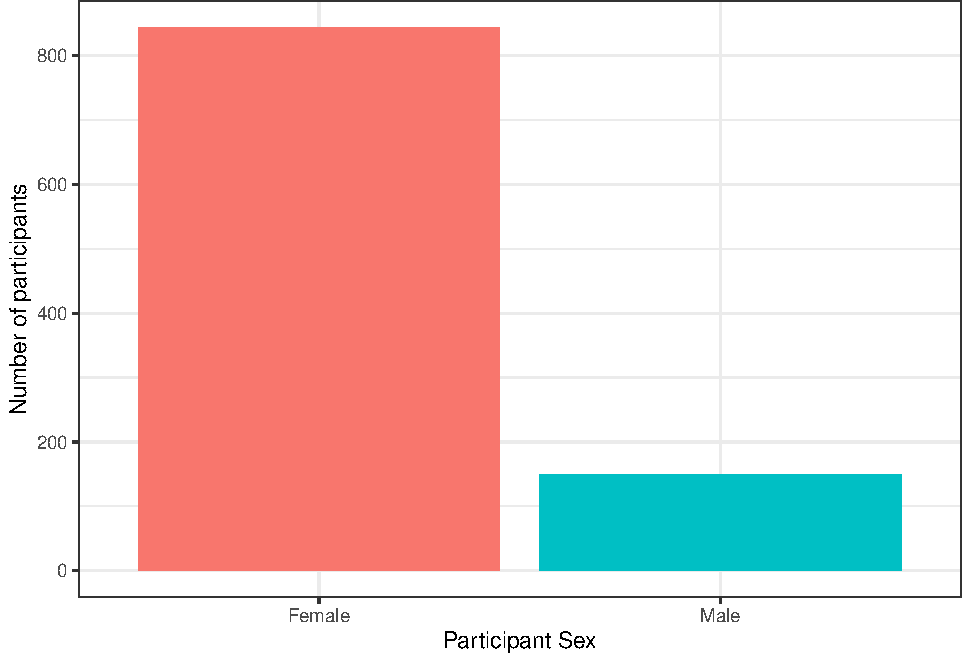
\includegraphics[width=1\linewidth]{07-data-viz_files/figure-latex/unnamed-chunk-6-1} 

}

\caption{Barplot with axis labels}\label{fig:unnamed-chunk-6}
\end{figure}

Second, you might want to adjust the colours and the visual style of the plot. \texttt{ggplot2} comes with built in themes. Below, we'll use \texttt{theme\_minimal()} but try typing \texttt{theme\_} into a code chunk and try all the options that come up to see which one you like best.

\begin{Shaded}
\begin{Highlighting}[]
\FunctionTok{ggplot}\NormalTok{(summarydata, }\FunctionTok{aes}\NormalTok{(}\AttributeTok{x =}\NormalTok{ sex, }\AttributeTok{fill =}\NormalTok{ sex)) }\SpecialCharTok{+}
  \FunctionTok{geom\_bar}\NormalTok{(}\AttributeTok{show.legend =} \ConstantTok{FALSE}\NormalTok{) }\SpecialCharTok{+}
  \FunctionTok{scale\_x\_discrete}\NormalTok{(}\AttributeTok{name =} \StringTok{"Participant Sex"}\NormalTok{, }
                   \AttributeTok{labels =} \FunctionTok{c}\NormalTok{(}\StringTok{"Female"}\NormalTok{, }\StringTok{"Male"}\NormalTok{)) }\SpecialCharTok{+}
  \FunctionTok{scale\_y\_continuous}\NormalTok{(}\AttributeTok{name =} \StringTok{"Number of participants"}\NormalTok{) }\SpecialCharTok{+}
  \FunctionTok{theme\_minimal}\NormalTok{()}
\end{Highlighting}
\end{Shaded}

\begin{figure}

{\centering 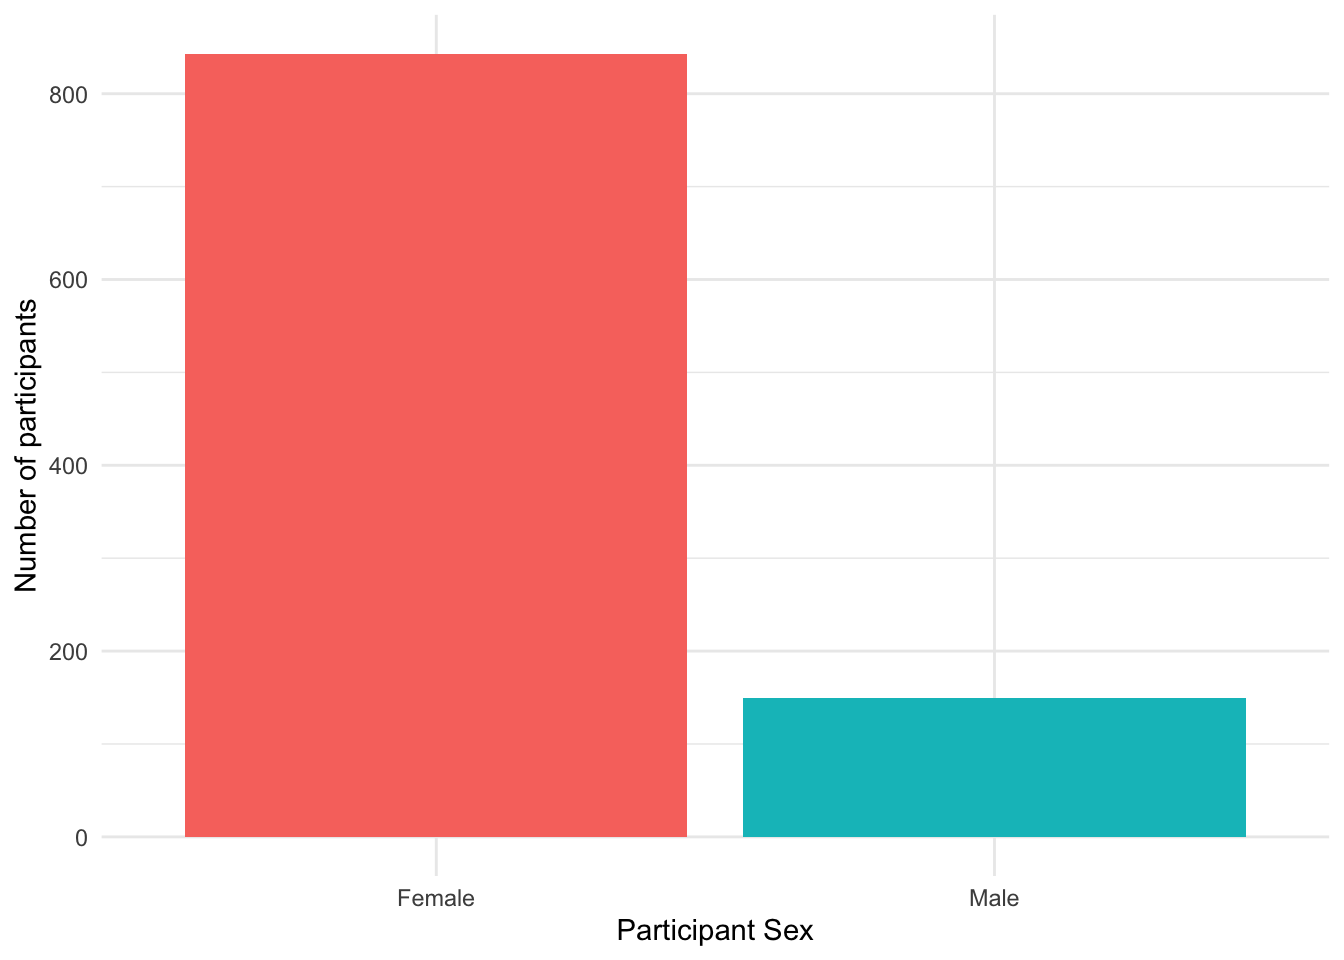
\includegraphics[width=1\linewidth]{07-data-viz_files/figure-latex/unnamed-chunk-7-1} 

}

\caption{Barplot with minimal theme}\label{fig:unnamed-chunk-7}
\end{figure}

There are various options to adjust the colours but a good way to be inclusive is to use a colour-blind friendly palette that can also be read if printed in black-and-white. To do this, we can add on the function \texttt{scale\_fill\_viridis\_d()}. This function has 5 colour options, A, B, C, D, and E. I prefer E but you can play around with them and choose the one you prefer.

\begin{Shaded}
\begin{Highlighting}[]
\FunctionTok{ggplot}\NormalTok{(summarydata, }\FunctionTok{aes}\NormalTok{(}\AttributeTok{x =}\NormalTok{ sex, }\AttributeTok{fill =}\NormalTok{ sex)) }\SpecialCharTok{+}
  \FunctionTok{geom\_bar}\NormalTok{(}\AttributeTok{show.legend =} \ConstantTok{FALSE}\NormalTok{) }\SpecialCharTok{+}
  \FunctionTok{scale\_x\_discrete}\NormalTok{(}\AttributeTok{name =} \StringTok{"Participant Sex"}\NormalTok{, }
                   \AttributeTok{labels =} \FunctionTok{c}\NormalTok{(}\StringTok{"Female"}\NormalTok{, }\StringTok{"Male"}\NormalTok{)) }\SpecialCharTok{+}
  \FunctionTok{scale\_y\_continuous}\NormalTok{(}\AttributeTok{name =} \StringTok{"Number of participants"}\NormalTok{) }\SpecialCharTok{+}
  \FunctionTok{theme\_minimal}\NormalTok{() }\SpecialCharTok{+}
  \FunctionTok{scale\_fill\_viridis\_d}\NormalTok{(}\AttributeTok{option =} \StringTok{"E"}\NormalTok{)}
\end{Highlighting}
\end{Shaded}

\begin{figure}

{\centering \includegraphics[width=1\linewidth]{07-data-viz_files/figure-latex/unnamed-chunk-8-1} 

}

\caption{Barplot with colour-blind friendly colour scheme}\label{fig:unnamed-chunk-8}
\end{figure}

Finally, you can also adjust the transparency of the bars by adding \texttt{alpha} to \texttt{geom\_bar()}. Play around with the value and see what value you prefer.

\begin{Shaded}
\begin{Highlighting}[]
\FunctionTok{ggplot}\NormalTok{(summarydata, }\FunctionTok{aes}\NormalTok{(}\AttributeTok{x =}\NormalTok{ sex, }\AttributeTok{fill =}\NormalTok{ sex)) }\SpecialCharTok{+}
  \FunctionTok{geom\_bar}\NormalTok{(}\AttributeTok{show.legend =} \ConstantTok{FALSE}\NormalTok{, }\AttributeTok{alpha =}\NormalTok{ .}\DecValTok{8}\NormalTok{) }\SpecialCharTok{+}
  \FunctionTok{scale\_x\_discrete}\NormalTok{(}\AttributeTok{name =} \StringTok{"Participant Sex"}\NormalTok{, }
                   \AttributeTok{labels =} \FunctionTok{c}\NormalTok{(}\StringTok{"Female"}\NormalTok{, }\StringTok{"Male"}\NormalTok{)) }\SpecialCharTok{+}
  \FunctionTok{scale\_y\_continuous}\NormalTok{(}\AttributeTok{name =} \StringTok{"Number of participants"}\NormalTok{) }\SpecialCharTok{+}
  \FunctionTok{theme\_minimal}\NormalTok{() }\SpecialCharTok{+}
  \FunctionTok{scale\_fill\_viridis\_d}\NormalTok{(}\AttributeTok{option =} \StringTok{"E"}\NormalTok{)}
\end{Highlighting}
\end{Shaded}

\begin{figure}

{\centering \includegraphics[width=1\linewidth]{07-data-viz_files/figure-latex/unnamed-chunk-9-1} 

}

\caption{Barplot with adjusted alpha}\label{fig:unnamed-chunk-9}
\end{figure}

\begin{warning}
In R terms, \texttt{ggplot2} is a fairly old package. As a result, the
use of pipes wasn't included when it was originally written. As you can
see in the code above, the layers of the code are separated by
\texttt{+} rather than \texttt{\%\textgreater{}\%}. In this case,
\texttt{+} is doing essentially the same job as a pipe - be careful not
to confuse them.
\end{warning}

\hypertarget{activity-5-violin-boxplot}{%
\section{Activity 5: Violin-boxplot}\label{activity-5-violin-boxplot}}

As our final activity we will also explain the code used to create the violin-boxplot from Loading Data, hopefully now you will be able to see how similar it is in structure to the bar chart code. In fact, there are only three differences:

\begin{enumerate}
\def\labelenumi{\arabic{enumi}.}
\tightlist
\item
  We have added a \texttt{y} argument to the first layer because we wanted to represent two variables, not just a count.
\item
  \texttt{geom\_violin()} has an additional argument \texttt{trim}. Try setting this to \texttt{TRUE} to see what happens.
\item
  \texttt{geom\_boxpot()} has an additional argument \texttt{width}. Try adjusting the value of this and see what happens.
\end{enumerate}

\begin{Shaded}
\begin{Highlighting}[]
\FunctionTok{ggplot}\NormalTok{(summarydata, }\FunctionTok{aes}\NormalTok{(}\AttributeTok{x =}\NormalTok{ income, }\AttributeTok{y =}\NormalTok{ ahiTotal, }\AttributeTok{fill =}\NormalTok{ income)) }\SpecialCharTok{+}
  \FunctionTok{geom\_violin}\NormalTok{(}\AttributeTok{trim =} \ConstantTok{FALSE}\NormalTok{, }\AttributeTok{show.legend =} \ConstantTok{FALSE}\NormalTok{, }\AttributeTok{alpha =}\NormalTok{ .}\DecValTok{4}\NormalTok{) }\SpecialCharTok{+}
  \FunctionTok{geom\_boxplot}\NormalTok{(}\AttributeTok{width =}\NormalTok{ .}\DecValTok{2}\NormalTok{, }\AttributeTok{show.legend =} \ConstantTok{FALSE}\NormalTok{, }\AttributeTok{alpha =}\NormalTok{ .}\DecValTok{7}\NormalTok{)}\SpecialCharTok{+}
  \FunctionTok{scale\_x\_discrete}\NormalTok{(}\AttributeTok{name =} \StringTok{"Income"}\NormalTok{,}
                   \AttributeTok{labels =} \FunctionTok{c}\NormalTok{(}\StringTok{"Below Average"}\NormalTok{, }\StringTok{"Average"}\NormalTok{, }\StringTok{"Above Average"}\NormalTok{)) }\SpecialCharTok{+}
  \FunctionTok{scale\_y\_continuous}\NormalTok{(}\AttributeTok{name =} \StringTok{"Authentic Happiness Inventory Score"}\NormalTok{)}\SpecialCharTok{+}
  \FunctionTok{theme\_minimal}\NormalTok{() }\SpecialCharTok{+}
  \FunctionTok{scale\_fill\_viridis\_d}\NormalTok{()}
\end{Highlighting}
\end{Shaded}

\begin{figure}

{\centering \includegraphics[width=1\linewidth]{07-data-viz_files/figure-latex/unnamed-chunk-11-1} 

}

\caption{Violin-boxplot}\label{fig:unnamed-chunk-11}
\end{figure}

\hypertarget{activity-6-layers-part-2}{%
\section{Activity 6: Layers part 2}\label{activity-6-layers-part-2}}

The key thing to note about \texttt{ggplot} is the use of layers. Whilst we've built this up step-by-step, they are independent and you could remove any of them except for the first layer. Additionally, although they are independent, the order you put them in does matter. Try running the two code examples below and see what happens.

\begin{Shaded}
\begin{Highlighting}[]
\FunctionTok{ggplot}\NormalTok{(summarydata, }\FunctionTok{aes}\NormalTok{(}\AttributeTok{x =}\NormalTok{ income, }\AttributeTok{y =}\NormalTok{ ahiTotal)) }\SpecialCharTok{+}
  \FunctionTok{geom\_violin}\NormalTok{() }\SpecialCharTok{+}
  \FunctionTok{geom\_boxplot}\NormalTok{()}

\FunctionTok{ggplot}\NormalTok{(summarydata, }\FunctionTok{aes}\NormalTok{(}\AttributeTok{x =}\NormalTok{ income, }\AttributeTok{y =}\NormalTok{ ahiTotal)) }\SpecialCharTok{+}
  \FunctionTok{geom\_boxplot}\NormalTok{() }\SpecialCharTok{+}
  \FunctionTok{geom\_violin}\NormalTok{()}
\end{Highlighting}
\end{Shaded}

\hypertarget{finished-4}{%
\subsubsection{Finished!}\label{finished-4}}

Well done! \texttt{ggplot} can be a bit difficult to get your head around at first, particularly if you've been used to making graphs a different way. But once it clicks, you'll be able to make informative and professional visualisations with ease, which, amongst other things, will make your reports look FANCY.

\hypertarget{scatterplots}{%
\chapter{Scatterplots}\label{scatterplots}}

In this chapter we will work with our data to generate a plot of two variables from the Woodworth et al.~dataset. Before we get to generate our plot, we still need to work through the steps to get the data in the shape we need it to be in for our particular question. In particular we need to generate the object \texttt{summarydata} that just has the variable we need.You have done these steps before so go back to the relevant Lab and use that to guide you through.

\hypertarget{activity-1-set-up-3}{%
\section{Activity 1: Set-up}\label{activity-1-set-up-3}}

\begin{itemize}
\tightlist
\item
  Open R Studio and ensure the environment is clear.\\
\item
  Open the \texttt{stub-scatterplot.Rmd} file and ensure that the working directory is set to your Data Skills folder and that the two .csv data files (\texttt{participant-info.csv} and \texttt{ahi-cesd.csv}) are in your working directory (you should see them in the file pane).\\
\item
  Look through your previous work to find the code that loads the \texttt{tidyverse}, reads in the data files and creates an object called \texttt{all\_dat} that joins the two objects \texttt{dat} and \texttt{pinfo}.
\end{itemize}

\hypertarget{activity-2-select-1}{%
\section{Activity 2: Select}\label{activity-2-select-1}}

Select the columns \texttt{ahiTotal}, \texttt{cesdTotal}, \texttt{sex}, \texttt{age}, \texttt{educ} from the \texttt{all\_dat} and save them in a new object named variable \texttt{summarydata}.

\hypertarget{activity-3-simple-scatterplots}{%
\section{Activity 3: Simple scatterplots}\label{activity-3-simple-scatterplots}}

First, we want to look at whether there seems to be a relationship between happiness and depression scores across all participants.

In order to visualise two continuous variables, we can use a \textbf{scatterplot}. Using the \texttt{ggplot} code you learned about in Intro to Data Viz, try and recreate the below plot.

A few hints:

\begin{itemize}
\tightlist
\item
  Use the \texttt{summarydata} data.
\item
  Put \texttt{ahiTotal} on the x-axis and \texttt{cesdTotal} on the y-axis.
\item
  Rather than using \texttt{geom\_bar()}, \texttt{geom\_violin()}, or \texttt{geom\_boxplot()}, for a scatterplot you need to use \texttt{geom\_point()}.
\item
  Rather than using \texttt{scale\_fill\_viridis\_d()} to change the colour, add the argument \texttt{colour\ =\ "red"} to \texttt{geom\_point} (except replace ``red'' with whatever colour you'd prefer).
\item
  Remember to edit the axis names.
\end{itemize}

\begin{figure}

{\centering 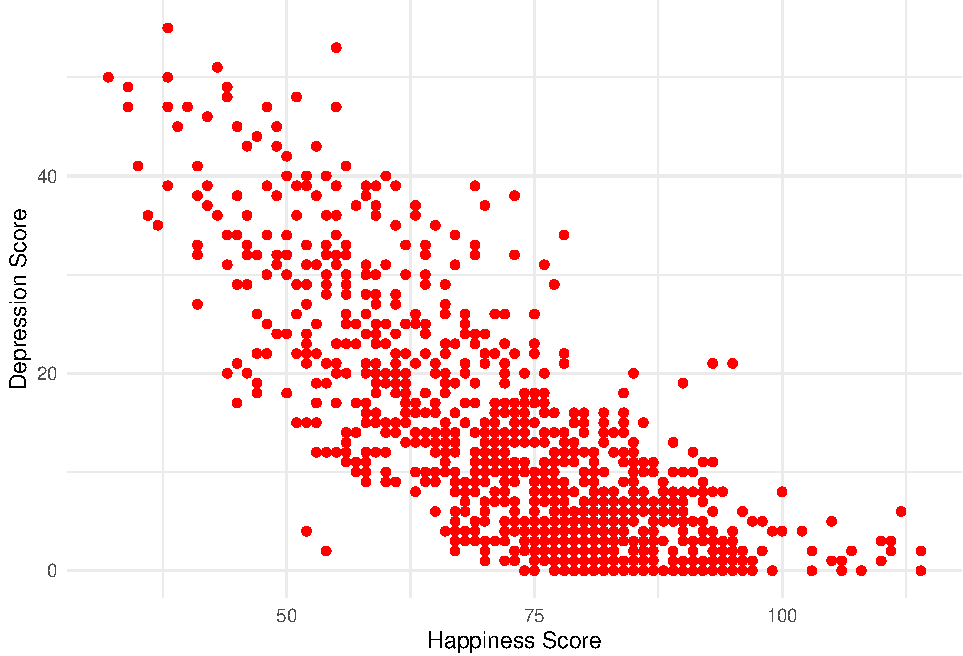
\includegraphics[width=1\linewidth]{08-scatterplots_files/figure-latex/createplot-1} 

}

\caption{Scatterplot of happiness and depression scores}\label{fig:createplot}
\end{figure}

How would you describe the relationship between the two variables? As happiness scores increase, depression scores increaseAs happiness score increase, depression scores decreaseAs happiness scores decrease, depression scores decrease

\hypertarget{activity-4-adding-a-line-of-best-fit}{%
\section{Activity 4: Adding a line of best fit}\label{activity-4-adding-a-line-of-best-fit}}

Scatterplots are very useful but it can often help to add a line of best fit to help interpretation. Add the below layer to the scatterplot code from Activity 4:

\begin{itemize}
\tightlist
\item
  This code uses the function \texttt{geom\_smooth()} to draw the line. There are several different methods but we want a straight, or linear, line so we specify \texttt{method\ =\ "lm"}.
\item
  This line is really a regression line, which you'll learn more about in level 2. For now, the steeper the slope of the line, the stronger the relationship between the two variables.
\item
  By default the regression line will be extended, beyond the original y-axis limits, if you want to change this so that your plots looks like the below, add \texttt{limits\ =\ c(0,60)} to \texttt{scale\_y\_continuous()}
\end{itemize}

\begin{Shaded}
\begin{Highlighting}[]
\FunctionTok{geom\_smooth}\NormalTok{(}\AttributeTok{method =} \StringTok{"lm"}\NormalTok{)}
\end{Highlighting}
\end{Shaded}

\begin{figure}

{\centering 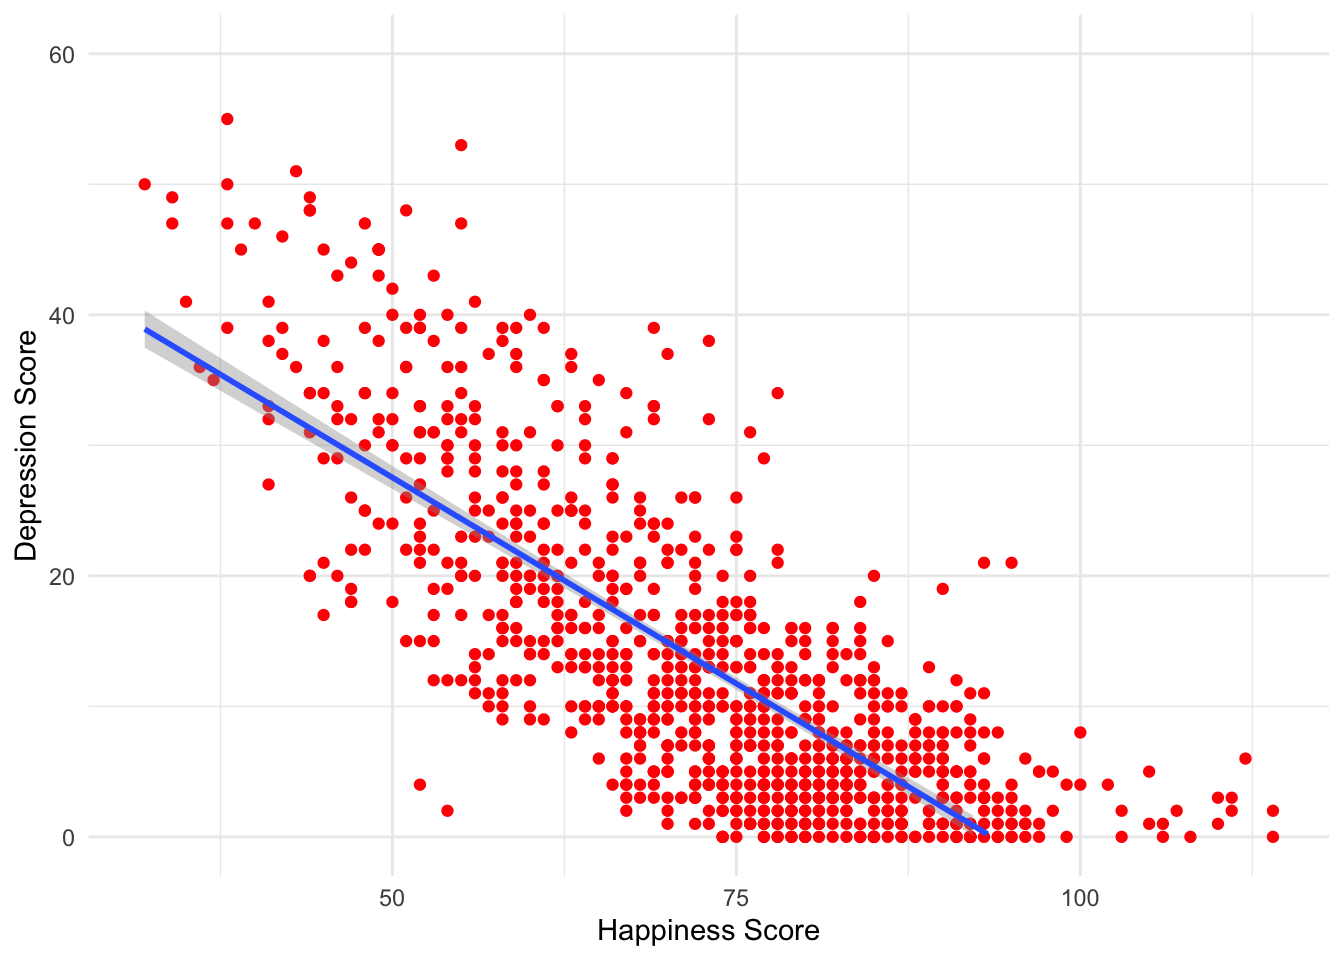
\includegraphics[width=1\linewidth]{08-scatterplots_files/figure-latex/createplot2-1} 

}

\caption{Scatterplot of happiness and depression scores}\label{fig:createplot2}
\end{figure}

\hypertarget{activity-5-setting-the-factors}{%
\section{Activity 5: Setting the factors}\label{activity-5-setting-the-factors}}

It seems fairly obvious that there might be a negative relationship between happiness and depression, so instead we want to look at whether this relationship changes depending on different demographic variables.

Just like in the last chapter, we need to ensure that R knows what type of data each variable is. At the moment, \texttt{sex}, \texttt{educ}, and \texttt{income} are all registered as numeric variables, but we know that they're really categories.

\begin{Shaded}
\begin{Highlighting}[]
\FunctionTok{str}\NormalTok{(summarydata)}
\end{Highlighting}
\end{Shaded}

\begin{verbatim}
## tibble [992 x 6] (S3: tbl_df/tbl/data.frame)
##  $ ahiTotal : num [1:992] 32 34 34 35 36 37 38 38 38 38 ...
##  $ cesdTotal: num [1:992] 50 49 47 41 36 35 50 55 47 39 ...
##  $ sex      : num [1:992] 1 1 1 1 1 1 2 1 2 2 ...
##  $ age      : num [1:992] 46 37 37 19 40 49 42 57 41 41 ...
##  $ educ     : num [1:992] 4 3 3 2 5 4 4 4 4 4 ...
##  $ income   : num [1:992] 3 2 2 1 2 1 1 2 1 1 ...
\end{verbatim}

\begin{itemize}
\tightlist
\item
  Using the same method you used in the last chapter, overwrite \texttt{sex}, \texttt{educ} and \texttt{income} in \texttt{summarydata} as factors.
\end{itemize}

\hypertarget{activity-6-grouped-scatterplots}{%
\section{Activity 6: Grouped scatterplots}\label{activity-6-grouped-scatterplots}}

We can now use our factors to display the data in the scatterplots for each group.

\begin{itemize}
\tightlist
\item
  Rather than adding \texttt{colour} to \texttt{geom\_point()} which sets the colour for all the data points, instead we add \texttt{colour\ =\ sex} to the aesthetic mapping on the first line. This tells \texttt{ggplot()} to produce different colours for each level (or group) in the variable \texttt{sex}.
\item
  \texttt{scale\_color\_viridis\_d()} works exactly like the other colour blind friendly scale functions you have used, so we can use \texttt{name} and \texttt{labels} to adjust the legend.
\end{itemize}

\begin{Shaded}
\begin{Highlighting}[]
\FunctionTok{ggplot}\NormalTok{(summarydata, }\FunctionTok{aes}\NormalTok{(}\AttributeTok{x =}\NormalTok{ ahiTotal , }\AttributeTok{y =}\NormalTok{ cesdTotal, }\AttributeTok{colour =}\NormalTok{ sex)) }\SpecialCharTok{+} 
  \FunctionTok{geom\_point}\NormalTok{() }\SpecialCharTok{+}
  \FunctionTok{scale\_x\_continuous}\NormalTok{(}\AttributeTok{name =} \StringTok{"Happiness Score"}\NormalTok{) }\SpecialCharTok{+}
  \FunctionTok{scale\_y\_continuous}\NormalTok{(}\AttributeTok{name =} \StringTok{"Depression Score"}\NormalTok{,}
                     \AttributeTok{limits =} \FunctionTok{c}\NormalTok{(}\DecValTok{0}\NormalTok{,}\DecValTok{60}\NormalTok{)) }\SpecialCharTok{+}
  \FunctionTok{theme\_minimal}\NormalTok{() }\SpecialCharTok{+}
  \FunctionTok{geom\_smooth}\NormalTok{(}\AttributeTok{method =} \StringTok{"lm"}\NormalTok{, }\AttributeTok{formula =}\NormalTok{ y}\SpecialCharTok{\textasciitilde{}}\NormalTok{x) }\SpecialCharTok{+}
  \FunctionTok{scale\_color\_viridis\_d}\NormalTok{(}\AttributeTok{name =} \StringTok{"Participant sex"}\NormalTok{, }
                       \AttributeTok{labels =} \FunctionTok{c}\NormalTok{(}\StringTok{"Male"}\NormalTok{, }\StringTok{"Female"}\NormalTok{),}
                       \AttributeTok{option =} \StringTok{"E"}\NormalTok{)}
\end{Highlighting}
\end{Shaded}

\begin{center}\includegraphics[width=1\linewidth]{08-scatterplots_files/figure-latex/unnamed-chunk-4-1} \end{center}

It looks like the relationship between happiness and depression is about the same for male and female participants.

\begin{itemize}
\tightlist
\item
  Create two more scatterplots that show the relationship between happiness and depression grouped by a) \texttt{income} and b) \texttt{educ}. Make sure you update the legend labels (you might need to check the code book).
\end{itemize}

\hypertarget{activity-7-group-by-a-new-variable}{%
\section{Activity 7: Group by a new variable}\label{activity-7-group-by-a-new-variable}}

So, let's be honest, there's not much going on with any of the demographic variables - the relationship between depression and anxiety is pretty much the same for all of the groups. A reasonable hypothesis might be that rather than being connected to any demographic variables, the relationship between happiness and depression changes depending upon your general happiness level.

\begin{itemize}
\tightlist
\item
  Using \texttt{mutate} create a new variable named \texttt{happiness} in \texttt{summarydata} that evaluates whether a participant's happiness score is equal to or higher than the median \texttt{ahiTotal} score.
\item
  This is not an easy task as it's not something we've explicitly shown you how to do but it's the last activity for this semester so before you go to the solution, do a bit of trial and error, then look at the hints to see if you can get near the answer.
\item
  If you've done it right, \texttt{summarydata} should contain a column named \texttt{happiness} with the value \texttt{TRUE} if \texttt{ahiTotal} is above the overall median and \texttt{FALSE} if it is below.
\end{itemize}

Hint 1

\begin{Shaded}
\begin{Highlighting}[]
\FunctionTok{mutate}\NormalTok{(data, }\AttributeTok{new\_variable =}\NormalTok{ equal\_or\_more\_than\_median)}
\end{Highlighting}
\end{Shaded}

Hint 2

\begin{Shaded}
\begin{Highlighting}[]
\FunctionTok{mutate}\NormalTok{(data, }\AttributeTok{new\_variable =}\NormalTok{ variable }\SpecialCharTok{\textgreater{}=} \FunctionTok{median}\NormalTok{(variable))}
\end{Highlighting}
\end{Shaded}

Now, reproduce the below plot using this new variable:

\begin{center}\includegraphics[width=1\linewidth]{08-scatterplots_files/figure-latex/unnamed-chunk-8-1} \end{center}

What might you conclude from this plot? The relationship between happiness and depression scores is stronger for people who have above average happiness scoresThe relationsip between happiness and depression scores is stronger for people who have lower than average happiness scoresThere is no difference in the relationship between depression and happiness scores between the groups

Explain this answer

The line for the ``unhappy'' group is much steeper than the line for the ``happy'' group. That is, is you're generally unhappy, then you report a much stronger link between your happiness and depression levels than if you're generally happy.

If you actually wanted to look at the difference in the relationships statistically, you could compute the correlation coefficients like below, but don't worry about that until Level 2.

\begin{Shaded}
\begin{Highlighting}[]
\NormalTok{dat\_above }\OtherTok{\textless{}{-}} \FunctionTok{filter}\NormalTok{(summarydata, happiness }\SpecialCharTok{==} \ConstantTok{TRUE}\NormalTok{)}
\NormalTok{dat\_below }\OtherTok{\textless{}{-}} \FunctionTok{filter}\NormalTok{(summarydata, happiness }\SpecialCharTok{==} \ConstantTok{FALSE}\NormalTok{)}

\FunctionTok{cor.test}\NormalTok{(dat\_above}\SpecialCharTok{$}\NormalTok{ahiTotal, dat\_above}\SpecialCharTok{$}\NormalTok{cesdTotal)}
\FunctionTok{cor.test}\NormalTok{(dat\_below}\SpecialCharTok{$}\NormalTok{ahiTotal, dat\_below}\SpecialCharTok{$}\NormalTok{cesdTotal)}
\end{Highlighting}
\end{Shaded}

\begin{verbatim}
## 
##  Pearson's product-moment correlation
## 
## data:  dat_above$ahiTotal and dat_above$cesdTotal
## t = -7.6564, df = 491, p-value = 1.024e-13
## alternative hypothesis: true correlation is not equal to 0
## 95 percent confidence interval:
##  -0.4032637 -0.2453473
## sample estimates:
##        cor 
## -0.3265828 
## 
## 
##  Pearson's product-moment correlation
## 
## data:  dat_below$ahiTotal and dat_below$cesdTotal
## t = -22.474, df = 497, p-value < 2.2e-16
## alternative hypothesis: true correlation is not equal to 0
## 95 percent confidence interval:
##  -0.7509362 -0.6635268
## sample estimates:
##        cor 
## -0.7099551
\end{verbatim}

\hypertarget{finished-5}{%
\subsection{Finished!}\label{finished-5}}

Great job! As you may have noticed, this chapter tried to push you and test what you've learned - we hope you can see just how far you've come in the space of just a couple of months, it's genuinely amazing what you have achieved and you should feel proud. In Psych 1B we will continue using these wrangling skills on new data and also data that you collect yourself.

\hypertarget{activity-solutions---scatterplots}{%
\section{Activity solutions - Scatterplots}\label{activity-solutions---scatterplots}}

\hypertarget{activity-1-2}{%
\subsection{Activity 1}\label{activity-1-2}}

Solution

\begin{Shaded}
\begin{Highlighting}[]
\FunctionTok{library}\NormalTok{(tidyverse)}
\NormalTok{dat }\OtherTok{\textless{}{-}} \FunctionTok{read\_csv}\NormalTok{ (}\StringTok{\textquotesingle{}ahi{-}cesd.csv\textquotesingle{}}\NormalTok{)}
\NormalTok{pinfo }\OtherTok{\textless{}{-}} \FunctionTok{read\_csv}\NormalTok{(}\StringTok{\textquotesingle{}participant{-}info.csv\textquotesingle{}}\NormalTok{)}
\NormalTok{all\_dat }\OtherTok{\textless{}{-}} \FunctionTok{inner\_join}\NormalTok{(dat, pinfo, }\AttributeTok{by=}\FunctionTok{c}\NormalTok{(}\StringTok{"id"}\NormalTok{, }\StringTok{"intervention"}\NormalTok{)}
\end{Highlighting}
\end{Shaded}

\hypertarget{activity-2-2}{%
\subsection{Activity 2}\label{activity-2-2}}

Solution

\begin{Shaded}
\begin{Highlighting}[]
\NormalTok{summarydata }\OtherTok{\textless{}{-}} \FunctionTok{select}\NormalTok{(all\_dat, ahiTotal, cesdTotal, sex, age, educ, income)}
\end{Highlighting}
\end{Shaded}

\hypertarget{activity-3-1}{%
\subsection{Activity 3}\label{activity-3-1}}

Solution

\begin{Shaded}
\begin{Highlighting}[]
\FunctionTok{ggplot}\NormalTok{(all\_dat, }\FunctionTok{aes}\NormalTok{(}\AttributeTok{x =}\NormalTok{ ahiTotal , }\AttributeTok{y =}\NormalTok{ cesdTotal)) }\SpecialCharTok{+} 
  \FunctionTok{geom\_point}\NormalTok{(}\AttributeTok{colour =} \StringTok{"red"}\NormalTok{) }\SpecialCharTok{+}
  \FunctionTok{scale\_x\_continuous}\NormalTok{(}\AttributeTok{name =} \StringTok{"Happiness Score"}\NormalTok{) }\SpecialCharTok{+}
  \FunctionTok{scale\_y\_continuous}\NormalTok{(}\AttributeTok{name =} \StringTok{"Depression Score"}\NormalTok{) }\SpecialCharTok{+}
  \FunctionTok{theme\_minimal}\NormalTok{()}
\end{Highlighting}
\end{Shaded}

\begin{center}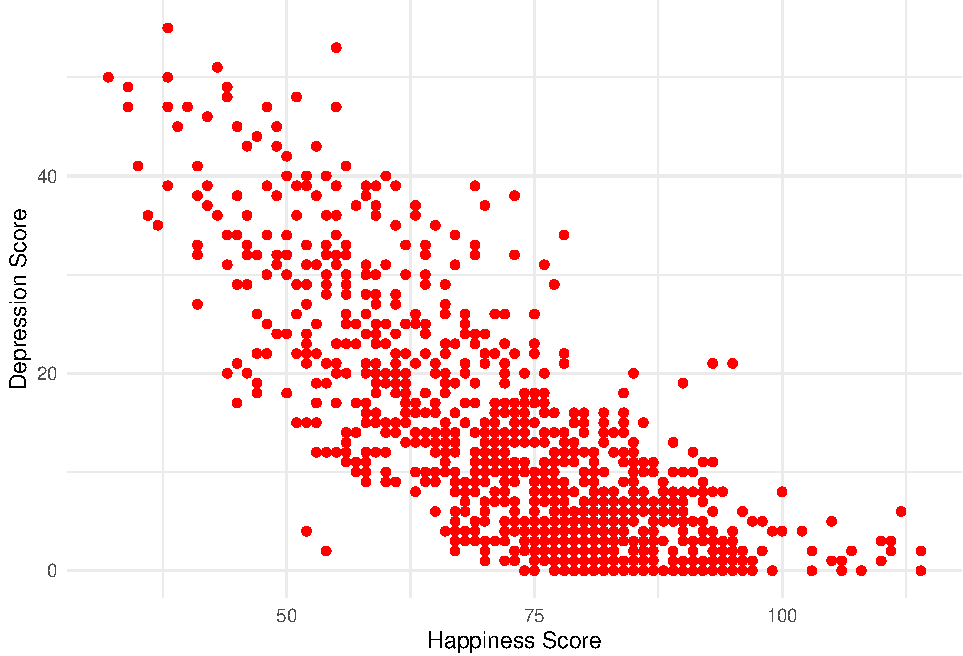
\includegraphics[width=1\linewidth]{08-scatterplots_files/figure-latex/T3-1} \end{center}

\hypertarget{activity-4}{%
\subsection{Activity 4}\label{activity-4}}

Solution

\begin{Shaded}
\begin{Highlighting}[]
\FunctionTok{ggplot}\NormalTok{(all\_dat, }\FunctionTok{aes}\NormalTok{(}\AttributeTok{x =}\NormalTok{ ahiTotal , }\AttributeTok{y =}\NormalTok{ cesdTotal)) }\SpecialCharTok{+} 
  \FunctionTok{geom\_point}\NormalTok{(}\AttributeTok{colour =} \StringTok{"red"}\NormalTok{) }\SpecialCharTok{+}
  \FunctionTok{scale\_x\_continuous}\NormalTok{(}\AttributeTok{name =} \StringTok{"Happiness Score"}\NormalTok{) }\SpecialCharTok{+}
  \FunctionTok{scale\_y\_continuous}\NormalTok{(}\AttributeTok{name =} \StringTok{"Depression Score"}\NormalTok{,}
                     \AttributeTok{limits =} \FunctionTok{c}\NormalTok{(}\DecValTok{0}\NormalTok{,}\DecValTok{60}\NormalTok{)) }\SpecialCharTok{+}
  \FunctionTok{theme\_minimal}\NormalTok{() }\SpecialCharTok{+}
  \FunctionTok{geom\_smooth}\NormalTok{(}\AttributeTok{method =} \StringTok{"lm"}\NormalTok{, }\AttributeTok{formula =}\NormalTok{ y}\SpecialCharTok{\textasciitilde{}}\NormalTok{x)}
\end{Highlighting}
\end{Shaded}

\begin{center}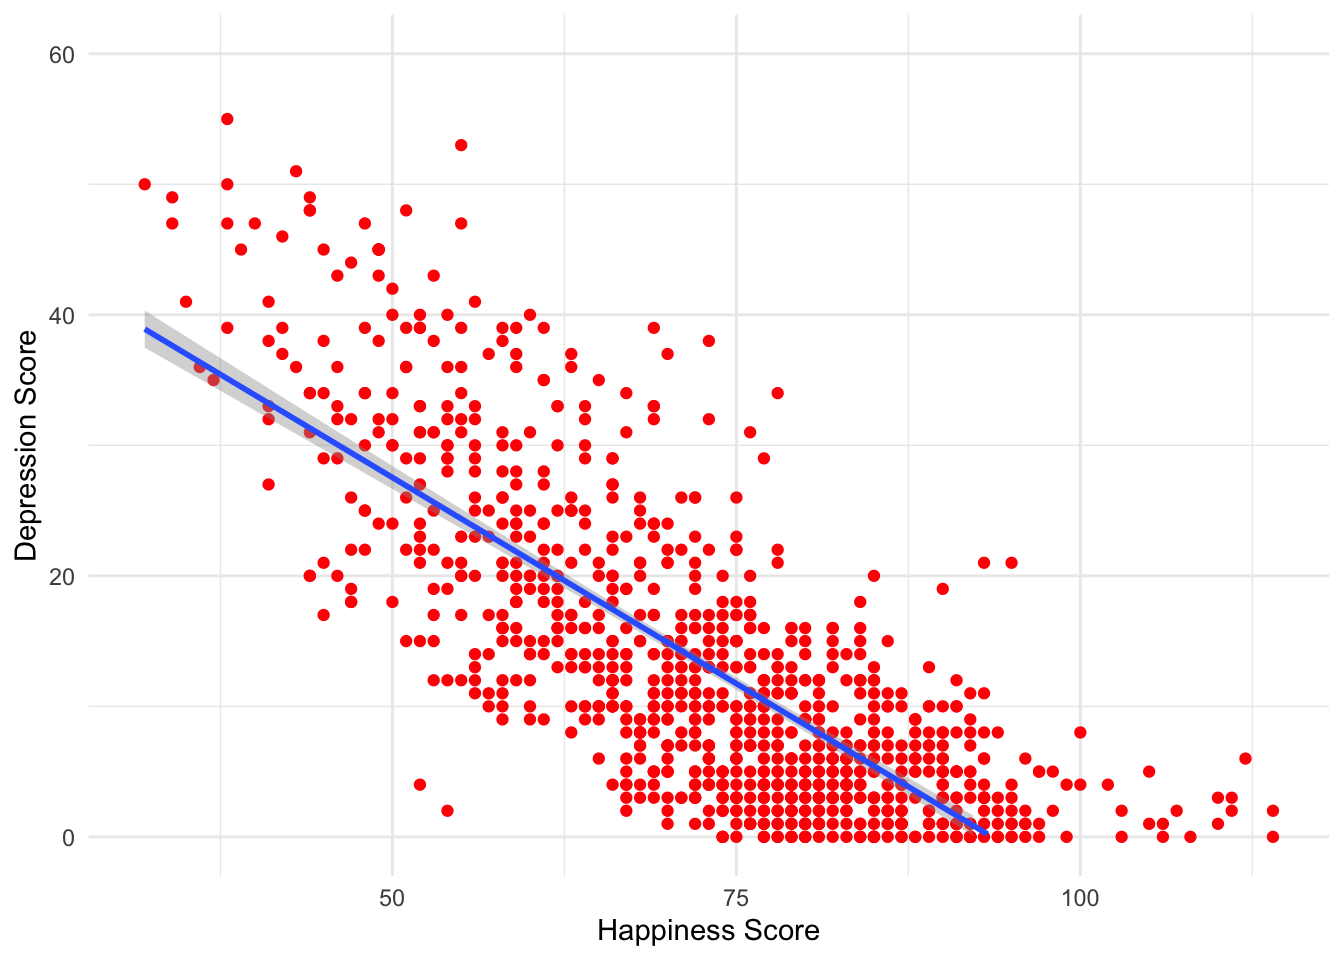
\includegraphics[width=1\linewidth]{08-scatterplots_files/figure-latex/T4s-1} \end{center}

\hypertarget{activity-5}{%
\subsection{Activity 5}\label{activity-5}}

Solution

\begin{Shaded}
\begin{Highlighting}[]
\NormalTok{summarydata }\OtherTok{\textless{}{-}}\NormalTok{ summarydata }\SpecialCharTok{\%\textgreater{}\%}
  \FunctionTok{mutate}\NormalTok{(}\AttributeTok{sex =} \FunctionTok{as.factor}\NormalTok{(sex),}
         \AttributeTok{educ =} \FunctionTok{as.factor}\NormalTok{(educ),}
         \AttributeTok{income =} \FunctionTok{as.factor}\NormalTok{(income))}
\end{Highlighting}
\end{Shaded}

\hypertarget{activity-6-1}{%
\subsection{Activity 6}\label{activity-6-1}}

Solution

\begin{Shaded}
\begin{Highlighting}[]
\FunctionTok{ggplot}\NormalTok{(summarydata, }\FunctionTok{aes}\NormalTok{(}\AttributeTok{x =}\NormalTok{ ahiTotal , }\AttributeTok{y =}\NormalTok{ cesdTotal, }
                        \AttributeTok{colour =}\NormalTok{ educ)) }\SpecialCharTok{+} 
  \FunctionTok{geom\_point}\NormalTok{() }\SpecialCharTok{+}
  \FunctionTok{scale\_x\_continuous}\NormalTok{(}\AttributeTok{name =} \StringTok{"Happiness Score"}\NormalTok{) }\SpecialCharTok{+}
  \FunctionTok{scale\_y\_continuous}\NormalTok{(}\AttributeTok{name =} \StringTok{"Depression Score"}\NormalTok{,}
                     \AttributeTok{limits =} \FunctionTok{c}\NormalTok{(}\DecValTok{0}\NormalTok{,}\DecValTok{60}\NormalTok{)) }\SpecialCharTok{+}
  \FunctionTok{theme\_minimal}\NormalTok{() }\SpecialCharTok{+}
  \FunctionTok{geom\_smooth}\NormalTok{(}\AttributeTok{method =} \StringTok{"lm"}\NormalTok{, }\AttributeTok{formula =}\NormalTok{ y}\SpecialCharTok{\textasciitilde{}}\NormalTok{x) }\SpecialCharTok{+}
  \FunctionTok{scale\_color\_viridis\_d}\NormalTok{(}\AttributeTok{name =} \StringTok{"Education level"}\NormalTok{, }
                       \AttributeTok{labels =} \FunctionTok{c}\NormalTok{(}\StringTok{"Less than Year 12"}\NormalTok{,}
                                  \StringTok{"Year 12"}\NormalTok{,}
                                  \StringTok{"Vocational training"}\NormalTok{,}
                                  \StringTok{"Bachelor’s degree"}\NormalTok{,}
                                  \StringTok{"Postgraduate degree"}\NormalTok{),}
                       \AttributeTok{option =} \StringTok{"E"}\NormalTok{)}
\end{Highlighting}
\end{Shaded}

\begin{center}\includegraphics[width=1\linewidth]{08-scatterplots_files/figure-latex/unnamed-chunk-10-1} \end{center}

\begin{Shaded}
\begin{Highlighting}[]
\FunctionTok{ggplot}\NormalTok{(summarydata, }\FunctionTok{aes}\NormalTok{(}\AttributeTok{x =}\NormalTok{ ahiTotal , }\AttributeTok{y =}\NormalTok{ cesdTotal, }
                        \AttributeTok{colour =}\NormalTok{ income)) }\SpecialCharTok{+} 
  \FunctionTok{geom\_point}\NormalTok{() }\SpecialCharTok{+}
  \FunctionTok{scale\_x\_continuous}\NormalTok{(}\AttributeTok{name =} \StringTok{"Happiness Score"}\NormalTok{) }\SpecialCharTok{+}
  \FunctionTok{scale\_y\_continuous}\NormalTok{(}\AttributeTok{name =} \StringTok{"Depression Score"}\NormalTok{,}
                     \AttributeTok{limits =} \FunctionTok{c}\NormalTok{(}\DecValTok{0}\NormalTok{,}\DecValTok{60}\NormalTok{)) }\SpecialCharTok{+}
  \FunctionTok{theme\_minimal}\NormalTok{() }\SpecialCharTok{+}
  \FunctionTok{geom\_smooth}\NormalTok{(}\AttributeTok{method =} \StringTok{"lm"}\NormalTok{, }\AttributeTok{formula =}\NormalTok{ y}\SpecialCharTok{\textasciitilde{}}\NormalTok{x) }\SpecialCharTok{+}
  \FunctionTok{scale\_color\_viridis\_d}\NormalTok{(}\AttributeTok{name =} \StringTok{"Income"}\NormalTok{, }
                       \AttributeTok{labels =} \FunctionTok{c}\NormalTok{(}\StringTok{"Below average"}\NormalTok{,}
                                  \StringTok{"Average"}\NormalTok{,}
                                  \StringTok{"Above average"}\NormalTok{))}
\end{Highlighting}
\end{Shaded}

\begin{center}\includegraphics[width=1\linewidth]{08-scatterplots_files/figure-latex/unnamed-chunk-11-1} \end{center}

\hypertarget{activity-7}{%
\subsection{Activity 7}\label{activity-7}}

Solution

\begin{Shaded}
\begin{Highlighting}[]
\NormalTok{summarydata }\OtherTok{\textless{}{-}} \FunctionTok{mutate}\NormalTok{(summarydata, }\AttributeTok{severity =}\NormalTok{ cesdTotal }\SpecialCharTok{\textgreater{}=} \DecValTok{18}\NormalTok{)}
\end{Highlighting}
\end{Shaded}

\hypertarget{aq-data-and-recap}{%
\chapter{AQ data and recap}\label{aq-data-and-recap}}

Welcome back to Psych 1B! This semester we're going to build on the data skills you developed in the first semester by adding in a couple of new data wrangling functions, running probability simulations in preparation for statistics in level 2, and analysing your own data for the group project.

\begin{info}
If you haven't yet installed R on your own machine, we strongly
encourage you to do so as it means that a) you're not reliant on the
server b) you don't need to be connected to the internet to use R and c)
it makes it much easier to check your homework files before you submit
them. There is more info in the
\href{https://psyteachr.github.io/ug1-practical/installing-r-on-your-computer-1.html}{Appendix}
and you can also attend a GTA support session if you need help.
\end{info}

It would be nice to always get data formatted in the way that you want it, but one of the challenges as a scientist is dealing with Other People's Data. People often structure data in ways that is convenient for data entry, but not very convenient for data analysis, and so, much effort must be expended 'wrangling' data into shape before you can do more interesting things with it. Additionally, performing analyses often requires pulling together data obtained from different sources: you have done this in semester 1 by combining the participant information with the depression and happiness data. In this semester, we are going to give you some tips on how to structure data, and introduce strategies for transforming and combining data from different sources.

\hypertarget{autism-quotient-data}{%
\section{Autism-quotient data}\label{autism-quotient-data}}

For Psych 1B we're going to use a different dataset for our exercises based upon data that was collected using SurveyMonkey but that has has simulated variables added for the purposes of these exercises (gender was missing, so we have added this in). For this research project, participants completed the short 10-item version of the Autism-Spectrum Quotient (AQ) (Baron-Cohen, Wheelwright, Skinner, Martin, \& Clubley, 2001), which is designed to measure autistic traits in adults. The items for the questionnaire are shown below.

Table 1: The ten items on the AQ-10.

\begin{tabular}{l|l}
\hline
Q\_No & Question\\
\hline
Q 1 & I often notice small sounds when others do not.\\
\hline
Q 2 & I usually concentrate more on the whole picture, rather than small details.\\
\hline
Q 3 & I find it easy to do more than one thing at once.\\
\hline
Q 4 & If there is an interruption, I can switch back to what I was doing very quickly.\\
\hline
Q 5 & I find it easy to read between the lines when someone is talking to me.\\
\hline
Q 6 & I know how to tell if someone listening to me is getting bored.\\
\hline
Q 7 & When I’m reading a story, I find it difficult to work out the characters’ intentions.\\
\hline
Q 8 & I like to collect information about categories of things.\\
\hline
Q 9 & I find it easy to work out what someone is thinking or feeling just by looking at their face.\\
\hline
Q 10 & I find it difficult to work out people’s intentions.\\
\hline
\end{tabular}

Responses to each item were measured on a four-point scale: Definitely Disagree, Slightly Disagree, Slightly Agree, Definitely Agree. One of the issues with conducting research using surveys is that if we don't design them carefully, our data may be affected by response bias. One type of response bias is \textbf{acquiescence bias}, which is the finding that people have a tendancy to agree with all statements. To try and minimise the impact of this, many questionnaires will \textbf{reverse-code} some of the questions so that a positive response means agreeing with one question but disagreeing with another.

\begin{itemize}
\tightlist
\item
  Read through the questions. Type the number of one of the items where you think \textbf{agreeing} with the item would mean the participant displayed autistic traits
\item
  Now type the number of one of the items where you think \textbf{disagreeing} with the item would mean the participant displayed autistic traits
\end{itemize}

For those items where agreeing with the item means a higher autistic quotient (AQ) score, participants recieve a score of 1 if they answer ``Slightly agree'' or ``Agree''. This is called \textbf{forward scoring}. For those items where disagreeing with the item means a higher AQ score, participants recieve a score of 1 if they answer ``Slightly disagree'' or ``Disagree''. This is know as \textbf{reverse coding}.

The AQ score for each participant is the total score (i.e., the sum) of all 10 questions. The higher the AQ score, the more 'autistic traits' they are assumed to exhibit and it is this score we are interested in.

\hypertarget{activity-1-download-the-data}{%
\section{Activity 1: Download the data}\label{activity-1-download-the-data}}

\begin{itemize}
\tightlist
\item
  Download the \texttt{Psych\ 1B} zip file.
\item
  If you're working on your computer, extract the files, and make sure it is saved somewhere sensible. If you're one of those people who has 20 versions of the same file, stop being that person and tidy up your files.
\item
  If you're working on the server, upload the zip file to the server. It will automatically unzip it for you. As above, tidy up your server files if necessary.
\end{itemize}

\hypertarget{activity-2-open-a-new-markdown-document}{%
\section{Activity 2: Open a new Markdown document}\label{activity-2-open-a-new-markdown-document}}

In Psych 1A, we provided the Markdown documents for you in the form of stub files. From this point on, you're going to create and save your own.

\begin{itemize}
\tightlist
\item
  Open R Studio and set the working directory to your Psych 1B folder. If this has worked, you should see the csv files you just downloaded in the file pane in the bottom right of R Studio.\\
\item
  To open a new R Markdown document click the `new item' icon and then click `R Markdown'. You will be prompted to give it a title, call it ``AQ data and recap''. Also, change the author name to your GUID as this will be good practice for the homework. Keep the output format as HTML.
\item
  Once you've opened a new document be sure to save it by clicking \texttt{File} -\textgreater{} \texttt{Save\ as}. Name this file ``AQ data and recap''. If you've set the working directory correctly, you should now see this file appear in your file viewer pane.
\end{itemize}

\begin{figure}

{\centering \includegraphics[width=1\linewidth]{images/markdown_new} 

}

\caption{Opening a new R Markdown document}\label{fig:img-new-markdownb}
\end{figure}

\hypertarget{activity-3-create-a-new-code-chunk}{%
\section{Activity 3: Create a new code chunk}\label{activity-3-create-a-new-code-chunk}}

Let's recap how to use Markdown. When you first open a new R Markdown document you will see a bunch of default welcome text. Do the following steps:

\begin{itemize}
\tightlist
\item
  Delete \textbf{everything} below line 7\\
\item
  On line 8 type ``Activity 3''\\
\item
  Click \texttt{Insert} -\textgreater{} \texttt{R}
\end{itemize}

\begin{figure}

{\centering \includegraphics[width=1\linewidth]{images/markdown-code_chunks} 

}

\caption{New R chunk}\label{fig:img-new-chunkb}
\end{figure}

You should create a new code chunk \textbf{for each activity} or each analysis step (like there was in the stub files from 1A) and make sure there is a description of what the code is doing. This will make it easier to read your Markdown and find where any errors in the code are. \textbf{Do not put all of your code in one big chunk.}

\hypertarget{activity-4-load-in-the-data}{%
\section{Activity 4: Load in the data}\label{activity-4-load-in-the-data}}

\begin{itemize}
\tightlist
\item
  Type and run the code that loads the \texttt{tidyverse} package.
\item
  Use \texttt{read\_csv()} to load in the data. you should create three objects \texttt{responses}, \texttt{scoring} and \texttt{qformats} that contain the respective data. If you need help remembering how to load in data files, check Loading Data.
\end{itemize}

\begin{info}
The solutions are at the bottom if you need them. However, as you'll
discover in your memory and learning lectures, you'll learn more if you
try and retrieve the code from memory. There were a couple of comments
in the 1A EvaSys that said some of you felt like you were just copying
and pasting - this can only be true if \textbf{you choose} to copy and
paste.
\end{info}

\hypertarget{activity-5-look-at-the-data}{%
\section{Activity 5: Look at the data}\label{activity-5-look-at-the-data}}

\begin{itemize}
\item
  View each of the three datasets by clicking on their name in the environment.
\item
  Check each object by using \texttt{summary()}, e.g., \texttt{summary(qformats)}.
\item
  \textbf{responses} contains the actual data from the survey. There is a participant Id column and then the rest of the columns contain the responses associated with that participant for each of the 10 questions (Q1, Q2, Q3, \ldots, Q10).\\
\item
  \textbf{scoring} contains the scoring information that we described above, that is, whether a question should be given a score of 1 or 0 for forward and reverse coded items for each possible response.\\
\item
  \textbf{qformats} contains a list of whether each question is forward or reverse coded.
\end{itemize}

\hypertarget{thinking-through-the-problem}{%
\section{Thinking through the problem}\label{thinking-through-the-problem}}

In order to get a total AQ score for each participant, we need to combine the information from all three files, that is, we need to know the participants response and then how to score it. We technically \emph{could} score the data by hand. However, there are 66 participants in this dataset with each participant providing 10 responses. This means we would have to manually tidy up 660 responses.

Not only would this be a horribly mind-numbing task, it is also one in which you would be prone to make errors. Even if you were 99\% accurate, you would still get about 7 of the scores wrong. Worst of all, this approach does not scale beyond small datasets. When you analyse the data from your group project, there will likely be thousands of participants and you don't have time to do these by hand!

\begin{center}\rule{0.5\linewidth}{0.5pt}\end{center}

\begin{itemize}
\tightlist
\item
  Pause here and think about how you might calculate AQ scores for each participant. What are the necessary steps?
\end{itemize}

\begin{center}\rule{0.5\linewidth}{0.5pt}\end{center}

Let's imagine we are doing the task by hand so that we understand the logic. Once that logic is clear, we'll go through it again and show you how to write the script to make it happen.

Let's take stock of what we know. First, we know that there are two question formats, and that questions Q1, Q7, Q8, and Q10 are scored according to format F and questions Q2, Q3, Q4, Q5, Q6, and Q9 are scored according to format R. This is the information that is currently stored in \texttt{qformats}:

\begin{tabular}{l|l}
\hline
Question & QFormat\\
\hline
Q 1 & F\\
\hline
Q 2 & R\\
\hline
Q 3 & R\\
\hline
Q 4 & R\\
\hline
Q 5 & R\\
\hline
Q 6 & R\\
\hline
Q 7 & F\\
\hline
Q 8 & F\\
\hline
Q 9 & R\\
\hline
Q 10 & F\\
\hline
\end{tabular}

We also know that for format \textbf{F}, we award a point for \textbf{agree}, zero for \textbf{disagree}. For format \textbf{R}, a point for \textbf{disagree}, zero for \textbf{agree}. This is the information that is currently stored in \texttt{scoring}:

\begin{tabular}{l|l|r}
\hline
QFormat & Response & Score\\
\hline
F & Definitely Agree & 1\\
\hline
F & Slightly Agree & 1\\
\hline
F & Slightly Disagree & 0\\
\hline
F & Definitely Disagree & 0\\
\hline
R & Definitely Agree & 0\\
\hline
R & Slightly Agree & 0\\
\hline
R & Slightly Disagree & 1\\
\hline
R & Definitely Disagree & 1\\
\hline
\end{tabular}

Finally, we would need to look at the responses from each participant and then give them the correct score for the format of the question. Let's walk through the example with the first participant. For this participant (Id = 16), we have the following responses:

\begin{tabular}{l|l}
\hline
Question & Participant 16 Response\\
\hline
Q 1 & Slightly Disagree\\
\hline
Q 2 & Definitely Agree\\
\hline
Q 3 & Slightly Disagree\\
\hline
Q 4 & Definitely Disagree\\
\hline
Q 5 & Slightly Agree\\
\hline
Q 6 & Slightly Agree\\
\hline
Q 7 & Slightly Agree\\
\hline
Q 8 & Definitely Disagree\\
\hline
Q 9 & Slightly Agree\\
\hline
Q 10 & Slightly Agree\\
\hline
\end{tabular}

Note that we have re-formatted the responses so that each response is in a separate row, rather than having all of the responses in a single row, as they are in \texttt{responses}. We have reshaped the data from its original \textbf{wide format} to \textbf{long format}. This format is called long because instead of having just one row for each participant, we now have one row for each data point and so 10 rows for each participant.

While this format makes it less easy to read the whole dataset in with a single glance, it actually ends up being much easier to deal with, because 'Question' is a now a single variable whose levels are Q1, Q2, \ldots, Q10, and 'Response' is also now a single variable. Most functions that you will be working with in R will expect your data to be in long rather than wide format.

Let's now look up the format for each question:

\begin{tabular}{l|l|l}
\hline
Question & Participant 16 Response & QFormat\\
\hline
Q 1 & Slightly Disagree & F\\
\hline
Q 2 & Definitely Agree & R\\
\hline
Q 3 & Slightly Disagree & R\\
\hline
Q 4 & Definitely Disagree & R\\
\hline
Q 5 & Slightly Agree & R\\
\hline
Q 6 & Slightly Agree & R\\
\hline
Q 7 & Slightly Agree & F\\
\hline
Q 8 & Definitely Disagree & F\\
\hline
Q 9 & Slightly Agree & R\\
\hline
Q 10 & Slightly Agree & F\\
\hline
\end{tabular}

And now that we have the format and the response, we can look up the scores:

\begin{tabular}{l|l|l|r}
\hline
Question & Participant 16 Response & QFormat & Score\\
\hline
Q 1 & Slightly Disagree & F & 0\\
\hline
Q 2 & Definitely Agree & R & 0\\
\hline
Q 3 & Slightly Disagree & R & 1\\
\hline
Q 4 & Definitely Disagree & R & 1\\
\hline
Q 5 & Slightly Agree & R & 0\\
\hline
Q 6 & Slightly Agree & R & 0\\
\hline
Q 7 & Slightly Agree & F & 1\\
\hline
Q 8 & Definitely Disagree & F & 0\\
\hline
Q 9 & Slightly Agree & R & 0\\
\hline
Q 10 & Slightly Agree & F & 1\\
\hline
\end{tabular}

Then we just add up the scores, which yields an AQ score of 4 for participant 16. We would then repeat this logic for the remaining 65 participants. Anyone fancy doing this for a big data set?!

Due to the large margin for error in carrying out this task by hand, it's important to learn how to make the computer do the dirty work. The computer won't make mistakes and will free up your mind to focus on the bigger issues in your research.

\hypertarget{activity-5-recap}{%
\section{Activity 5: Recap}\label{activity-5-recap}}

Finally, let's refresh your memory of some of the important tidyverse functions before we delve into anything new.

\begin{itemize}
\tightlist
\item
  What function would you use to keep just the columns Q1 and Q2 in \texttt{responses}? filterselectobjectQ1:Q2
\item
  What function would you use to keep just the data from participant 16 in \texttt{reponses}? filterselectsummariseobservation
\item
  What function would you use to add up the total score for participant 16? filterinner\_joinsummarisescore
\item
  What function would you use to join together \texttt{qformats} and \texttt{scoring}? inner\_joinjoinjoin\_innerobject\_join
\end{itemize}

\hypertarget{activity-solutions---aq-data-and-recap}{%
\section{Activity solutions - AQ data and recap}\label{activity-solutions---aq-data-and-recap}}

\hypertarget{activity-4-1}{%
\subsection{Activity 4}\label{activity-4-1}}

Solution

\begin{Shaded}
\begin{Highlighting}[]
\FunctionTok{library}\NormalTok{(tidyverse)}
\NormalTok{scoring }\OtherTok{\textless{}{-}} \FunctionTok{read\_csv}\NormalTok{ (}\StringTok{"scoring.csv"}\NormalTok{)}
\NormalTok{responses }\OtherTok{\textless{}{-}} \FunctionTok{read\_csv}\NormalTok{(}\StringTok{"responses.csv"}\NormalTok{)}
\NormalTok{qformats }\OtherTok{\textless{}{-}} \FunctionTok{read\_csv}\NormalTok{(}\StringTok{"qformats.csv"}\NormalTok{)}
\end{Highlighting}
\end{Shaded}

\hypertarget{reshaping-data}{%
\chapter{Reshaping data}\label{reshaping-data}}

Let's continue what we started in AQ Data and Recap by hand but now using R to calculate a score for each participant.

\hypertarget{activity-1-load-in-the-data}{%
\section{Activity 1: Load in the data}\label{activity-1-load-in-the-data}}

\begin{itemize}
\tightlist
\item
  Open a new R markdown document, name it ``Reshaping Data'' and save it in your Data Skills folder.
\item
  Set the working directory to your Data Skills folder.
\item
  Type and run the code that loads the \texttt{tidyverse} package.
\item
  Use \texttt{read\_csv()} to load in the data. you should create three objects \texttt{responses}, \texttt{scoring} and \texttt{qformats} that contain the respective data.
\end{itemize}

\hypertarget{activity-2-pivot_longer}{%
\section{\texorpdfstring{Activity 2: \texttt{pivot\_longer()}}{Activity 2: pivot\_longer()}}\label{activity-2-pivot_longer}}

The first step is to transform the data from wide format to long format. To do this, we will use the function \texttt{pivot\_longer()}. \texttt{pivot\_longer()} takes multiple columns and collapses them so that each unique variable has it's own column and has four main arguments:

\begin{itemize}
\tightlist
\item
  \texttt{data} is the name of the object you want to transform
\item
  \texttt{names\_to} is the name of the new column that you will create that will contain the names of the original wide format columns
\item
  \texttt{values\_to} is the name of the column that will contain the existing values.
\item
  \texttt{cols} are the original columns you want to collapse.
\end{itemize}

These functions can seem a bit abstract and it is better to show than tell. Run the below code in a new code chunk and then compare how \texttt{rlong} looks compared to \texttt{responses} and see if you can figure out what effect each argument had.

\begin{Shaded}
\begin{Highlighting}[]
\NormalTok{rlong }\OtherTok{\textless{}{-}} \FunctionTok{pivot\_longer}\NormalTok{(}\AttributeTok{data =}\NormalTok{ responses, }
                      \AttributeTok{names\_to =} \StringTok{"Question"}\NormalTok{,  }
                      \AttributeTok{values\_to =} \StringTok{"Response"}\NormalTok{,}
                      \AttributeTok{cols =}\NormalTok{ Q1}\SpecialCharTok{:}\NormalTok{Q10)}
\end{Highlighting}
\end{Shaded}

You have now created a tibble with 660 observations and 3 variables; 10 observations per 66 participants and 3 variables. Let's recreate the example from the AQ Data and Recap and only use \textbf{one participant}. We can do that by using \texttt{filter()} (which you used last semester) to create a new object called \texttt{rlong\_16.}

\hypertarget{activity-3-filter}{%
\section{\texorpdfstring{Activity 3: \texttt{filter()}}{Activity 3: filter()}}\label{activity-3-filter}}

\begin{center}\rule{0.5\linewidth}{0.5pt}\end{center}

\textbf{Pause here and test your knowledge}

\begin{itemize}
\tightlist
\item
  What does \texttt{filter()} do?
\end{itemize}

Retains or removes variablesRetains or removes observations

\begin{center}\rule{0.5\linewidth}{0.5pt}\end{center}

\begin{itemize}
\tightlist
\item
  Create a new object called \texttt{rlong\_16} that uses \texttt{filter()} to keep only the data from participant Id 16.
\end{itemize}

\begin{danger}
Every year, the biggest problem with these exercises is typos caused by
not paying attention to the exact spelling and capitalisation. Remember,
\texttt{Question} is not the same as \texttt{question},
\texttt{Response} is not the same as \texttt{response}, and \texttt{Id}
is not the same as \texttt{ID.}
\end{danger}

\hypertarget{activity-4-inner_join}{%
\section{\texorpdfstring{Activity 4: \texttt{inner\_join()}}{Activity 4: inner\_join()}}\label{activity-4-inner_join}}

The next step is to match each question with its format (F or R) that is stored in \textbf{qformats}. That is, we need to join together the two objects using \texttt{inner\_join()} like we did in Psych 1A.

\begin{itemize}
\tightlist
\item
  Create a new object called \texttt{rlong\_16\_join} that uses \texttt{inner\_join()} to join together \texttt{rlong\_16} and \texttt{qformats}by their common column.
\item
  If you get the error \texttt{Error:\ by\ can\textquotesingle{}t\ contain\ join\ column\ XXXX\ which\ is\ missing\ from\ LHS} it means that you have made a typo. Check the exact spelling and capitalisation of the variable names.
\end{itemize}

\begin{center}\rule{0.5\linewidth}{0.5pt}\end{center}

\texttt{inner\_join()} matches up rows in the two tables where both tables have the same value for the variable named in the third argument, ``Question''. It then combines the columns from the two tables, copying rows where necessary.

To state it more simply, what it does is the following: For each row in \texttt{rlong}, it checks the value of the column \texttt{Question}, and looks for rows with the same value in \texttt{qformats}, and then essentially combines all of the other columns in the two tables for these matching rows. If there are values that don't match, the rows get dropped. The \texttt{inner\_join()} function is one of the most useful and time-saving operations in data wrangling so keep practising as it will keep reappearing time after time.

\hypertarget{activity-5-another-inner_join}{%
\section{\texorpdfstring{Activity 5: Another \texttt{inner\_join()}}{Activity 5: Another inner\_join()}}\label{activity-5-another-inner_join}}

Now that we have matched up each question with its corresponding format, we can now ``look up'' the corresponding scores in the scoring table based on the format and the response. This means we have to use \texttt{inner\_join()} once again to join \texttt{rlong\_16\_join} with \texttt{scoring}**

\begin{itemize}
\tightlist
\item
  Create a new object named \texttt{scores\_16} that joins together \texttt{rlong\_16\_join} with \texttt{scoring}.
\item
  Be careful to tell R \textbf{all} the columns the two objects have in common. Remember that when you need to specify multiple variables you will need to use the syntax \texttt{by\ =\ c("var1",\ "var2)}.
\item
  The reason we have to do two separate \texttt{inner\_joins()} is because they can only join two tables at once and we have three, so it requires two steps.
\end{itemize}

\hypertarget{activity-6-calculating-the-aq-score}{%
\section{Activity 6: Calculating the AQ score}\label{activity-6-calculating-the-aq-score}}

Now you need to calculate the total AQ score for participant 16.

\begin{itemize}
\tightlist
\item
  Create a new object called \texttt{AQ\_16}. Use \texttt{summarise()} and \texttt{sum()}to add up the numbers in the column \texttt{Score} from \texttt{scores\_16} and call the result of this calculation \texttt{AQ\_score}.
\item
  This is a difficult task to do from memory but try it anyway - if you get anywhere near the right solution you're doing extremely well!
\end{itemize}

\hypertarget{activity-7-calculating-all-scores}{%
\section{Activity 7: Calculating all scores}\label{activity-7-calculating-all-scores}}

Next we're going to do the same thing but for \textbf{all} participants. The first two steps are the same but we just use the full data \texttt{rlong} rather than the filtered dataset.

\begin{itemize}
\tightlist
\item
  Run the below code in a new code chunk.
\end{itemize}

\begin{Shaded}
\begin{Highlighting}[]
\NormalTok{rlong\_join }\OtherTok{\textless{}{-}} \FunctionTok{inner\_join}\NormalTok{(rlong, qformats, }\StringTok{"Question"}\NormalTok{)}
\NormalTok{scores }\OtherTok{\textless{}{-}} \FunctionTok{inner\_join}\NormalTok{(rlong\_join, scoring, }\FunctionTok{c}\NormalTok{(}\StringTok{"QFormat"}\NormalTok{, }\StringTok{"Response"}\NormalTok{))}
\end{Highlighting}
\end{Shaded}

The final part of calculating the scores requires an extra step because now we don't just want to calculate one score, we want to calculate a score \textbf{for each participant} which means that we need to use \texttt{group\_by()} to group by \texttt{Id}. We're not going to use it in this chapter but we also want our object to show us the participant's gender so we will also add \texttt{gender} to the grouping. If you want to refresh your memory about how \texttt{group\_by()} works, revise Data Wrangling 1.

\begin{Shaded}
\begin{Highlighting}[]
\NormalTok{scores\_grouped }\OtherTok{\textless{}{-}} \FunctionTok{group\_by}\NormalTok{(scores, Id, gender)}
\NormalTok{AQ\_all }\OtherTok{\textless{}{-}} \FunctionTok{summarise}\NormalTok{(scores\_grouped, }\AttributeTok{total\_score =} \FunctionTok{sum}\NormalTok{(Score))}
\end{Highlighting}
\end{Shaded}

\hypertarget{activity-8-visualisation}{%
\section{Activity 8: Visualisation}\label{activity-8-visualisation}}

Finally, use \texttt{ggplot()} and \texttt{geom\_histogram()} to make a histogram of all the total AQ scores. Try and make it look pretty by changing the axis labels and the theme. You can check the solution code to see how the below example was made, but you can make yours look different.

\begin{itemize}
\tightlist
\item
  Hint 1: \texttt{ggplot(data,\ aes(x))\ +\ geom\_histogram()}
\item
  Hint 2: Add \texttt{binwidth\ =\ 1} to \texttt{geom\_histogram()} to change the width of the bars.
\end{itemize}

\begin{figure}

{\centering \includegraphics[width=1\linewidth]{10-reshaping-data_files/figure-latex/unnamed-chunk-5-1} 

}

\caption{Histogram of total AQ scores}\label{fig:unnamed-chunk-5}
\end{figure}

\hypertarget{activity-solutions---reshping-data}{%
\section{Activity solutions - Reshping data}\label{activity-solutions---reshping-data}}

\hypertarget{activity-1-3}{%
\subsection{Activity 1}\label{activity-1-3}}

Solution

\begin{Shaded}
\begin{Highlighting}[]
\FunctionTok{library}\NormalTok{(tidyverse)}
\NormalTok{scoring }\OtherTok{\textless{}{-}} \FunctionTok{read\_csv}\NormalTok{ (}\StringTok{"scoring.csv"}\NormalTok{)}
\NormalTok{responses }\OtherTok{\textless{}{-}} \FunctionTok{read\_csv}\NormalTok{(}\StringTok{"responses.csv"}\NormalTok{)}
\NormalTok{qformats }\OtherTok{\textless{}{-}} \FunctionTok{read\_csv}\NormalTok{(}\StringTok{"qformats.csv"}\NormalTok{)}
\end{Highlighting}
\end{Shaded}

\hypertarget{activity-3-2}{%
\subsection{Activity 3}\label{activity-3-2}}

Solution

\begin{Shaded}
\begin{Highlighting}[]
\NormalTok{rlong\_16 }\OtherTok{\textless{}{-}} \FunctionTok{filter}\NormalTok{(rlong, Id }\SpecialCharTok{==} \DecValTok{16}\NormalTok{)}
\end{Highlighting}
\end{Shaded}

\hypertarget{activity-4-2}{%
\subsection{Activity 4}\label{activity-4-2}}

Solution

\begin{Shaded}
\begin{Highlighting}[]
\NormalTok{rlong\_16\_join }\OtherTok{\textless{}{-}} \FunctionTok{inner\_join}\NormalTok{(rlong\_16, qformats, }\StringTok{"Question"}\NormalTok{)}
\end{Highlighting}
\end{Shaded}

\hypertarget{activity-5-1}{%
\subsection{Activity 5}\label{activity-5-1}}

Solution

\begin{Shaded}
\begin{Highlighting}[]
\NormalTok{scores\_16 }\OtherTok{\textless{}{-}} \FunctionTok{inner\_join}\NormalTok{(rlong\_16\_join, scoring, }\FunctionTok{c}\NormalTok{(}\StringTok{"QFormat"}\NormalTok{, }\StringTok{"Response"}\NormalTok{))}
\end{Highlighting}
\end{Shaded}

\hypertarget{activity-6-2}{%
\subsection{Activity 6}\label{activity-6-2}}

Solution

\begin{Shaded}
\begin{Highlighting}[]
\NormalTok{AQ\_16 }\OtherTok{\textless{}{-}} \FunctionTok{summarise}\NormalTok{(scores\_16, }\AttributeTok{AQ\_score =} \FunctionTok{sum}\NormalTok{(Score))}
\end{Highlighting}
\end{Shaded}

\hypertarget{activity-8}{%
\subsection{Activity 8}\label{activity-8}}

Solution

\begin{Shaded}
\begin{Highlighting}[]
\FunctionTok{ggplot}\NormalTok{(AQ\_all, }\FunctionTok{aes}\NormalTok{(}\AttributeTok{x =}\NormalTok{ total\_score)) }\SpecialCharTok{+}
  \FunctionTok{geom\_histogram}\NormalTok{(}\AttributeTok{binwidth =} \DecValTok{1}\NormalTok{, }\AttributeTok{colour =} \StringTok{"black"}\NormalTok{, }\AttributeTok{fill =} \StringTok{"grey"}\NormalTok{) }\SpecialCharTok{+}
  \FunctionTok{theme\_minimal}\NormalTok{()}\SpecialCharTok{+}
  \FunctionTok{scale\_x\_continuous}\NormalTok{(}\AttributeTok{name =} \StringTok{"Total AQ Score"}\NormalTok{, }\AttributeTok{breaks =} \FunctionTok{c}\NormalTok{(}\DecValTok{0}\NormalTok{,}\DecValTok{1}\NormalTok{,}\DecValTok{2}\NormalTok{,}\DecValTok{3}\NormalTok{,}\DecValTok{4}\NormalTok{,}\DecValTok{5}\NormalTok{,}\DecValTok{6}\NormalTok{,}\DecValTok{7}\NormalTok{,}\DecValTok{8}\NormalTok{,}\DecValTok{9}\NormalTok{,}\DecValTok{10}\NormalTok{)) }\SpecialCharTok{+}
  \FunctionTok{scale\_y\_continuous}\NormalTok{(}\AttributeTok{name =} \StringTok{"Count"}\NormalTok{)}
\end{Highlighting}
\end{Shaded}

\hypertarget{pipes}{%
\chapter{Pipes}\label{pipes}}

\hypertarget{activity-1-recap}{%
\section{Activity 1: Recap}\label{activity-1-recap}}

In Psych 1A we briefly introduced the concept of \textbf{pipes}, if you'd like to recap what you did, you can \href{https://emilynordmann.github.io/ug1-practical/data-wrangling-1.html\#activity-9-pipes}{find it here}.

Pipes look like this: \texttt{\%\textgreater{}\%}. Pipes allow you to send the output from one function straight into another function. Specifically, they send the result of the function before \texttt{\%\textgreater{}\%} to be the first argument of the function after \texttt{\%\textgreater{}\%}. As usual, it's easier to show, rather than tell so let's look at an example.

In the below example we want to perform some common wrangling steps:

\begin{enumerate}
\def\labelenumi{\arabic{enumi}.}
\tightlist
\item
  Read in the data
\item
  Select the columns we want to retain
\item
  Join together our data files
\item
  Filter out participants so that we just use data from people who are aged 18 years or older
\end{enumerate}

So far, when you've done these steps you've created a new object for each part of the process. The code below should look familiar - once you've loaded in the data to \texttt{demographic} and \texttt{raw\_data}, you then create a new object named \texttt{sel\_data} that stores the output of the \texttt{select()} operation, then you create a new object named \texttt{joined\_data} that uses \texttt{sel\_data} as its input and then finally you create another object called \texttt{final\_data} that uses \texttt{joined\_data} as its input.

Note that the below code is just an example, we don't have any data called \texttt{my\_data} so don't try and run this code, it's just for reading.

\begin{Shaded}
\begin{Highlighting}[]
\NormalTok{demographic }\OtherTok{\textless{}{-}} \FunctionTok{read\_csv}\NormalTok{(}\StringTok{"demographic.csv"}\NormalTok{)}
\NormalTok{raw\_data }\OtherTok{\textless{}{-}} \FunctionTok{read\_csv}\NormalTok{(}\StringTok{"my\_data.csv"}\NormalTok{)}

\NormalTok{sel\_data }\OtherTok{\textless{}{-}} \FunctionTok{select}\NormalTok{(raw\_data, id, score)}
\NormalTok{joined\_data }\OtherTok{\textless{}{-}} \FunctionTok{inner\_join}\NormalTok{(sel\_data, demographic, }\AttributeTok{by =} \StringTok{"id"}\NormalTok{)}
\NormalTok{final\_data }\OtherTok{\textless{}{-}} \FunctionTok{filter}\NormalTok{(joined\_data, age }\SpecialCharTok{\textgreater{}=} \DecValTok{18}\NormalTok{)}
\end{Highlighting}
\end{Shaded}

This code will work, however, there's a more efficient way of doing all of these steps that needs far less typing which means fewer chances to make typos. Additionally, if you create lots of objects, it increases the chances that you might accidentally use the wrong one (e.g., \texttt{rlong} instead of \texttt{rlong2}).

By using pipes, we can reduce the amount of code we write and the number of objects we create.

\begin{itemize}
\tightlist
\item
  Remember, pipes allow you to send the output from one function straight into another function where they are used as the first argument.
\item
  Try and translate the below code into plain English. You can read the \texttt{\%\textgreater{}\%} as \textbf{then}.
\end{itemize}

\begin{Shaded}
\begin{Highlighting}[]
\NormalTok{demographic }\OtherTok{\textless{}{-}} \FunctionTok{read\_csv}\NormalTok{(}\StringTok{"demographic.csv"}\NormalTok{)}
\NormalTok{raw\_data }\OtherTok{\textless{}{-}} \FunctionTok{read\_csv}\NormalTok{(}\StringTok{"my\_data.csv"}\NormalTok{)}

\NormalTok{final\_data }\OtherTok{\textless{}{-}}\NormalTok{ raw\_data }\SpecialCharTok{\%\textgreater{}\%}
  \FunctionTok{select}\NormalTok{(id, score) }\SpecialCharTok{\%\textgreater{}\%}
  \FunctionTok{inner\_join}\NormalTok{(demographic, }\AttributeTok{by =} \StringTok{"id"}\NormalTok{)}
  \FunctionTok{filter}\NormalTok{(age }\SpecialCharTok{\textgreater{}=} \DecValTok{18}\NormalTok{) }
\end{Highlighting}
\end{Shaded}

Solution

Take the object \texttt{raw\_data} \textbf{then} select the columns \texttt{id} and \texttt{score} \textbf{then} join it with the data in \texttt{demographic} by \texttt{id} \textbf{then} filter to only include ages of 18 or greater and save this in an object named \texttt{final\_data}.

Importantly, you don't need to write the entire pipe at once, in fact, it's useful to check that each line works as you intended and then add on the next one to make it easier to spot where errors have come in to your code.

For example you might start with:

\begin{Shaded}
\begin{Highlighting}[]
\NormalTok{final\_data }\OtherTok{\textless{}{-}}\NormalTok{ raw\_data }\SpecialCharTok{\%\textgreater{}\%}
  \FunctionTok{select}\NormalTok{(id, score)}
\end{Highlighting}
\end{Shaded}

Then check the output of \texttt{final\_data} to make sure that it contains the columns you intended to select. Then you would add on another line of the pipe:

\begin{Shaded}
\begin{Highlighting}[]
\NormalTok{final\_data }\OtherTok{\textless{}{-}}\NormalTok{ raw\_data }\SpecialCharTok{\%\textgreater{}\%}
  \FunctionTok{select}\NormalTok{(id, score) }\SpecialCharTok{\%\textgreater{}\%}
  \FunctionTok{inner\_join}\NormalTok{(demographic, }\AttributeTok{by =} \StringTok{"id"}\NormalTok{)}
\end{Highlighting}
\end{Shaded}

And check the output again to make sure that the join had worked properly before adding on the final line.

\begin{Shaded}
\begin{Highlighting}[]
\NormalTok{final\_data }\OtherTok{\textless{}{-}}\NormalTok{ raw\_data }\SpecialCharTok{\%\textgreater{}\%}
  \FunctionTok{select}\NormalTok{(id, score) }\SpecialCharTok{\%\textgreater{}\%}
  \FunctionTok{inner\_join}\NormalTok{(demographic, }\AttributeTok{by =} \StringTok{"id"}\NormalTok{)}
  \FunctionTok{filter}\NormalTok{(age }\SpecialCharTok{\textgreater{}=} \DecValTok{18}\NormalTok{) }
\end{Highlighting}
\end{Shaded}

\begin{danger}
As great as pipes are, there are two main cases when it probably makes
sense to write your code without pipes, and save the results from each
step to separate objects:

\begin{enumerate}
\def\labelenumi{\arabic{enumi}.}
\item
  When the output from a step partway through your pipeline is somehow
  useful. For example, you might want to check that a step worked as
  expected, or the information might be useful again later on.
\item
  When you're completing assessments and we want you to save the output
  from a certain step to a specific variable name (we want to check that
  the step worked properly to be able to give you the mark!).
\end{enumerate}
\end{danger}

Which of the following is a pipe? \%\textgreater\%\textless-\%\textless\%

Where do pipes send the result of the function that precedes the pipe? To the third argument of the 18th function.To the first argument of the next function.To the last argument of the next function.

\hypertarget{activity-2-set-up-1}{%
\section{Activity 2: Set-up}\label{activity-2-set-up-1}}

We're going to load in the AQ data to practice some examples.

\begin{itemize}
\tightlist
\item
  Open a new R Markdown document, name it ``Pipes'' and save it in your Data Skills folder.
\item
  Make sure the working directory is set to your Data Skills folder that has the three AQ .csv files.
\item
  Delete the welcome text and insert a new code chunk.
\item
  Copy, paste, and run the below code into the new code chunk.
\end{itemize}

\begin{Shaded}
\begin{Highlighting}[]
\FunctionTok{library}\NormalTok{(tidyverse)}
\NormalTok{scoring }\OtherTok{\textless{}{-}} \FunctionTok{read\_csv}\NormalTok{ (}\StringTok{"scoring.csv"}\NormalTok{)}
\NormalTok{responses }\OtherTok{\textless{}{-}} \FunctionTok{read\_csv}\NormalTok{(}\StringTok{"responses.csv"}\NormalTok{)}
\NormalTok{qformats }\OtherTok{\textless{}{-}} \FunctionTok{read\_csv}\NormalTok{(}\StringTok{"qformats.csv"}\NormalTok{)}
\end{Highlighting}
\end{Shaded}

\hypertarget{activity-3-example-pipe-1}{%
\section{Activity 3: Example pipe 1}\label{activity-3-example-pipe-1}}

Rewrite the below code to use pipes. The solutions are at the bottom but try and work through it on your own - it can be a bit confusing at first but there will be a moment where it suddenly makes sense and you will find it much easier to write code. Remember that if something is difficult it probably means you're learning more.

\textbf{Hint 1:} You're not creating new objects so you can delete the intermediate object names and save the output straight into the final object name \texttt{scores}.\\
\textbf{Hint 2:} The point of using pipes is that they pipe the output into the first argument of the next function, in other words, you can delete the first argument of the new function.\\
\textbf{Hint 3:} Build the pipe up line-by-line and check it at each stage. The output of the first line of the pipe should look like \texttt{rlong}, the output of the second line should look like \texttt{rlong\_join} and so on.

\begin{Shaded}
\begin{Highlighting}[]
\NormalTok{rlong }\OtherTok{\textless{}{-}} \FunctionTok{pivot\_longer}\NormalTok{(}\AttributeTok{data =}\NormalTok{ responses, }
                      \AttributeTok{names\_to =} \StringTok{"Question"}\NormalTok{,  }
                      \AttributeTok{values\_to =} \StringTok{"Response"}\NormalTok{,}
                      \AttributeTok{cols =}\NormalTok{ Q1}\SpecialCharTok{:}\NormalTok{Q10)}

\NormalTok{rlong\_join }\OtherTok{\textless{}{-}} \FunctionTok{inner\_join}\NormalTok{(rlong, qformats, }\StringTok{"Question"}\NormalTok{)}

\NormalTok{scores }\OtherTok{\textless{}{-}} \FunctionTok{inner\_join}\NormalTok{(rlong\_join, scoring, }\FunctionTok{c}\NormalTok{(}\StringTok{"QFormat"}\NormalTok{, }\StringTok{"Response"}\NormalTok{))}
\end{Highlighting}
\end{Shaded}

\hypertarget{activity-4-example-pipe-2}{%
\section{Activity 4: Example pipe 2}\label{activity-4-example-pipe-2}}

Rewrite the below code to use pipes.

\begin{Shaded}
\begin{Highlighting}[]
\NormalTok{data1 }\OtherTok{\textless{}{-}} \FunctionTok{select}\NormalTok{(scores, }\SpecialCharTok{{-}}\NormalTok{QFormat)}
\NormalTok{data2 }\OtherTok{\textless{}{-}} \FunctionTok{filter}\NormalTok{(data1, Question }\SpecialCharTok{==} \StringTok{"Q1"}\NormalTok{)}
\NormalTok{example\_2 }\OtherTok{\textless{}{-}} \FunctionTok{summarise}\NormalTok{(data2, }\AttributeTok{total\_score =} \FunctionTok{sum}\NormalTok{(Score))}
\end{Highlighting}
\end{Shaded}

\hypertarget{activity-5-example-pipe-3}{%
\section{Activity 5: Example pipe 3}\label{activity-5-example-pipe-3}}

You can also pipe into \texttt{ggplot()}. The below example calculates the total score for each question (not each participant) by grouping it, then using summarise on the grouped data, then making a graph of these scores so that we can see which question participants were most likely to give an answer indicating autistic traits. Rewrite the below code using pipes.

\textbf{Hint 1:} You do not need to save this output to an object.\\
\textbf{Hint 2:} First, write the code that calculates the scores and then pipe into \texttt{ggplot()}\\
\textbf{Hint 3:} The pipe works exactly the same with \texttt{ggplot()}, you can delete the first argument.

\begin{Shaded}
\begin{Highlighting}[]
\NormalTok{data\_group }\OtherTok{\textless{}{-}} \FunctionTok{group\_by}\NormalTok{(scores, Question)}
\NormalTok{question\_scores }\OtherTok{\textless{}{-}} \FunctionTok{summarise}\NormalTok{(data\_group, }\AttributeTok{item\_scores =} \FunctionTok{sum}\NormalTok{(Score))}

\FunctionTok{ggplot}\NormalTok{(question\_scores, }\FunctionTok{aes}\NormalTok{(}\AttributeTok{x =}\NormalTok{ Question, }\AttributeTok{y =}\NormalTok{ item\_scores)) }\SpecialCharTok{+}
  \FunctionTok{geom\_col}\NormalTok{() }\SpecialCharTok{+}
  \FunctionTok{theme\_minimal}\NormalTok{()}
\end{Highlighting}
\end{Shaded}

\begin{figure}

{\centering \includegraphics[width=1\linewidth]{11-pipes_files/figure-latex/unnamed-chunk-10-1} 

}

\caption{Total scores for each AQ question}\label{fig:unnamed-chunk-10}
\end{figure}

\hypertarget{activity-solutions---pipes}{%
\section{Activity solutions - Pipes}\label{activity-solutions---pipes}}

\hypertarget{activity-3-3}{%
\subsection{Activity 3}\label{activity-3-3}}

Solution

\begin{Shaded}
\begin{Highlighting}[]
\NormalTok{scores }\OtherTok{\textless{}{-}} \FunctionTok{pivot\_longer}\NormalTok{(}\AttributeTok{data =}\NormalTok{ responses, }
                      \AttributeTok{names\_to =} \StringTok{"Question"}\NormalTok{,  }
                      \AttributeTok{values\_to =} \StringTok{"Response"}\NormalTok{,}
                      \AttributeTok{cols =}\NormalTok{ Q1}\SpecialCharTok{:}\NormalTok{Q10) }\SpecialCharTok{\%\textgreater{}\%}
  \FunctionTok{inner\_join}\NormalTok{(qformats, }\StringTok{"Question"}\NormalTok{) }\SpecialCharTok{\%\textgreater{}\%}
  \FunctionTok{inner\_join}\NormalTok{(scoring, }\FunctionTok{c}\NormalTok{(}\StringTok{"QFormat"}\NormalTok{, }\StringTok{"Response"}\NormalTok{))}

\CommentTok{\# this also does the same thing but the first line is slightly different}

\NormalTok{scores }\OtherTok{\textless{}{-}}\NormalTok{ responses }\SpecialCharTok{\%\textgreater{}\%}
  \FunctionTok{pivot\_longer}\NormalTok{(}\AttributeTok{names\_to =} \StringTok{"Question"}\NormalTok{,  }
               \AttributeTok{values\_to =} \StringTok{"Response"}\NormalTok{,}
               \AttributeTok{cols =}\NormalTok{ Q1}\SpecialCharTok{:}\NormalTok{Q10) }\SpecialCharTok{\%\textgreater{}\%}
  \FunctionTok{inner\_join}\NormalTok{(qformats, }\StringTok{"Question"}\NormalTok{) }\SpecialCharTok{\%\textgreater{}\%}
  \FunctionTok{inner\_join}\NormalTok{(scoring, }\FunctionTok{c}\NormalTok{(}\StringTok{"QFormat"}\NormalTok{, }\StringTok{"Response"}\NormalTok{))}
\end{Highlighting}
\end{Shaded}

\hypertarget{activity-4-3}{%
\subsection{Activity 4}\label{activity-4-3}}

Solution

\begin{Shaded}
\begin{Highlighting}[]
\NormalTok{example\_2 }\OtherTok{\textless{}{-}} \FunctionTok{select}\NormalTok{(scores, }\SpecialCharTok{{-}}\NormalTok{QFormat) }\SpecialCharTok{\%\textgreater{}\%}
  \FunctionTok{filter}\NormalTok{(Question }\SpecialCharTok{==} \StringTok{"Q1"}\NormalTok{) }\SpecialCharTok{\%\textgreater{}\%}
  \FunctionTok{summarise}\NormalTok{(}\AttributeTok{total\_score =} \FunctionTok{sum}\NormalTok{(Score))}
\end{Highlighting}
\end{Shaded}

\hypertarget{activity-5-2}{%
\subsection{Activity 5}\label{activity-5-2}}

Solution

\begin{Shaded}
\begin{Highlighting}[]
\NormalTok{scores }\SpecialCharTok{\%\textgreater{}\%}
  \FunctionTok{group\_by}\NormalTok{(Question) }\SpecialCharTok{\%\textgreater{}\%}
  \FunctionTok{summarise}\NormalTok{(}\AttributeTok{item\_scores =} \FunctionTok{sum}\NormalTok{(Score)) }\SpecialCharTok{\%\textgreater{}\%}
  \FunctionTok{ggplot}\NormalTok{(}\FunctionTok{aes}\NormalTok{(}\AttributeTok{x =}\NormalTok{ Question, }\AttributeTok{y =}\NormalTok{ item\_scores)) }\SpecialCharTok{+}
  \FunctionTok{geom\_col}\NormalTok{() }\SpecialCharTok{+}
  \FunctionTok{theme\_minimal}\NormalTok{()}
\end{Highlighting}
\end{Shaded}

\hypertarget{mega-pipe}{%
\chapter{Mega pipe}\label{mega-pipe}}

\hypertarget{activity-1-set-up-4}{%
\section{Activity 1: Set-up}\label{activity-1-set-up-4}}

\begin{itemize}
\tightlist
\item
  Open a new R markdown document, name it ``Mega pipe'' and save it in your Data Skills folder.
\item
  Set the working directory to your Data Skills folder.
\item
  Type and run the code that loads the \texttt{tidyverse} package.
\item
  Use \texttt{read\_csv()} to load in the data. you should create three objects \texttt{responses}, \texttt{scoring} and \texttt{qformats} that contain the respective data.
\end{itemize}

\hypertarget{activity-2-mega-pipe}{%
\section{Activity 2: Mega pipe}\label{activity-2-mega-pipe}}

We're going to build on what you learned in Pipes and rewrite all of the code we did in Reshaping Data (which you can see below) using a pipe. As a reminder, the code:

\begin{itemize}
\tightlist
\item
  Transforms the data from wide-form to long-form
\item
  Joins together the three objects by their common columns
\item
  Calculates a total AQ score for each participant
\end{itemize}

\begin{Shaded}
\begin{Highlighting}[]
\NormalTok{rlong }\OtherTok{\textless{}{-}} \FunctionTok{pivot\_longer}\NormalTok{(}\AttributeTok{data =}\NormalTok{ responses, }
                      \AttributeTok{names\_to =} \StringTok{"Question"}\NormalTok{,  }
                      \AttributeTok{values\_to =} \StringTok{"Response"}\NormalTok{,}
                      \AttributeTok{cols =}\NormalTok{ Q1}\SpecialCharTok{:}\NormalTok{Q10)}

\NormalTok{rlong\_join }\OtherTok{\textless{}{-}} \FunctionTok{inner\_join}\NormalTok{(rlong, qformats, }\AttributeTok{by =} \StringTok{"Question"}\NormalTok{)}

\NormalTok{scores }\OtherTok{\textless{}{-}} \FunctionTok{inner\_join}\NormalTok{(rlong\_join, scoring, }\AttributeTok{by =} \FunctionTok{c}\NormalTok{(}\StringTok{"QFormat"}\NormalTok{, }\StringTok{"Response"}\NormalTok{))}

\NormalTok{scores\_grouped }\OtherTok{\textless{}{-}} \FunctionTok{group\_by}\NormalTok{(scores, Id, gender)}

\NormalTok{AQ\_all }\OtherTok{\textless{}{-}} \FunctionTok{summarise}\NormalTok{(scores\_grouped, }\AttributeTok{total\_score =} \FunctionTok{sum}\NormalTok{(Score))}
\end{Highlighting}
\end{Shaded}

\begin{itemize}
\tightlist
\item
  Rewrite the above code using pipes \texttt{\%\textgreater{}\%}. Make sure you have completed Pipes before you attempt this.
\end{itemize}

\hypertarget{activity-3-pipe-plot}{%
\section{Activity 3: Pipe plot}\label{activity-3-pipe-plot}}

Now we've got our total AQ scores, let's use the pipe to make a graph.

\begin{itemize}
\tightlist
\item
  Take \texttt{AQ\_all} \textbf{then} filter it leaving only female participants \textbf{then} use \texttt{ggplot()} to create a histogram of the total scores (you did this in Reshaping Data). If you've done it correctly, it should look like the below (you can change the colours if you like).
\end{itemize}

\begin{figure}

{\centering \includegraphics[width=1\linewidth]{12-more-pipes_files/figure-latex/unnamed-chunk-2-1} 

}

\caption{Histogram of scores for female participants}\label{fig:unnamed-chunk-2}
\end{figure}

Remember this for your group project - rather than creating new objects for each graph you want to make you can just pipe the data you want to display straight into \texttt{ggplot()}.

\hypertarget{activity-4-aq-score-by-gender}{%
\section{Activity 4: AQ score by gender}\label{activity-4-aq-score-by-gender}}

\href{https://www.autism.org.uk/about/what-is/gender.aspx}{More men and boys are currently diagnosed as autistic than women and girls} and there is increasing evidence that there is an over-representation of \href{https://www.ncbi.nlm.nih.gov/pubmed/31260907}{transgender and nonbinary people} in those with autism spectrum disorder (ASD) or who meet the AQ cut-off score for ASD, therefore, it seems sensible to visualise AQ scores by gender (note that this dataset is simulated and that whilst the pattern of results is based on what we would expect from the evidence, these are not real data).

\begin{itemize}
\tightlist
\item
  Using the data in \texttt{AQ\_all}, create a violin-boxplot of the total AQ scores by gender.
\item
  Hint: \texttt{gender} should be on the x-axis, \texttt{total\_score} should be on the y-axis.
\item
  You can use a pipe if you want, but it doesn't make much difference in this activity.
\end{itemize}

Look at the graph and answer the following questions:

\begin{itemize}
\item
  Which group has the lowest median total AQ score? femalemalenonbinary
\item
  Which group has an outlier? femalemalenonbinary
\item
  Which of the following do you think would be an accurate conclusion to draw from the plot?

  \hypertarget{radio_EVVIXIRPKO}{}
  {Women had higher AQ scores than men or nonbinary people} {Men and nonbinary people's scores did not differ much and both had higher AQ scores than women} {Men had higher AQ scores than nonbinary people who had higher scores than women}
\end{itemize}

\hypertarget{activity-5-bad-bar-plots}{%
\section{Activity 5: Bad bar plots}\label{activity-5-bad-bar-plots}}

In the research methods lectures for Psych 1A, we talked about the importance of data visualisation and how different graphs might lead you to make very different conclusions about your data. For this reason, we've taught you how to make violin-boxplots because these show the true distribution of the data, however, it's useful to know how to make bad bar plots so that you can see the difference they make to your own data (but never use them as your only method of visualisation!).

\begin{itemize}
\tightlist
\item
  Copy, paste and run the below code in a new code chunk
\item
  Making a bar chart works a little differently to the other graphs you have made so far. Previously, \texttt{ggplot()} has just visualised the raw data, however, for a bar chart you actually want to visualise a \textbf{summary} of the data, e.g., the mean.
\item
  You can read the \texttt{stat\_summary} code as ``draw a summary of the data, use a bar chart to do so and the function to display on the y-axis should be the mean. Then, draw another summary but this time use an errorbar and the function to apply to the data is standard error of the mean''.
\end{itemize}

\begin{Shaded}
\begin{Highlighting}[]
\NormalTok{AQ\_all }\SpecialCharTok{\%\textgreater{}\%}
  \FunctionTok{ggplot}\NormalTok{(}\FunctionTok{aes}\NormalTok{(}\AttributeTok{x =}\NormalTok{ gender, }\AttributeTok{y =}\NormalTok{ total\_score)) }\SpecialCharTok{+}
  \FunctionTok{stat\_summary}\NormalTok{(}\AttributeTok{geom =} \StringTok{"bar"}\NormalTok{, }\AttributeTok{fun =} \StringTok{"mean"}\NormalTok{) }\SpecialCharTok{+}
  \FunctionTok{stat\_summary}\NormalTok{(}\AttributeTok{geom =} \StringTok{"errorbar"}\NormalTok{, }\AttributeTok{fun.data =} \StringTok{"mean\_se"}\NormalTok{, }\AttributeTok{width =}\NormalTok{ .}\DecValTok{2}\NormalTok{) }\SpecialCharTok{+}
  \FunctionTok{theme\_minimal}\NormalTok{()}
\end{Highlighting}
\end{Shaded}

\begin{figure}

{\centering \includegraphics[width=1\linewidth]{12-more-pipes_files/figure-latex/unnamed-chunk-4-1} 

}

\caption{Bad bar chart of means}\label{fig:unnamed-chunk-4}
\end{figure}

Think back to your interpretation of the violin-boxplot, that men and nonbinary people's scores did not differ much and both had higher AQ scores than women. Would you have concluded the same thing if you had looked at the bar chart?

In this dataset, the outlier in the male group results in the mean score being much higher than the nonbinary mean, it's only through looking at the full distribution with the violin-boxplot that you can accurately intepret the data.

\hypertarget{activity-6-density-plots}{%
\section{Activity 6: Density plots}\label{activity-6-density-plots}}

The final type of visualiation we're going to show you are density plots as they are a useful way of visualising how the distributions of different groups compare to each other. You've actually already seen a density plot - it's the base of a violin plot, however, it can be useful to overlap them.

\begin{itemize}
\tightlist
\item
  Copy, paste, and run the below code in a new code chunk.
\item
  A lot of this code should be familiar to you, most of it is editing the axis labels and the theme.
\item
  Adding \texttt{fill\ =\ gender} tells \texttt{ggplot} to produce different coloured geoms for each level of \texttt{gender}. Try removing \texttt{fill\ =\ gender} and see what happens to the plot.
\item
  \texttt{geom\_density()} is our new geom and tells R to draw the density curve. The argument \texttt{alpha} controls the transparency of the colours, try adjusting this value.
\end{itemize}

\begin{Shaded}
\begin{Highlighting}[]
\FunctionTok{ggplot}\NormalTok{(AQ\_all, }\FunctionTok{aes}\NormalTok{(}\AttributeTok{x =}\NormalTok{ total\_score, }\AttributeTok{fill =}\NormalTok{ gender)) }\SpecialCharTok{+}
  \FunctionTok{geom\_density}\NormalTok{(}\AttributeTok{alpha =}\NormalTok{ .}\DecValTok{3}\NormalTok{) }\SpecialCharTok{+}
  \FunctionTok{theme\_minimal}\NormalTok{() }\SpecialCharTok{+}
  \FunctionTok{scale\_fill\_viridis\_d}\NormalTok{(}\AttributeTok{option =} \StringTok{"D"}\NormalTok{) }\SpecialCharTok{+}
  \FunctionTok{scale\_x\_continuous}\NormalTok{(}\AttributeTok{name =} \StringTok{"Total AQ Score"}\NormalTok{, }\AttributeTok{breaks =} \FunctionTok{c}\NormalTok{(}\DecValTok{1}\NormalTok{,}\DecValTok{2}\NormalTok{,}\DecValTok{3}\NormalTok{,}\DecValTok{4}\NormalTok{,}\DecValTok{5}\NormalTok{,}\DecValTok{6}\NormalTok{,}\DecValTok{7}\NormalTok{,}\DecValTok{8}\NormalTok{,}\DecValTok{9}\NormalTok{,}\DecValTok{10}\NormalTok{)) }\SpecialCharTok{+}
  \FunctionTok{scale\_y\_continuous}\NormalTok{(}\AttributeTok{name =} \StringTok{"Density"}\NormalTok{)}
\end{Highlighting}
\end{Shaded}

\begin{figure}

{\centering \includegraphics[width=1\linewidth]{12-more-pipes_files/figure-latex/unnamed-chunk-5-1} 

}

\caption{Grouped density plot}\label{fig:unnamed-chunk-5}
\end{figure}

The y-axis displays density, i.e., what proportion of the data points fall at each point on the x-axis.

\begin{itemize}
\tightlist
\item
  Approximately what percent of female participants had a total AQ of 2? .3\%3\%30\%
\end{itemize}

Solution

It's important to be able to translate between proportions and percentages, it will make your understanding of statistics and p-values much easier. To translate a proportion into a percentage, you multiply by 100 or move the decimal place two places to the right so a proportion of .5 = 50\%, a proportion of .03 = 3\% and so on.

\hypertarget{activity-7-saving-plots}{%
\section{Activity 7: Saving plots}\label{activity-7-saving-plots}}

Finally, it's useful to be able to save a copy of your plots as an image file so that you can use it in a presentation or word document and to do this we can use the function \texttt{ggsave()}.

There are two ways you can use \texttt{ggsave()}. If you don't tell \texttt{ggsave()} which plot you want to save, by default it will save a copy of \textbf{the last plot you created}. If you've been following this chapter in order, the last plot you created should have been the density plot from Activity 6.

All that \texttt{ggsave()} requires is for you to tell it what file name it should save the plot to and the type of image file you want to create (the below example uses .png but you could also use e.g., .jpeg and other image types).

\begin{itemize}
\tightlist
\item
  Copy, paste and run the below code into a new code chunk.
\item
  Check your Data Skills folder, you should now see the saved image file.
\end{itemize}

\begin{Shaded}
\begin{Highlighting}[]
\FunctionTok{ggsave}\NormalTok{(}\StringTok{"density.png"}\NormalTok{)}
\end{Highlighting}
\end{Shaded}

The default size for an image is 7 x 7, you can change this manually if you think that the dimensions of the plot are not correct or if you need a particular size.

\begin{itemize}
\tightlist
\item
  Copy paste and run the below code to overwrite the image file with new dimensions.
\end{itemize}

\begin{Shaded}
\begin{Highlighting}[]
\FunctionTok{ggsave}\NormalTok{(}\StringTok{"density.png"}\NormalTok{, }\AttributeTok{width =} \DecValTok{10}\NormalTok{, }\AttributeTok{height =} \DecValTok{8}\NormalTok{)}
\end{Highlighting}
\end{Shaded}

The second way of using \texttt{ggsave()} is to save your plot as an object and then tell it which object to write to a file. The below code saves the pipe plot from Activity 3 into an object named \texttt{AQ\_histogram} and then saves it to an image file ``AQ\_histogram.png''.

Note that when you save a plot to an object, it won't display in R Studio. To get it to display you need to type the object name in the console (i.e., \texttt{AQ\_histogram}). The benefit of doing it this way is that if you are making lots of plots, you can't accidentally save the wrong one because you are explicitly specifying which plot to save rather than just saving the last one.

\begin{itemize}
\tightlist
\item
  Copy, paste and run the below code and then check your Data Skills folder for the image file. Resize the plot if you think it needs it.
\end{itemize}

\begin{Shaded}
\begin{Highlighting}[]
\NormalTok{AQ\_histogram }\OtherTok{\textless{}{-}}\NormalTok{ AQ\_all }\SpecialCharTok{\%\textgreater{}\%}
  \FunctionTok{filter}\NormalTok{(gender }\SpecialCharTok{==} \StringTok{"female"}\NormalTok{) }\SpecialCharTok{\%\textgreater{}\%}
  \FunctionTok{ggplot}\NormalTok{(}\FunctionTok{aes}\NormalTok{(}\AttributeTok{x =}\NormalTok{ total\_score)) }\SpecialCharTok{+}
  \FunctionTok{geom\_histogram}\NormalTok{(}\AttributeTok{binwidth =} \DecValTok{1}\NormalTok{, }\AttributeTok{colour =} \StringTok{"black"}\NormalTok{, }\AttributeTok{fill =} \StringTok{"grey"}\NormalTok{) }\SpecialCharTok{+}
  \FunctionTok{theme\_minimal}\NormalTok{()}\SpecialCharTok{+}
  \FunctionTok{scale\_x\_continuous}\NormalTok{(}\AttributeTok{name =} \StringTok{"Total AQ Score (female participants)"}\NormalTok{, }\AttributeTok{breaks =} \FunctionTok{c}\NormalTok{(}\DecValTok{0}\NormalTok{,}\DecValTok{1}\NormalTok{,}\DecValTok{2}\NormalTok{,}\DecValTok{3}\NormalTok{,}\DecValTok{4}\NormalTok{,}\DecValTok{5}\NormalTok{,}\DecValTok{6}\NormalTok{,}\DecValTok{7}\NormalTok{,}\DecValTok{8}\NormalTok{,}\DecValTok{9}\NormalTok{,}\DecValTok{10}\NormalTok{)) }\SpecialCharTok{+}
  \FunctionTok{scale\_y\_continuous}\NormalTok{(}\AttributeTok{name =} \StringTok{"Count"}\NormalTok{)}

\FunctionTok{ggsave}\NormalTok{(}\StringTok{"AQ\_histogram.png"}\NormalTok{, }\AttributeTok{plot =}\NormalTok{ AQ\_histogram)}
\end{Highlighting}
\end{Shaded}

\hypertarget{activity-solutions---mega-pipe}{%
\section{Activity solutions - Mega pipe}\label{activity-solutions---mega-pipe}}

\hypertarget{activity-1-4}{%
\subsection{Activity 1}\label{activity-1-4}}

Solution

\begin{Shaded}
\begin{Highlighting}[]
\FunctionTok{library}\NormalTok{(tidyverse)}
\NormalTok{scoring }\OtherTok{\textless{}{-}} \FunctionTok{read\_csv}\NormalTok{ (}\StringTok{"scoring.csv"}\NormalTok{)}
\NormalTok{responses }\OtherTok{\textless{}{-}} \FunctionTok{read\_csv}\NormalTok{(}\StringTok{"responses.csv"}\NormalTok{)}
\NormalTok{qformats }\OtherTok{\textless{}{-}} \FunctionTok{read\_csv}\NormalTok{(}\StringTok{"qformats.csv"}\NormalTok{)}
\end{Highlighting}
\end{Shaded}

\hypertarget{activity-2-3}{%
\subsection{Activity 2}\label{activity-2-3}}

Solution

\begin{Shaded}
\begin{Highlighting}[]
\NormalTok{AQ\_all }\OtherTok{\textless{}{-}} \FunctionTok{pivot\_longer}\NormalTok{(}\AttributeTok{data =}\NormalTok{ responses, }
                      \AttributeTok{names\_to =} \StringTok{"Question"}\NormalTok{,  }
                      \AttributeTok{values\_to =} \StringTok{"Response"}\NormalTok{,}
                      \AttributeTok{cols =}\NormalTok{ Q1}\SpecialCharTok{:}\NormalTok{Q10) }\SpecialCharTok{\%\textgreater{}\%}
  \FunctionTok{inner\_join}\NormalTok{(qformats, }\AttributeTok{by =} \StringTok{"Question"}\NormalTok{) }\SpecialCharTok{\%\textgreater{}\%}
  \FunctionTok{inner\_join}\NormalTok{(scoring, }\AttributeTok{by =} \FunctionTok{c}\NormalTok{(}\StringTok{"QFormat"}\NormalTok{, }\StringTok{"Response"}\NormalTok{)) }\SpecialCharTok{\%\textgreater{}\%}
  \FunctionTok{group\_by}\NormalTok{(Id, gender) }\SpecialCharTok{\%\textgreater{}\%} 
  \FunctionTok{summarise}\NormalTok{(}\AttributeTok{total\_score =} \FunctionTok{sum}\NormalTok{(Score))}
\end{Highlighting}
\end{Shaded}

\hypertarget{activity-3-4}{%
\subsection{Activity 3}\label{activity-3-4}}

Solution

\begin{Shaded}
\begin{Highlighting}[]
\NormalTok{AQ\_all }\SpecialCharTok{\%\textgreater{}\%}
  \FunctionTok{filter}\NormalTok{(gender }\SpecialCharTok{==} \StringTok{"female"}\NormalTok{) }\SpecialCharTok{\%\textgreater{}\%}
  \FunctionTok{ggplot}\NormalTok{(}\FunctionTok{aes}\NormalTok{(}\AttributeTok{x =}\NormalTok{ total\_score)) }\SpecialCharTok{+}
  \FunctionTok{geom\_histogram}\NormalTok{(}\AttributeTok{binwidth =} \DecValTok{1}\NormalTok{, }\AttributeTok{colour =} \StringTok{"black"}\NormalTok{, }\AttributeTok{fill =} \StringTok{"grey"}\NormalTok{) }\SpecialCharTok{+}
  \FunctionTok{theme\_minimal}\NormalTok{()}\SpecialCharTok{+}
  \FunctionTok{scale\_x\_continuous}\NormalTok{(}\AttributeTok{name =} \StringTok{"Total AQ Score (female participants)"}\NormalTok{, }\AttributeTok{breaks =} \FunctionTok{c}\NormalTok{(}\DecValTok{0}\NormalTok{,}\DecValTok{1}\NormalTok{,}\DecValTok{2}\NormalTok{,}\DecValTok{3}\NormalTok{,}\DecValTok{4}\NormalTok{,}\DecValTok{5}\NormalTok{,}\DecValTok{6}\NormalTok{,}\DecValTok{7}\NormalTok{,}\DecValTok{8}\NormalTok{,}\DecValTok{9}\NormalTok{,}\DecValTok{10}\NormalTok{)) }\SpecialCharTok{+}
  \FunctionTok{scale\_y\_continuous}\NormalTok{(}\AttributeTok{name =} \StringTok{"Count"}\NormalTok{)}
\end{Highlighting}
\end{Shaded}

\hypertarget{activity-4-4}{%
\subsection{Activity 4}\label{activity-4-4}}

Solution

\begin{Shaded}
\begin{Highlighting}[]
\FunctionTok{ggplot}\NormalTok{(AQ\_all, }\FunctionTok{aes}\NormalTok{(gender, total\_score)) }\SpecialCharTok{+}
  \FunctionTok{geom\_violin}\NormalTok{(}\AttributeTok{trim =} \ConstantTok{FALSE}\NormalTok{) }\SpecialCharTok{+}
  \FunctionTok{geom\_boxplot}\NormalTok{(}\AttributeTok{width =}\NormalTok{ .}\DecValTok{2}\NormalTok{) }\SpecialCharTok{+}
  \FunctionTok{theme\_minimal}\NormalTok{()}
\end{Highlighting}
\end{Shaded}

\hypertarget{intro-to-probability}{%
\chapter{Intro to Probability}\label{intro-to-probability}}

In the Psych 1A Research Methods lectures, we talked a lot about p-values and statistical significance. P-values are the probability that you would get the observed results if the null hypothesis was true (i.e., if there really was no effect of your experiment). In psychology, the standard cut-off for statistical significance is p \textless{} .05, that is, if the probability that we would observe our results under the null hypothesis is less than 5\%, we conclude that our experiment has had an effect and there is a difference between our groups. In this chapter, we're going to go into a bit more detail about exactly what we mean by probability.

\hypertarget{activity-1-prep}{%
\section{Activity 1: Prep}\label{activity-1-prep}}

\begin{itemize}
\tightlist
\item
  Read \href{https://nobaproject.com/modules/statistical-thinking\#content}{Statistical thinking (Noba Project)}
\item
  Watch \href{https://www.youtube.com/watch?v=tDLcBrLzBos}{Normal Distribution - Explained Simply} (10 mins)
\item
  Watch \href{https://www.youtube.com/watch?v=uzkc-qNVoOk\&list=PLC58778F28211FA19}{Probability explained} (8 mins)
\item
  Watch \href{https://www.youtube.com/watch?v=WWv0RUxDfbs}{Binomial distribution} (12 minutes)
\end{itemize}

\hypertarget{what-is-probability}{%
\section{What is probability?}\label{what-is-probability}}

Probability (\emph{p}) is the extent to which an event is likely to occur and is represented by a number between 0 and 1. For example, the probability of flipping a coin and it landing on `heads' would be estimated at \emph{p = .5}, i.e., there is a 50\% chance of getting a head when you flip a coin. Calculating the probability of any discrete event occurring can be formulated as:

\[p = \frac{number \  of  \ ways \ the \ event \ could \  arise}{number \ of \ possible \ outcomes}\]
For example, what is the probability of randomly drawing your name out of a hat of 12 names where one name is definitely yours?

\begin{Shaded}
\begin{Highlighting}[]
\DecValTok{1}\SpecialCharTok{/}\DecValTok{12}
\end{Highlighting}
\end{Shaded}

\begin{verbatim}
## [1] 0.08333333
\end{verbatim}

The probability is .08, or to put it another way, there is an 8.3\% chance that you would pull your name out of the hat.

\hypertarget{types-of-data}{%
\section{Types of data}\label{types-of-data}}

How you tackle probability depends on the type of data/variables you are working with (i.e.~discrete or continuous). This is also referred to as \texttt{Level\ of\ Measurements}.

\textbf{Discrete} data can only take integer values (whole numbers). For example, the number of participants in an experiment would be discrete - we can't have half a participant! Discrete variables can also be further broken down into \textbf{nominal} and \textbf{ordinal} variables.

\textbf{Ordinal} data is a set of ordered categories; you know which is the top/best and which is the worst/lowest, but not the difference between categories. For example, you could ask participants to rate the attractiveness of different faces based on a 5-item Likert scale (very unattractive, unattractive, neutral, attractive, very attractive). You know that very attractive is better than attractive but we can't say for certain that the difference between neutral and attractive is the same size as the distance between very unattractive and unattractive.

\textbf{Nominal} data is also based on a set of categories but the ordering doesn't matter (e.g.~left or right handed). Nominal is sometimes simply referred to as \texttt{categorical} data.

\textbf{Continuous} data on the other hand can take any value. For example, we can measure age on a continuous scale (e.g.~we can have an age of 26.55 years), other examples include reaction time or the distance you travel to university every day. Continuous data can be broken down into \textbf{interval} or \textbf{ratio} data.

\textbf{Interval} data is data which comes in the form of a numerical value where the difference between points is standardised and meaningful. For example temperature, the difference in temperature between 10-20 degrees is the same as the difference in temperature between 20-30 degrees.

\textbf{Ratio} data is very like interval but has a true zero point. With our interval temperature example above, we have been experiencing negative temperatures (-1,-2 degrees) in Glasgow but with ratio data you don't see negative values such as these i.e.~you can't be -10 cm tall.

\hypertarget{activity-2-types-of-data}{%
\section{Activity 2: Types of data}\label{activity-2-types-of-data}}

What types of data are the below measurements?

\begin{itemize}
\tightlist
\item
  Time taken to run a marathon (in seconds): ordinalratiocategoricalinterval
\item
  Finishing position in marathon (e.g.~1st, 2nd, 3rd): categoricalintervalratioordinal
\item
  Which Sesame Street character a runner was dressed as: categoricalratiointervalordinal
\item
  Temperature of a runner dressed in a cookie monster outfit (in degrees Celsius): ratiointervalordinalcategorical
\end{itemize}

\hypertarget{probability-distributions}{%
\section{Probability distributions}\label{probability-distributions}}

Probability distribution is a term from mathematics. Suppose there are many events with random outcomes (e.g., flipping a coin). A probability distribution is the theoretical counterpart to the observed frequency distribution. A frequency distribution simply shows how many times a certain event actually occurred. A probability distribution says how many times it should have occurred.

Mathematicians have discovered a number of different probability distributions, that is, we know that different types of data will tend to naturally fall into a known distribution and we can use them to help us calculate probability.

\hypertarget{the-uniform-distribution}{%
\section{The uniform distribution}\label{the-uniform-distribution}}

The uniform distribution is when each possible outcome has an equal chance of occurring. Let's take the example from above, pulling your name out of a hat of 12 names. Each name has an equal chance of being drawn (p = .08). If we visualised this distribution, it would look like this - each outcome has the same chance of occurring:

\begin{figure}

{\centering \includegraphics[width=1\linewidth]{13-probability-1_files/figure-latex/unnamed-chunk-1-1} 

}

\caption{Uniform distribution}\label{fig:unnamed-chunk-1}
\end{figure}

\hypertarget{the-binomial-distribution}{%
\section{The binomial distribution}\label{the-binomial-distribution}}

The binomial (bi = two, nominal = categories) distribution is a frequency distribution which calculates probabilities of success for situations where there are two possible outcomes e.g., flipping a coin. A binomial distribution models the probability of any number of successes being observed, given the probability of a success and the number of observations. Binomial distributions represent \textbf{discrete} data.

Describing the probability of single events, such as a single coin flip or rolling a six is easy, but more often than not we are interested in the probability of a collection of events, such as the number of heads out of 10 coin flips. To work this out, we can use the binomial distribution and functions in R.

Let's say we flip a coin 10 times. Assuming the coin is fair (probability of heads = .5), how many heads should we expect to get? The below figure shows the results of a simulation for 10,000 coin flips (if you'd like to do this simulation yourself in R, you can see the code by clicking ``Solution''). What this means is that we can use what we know about our data and the binomial distribution to work out the probability of different outcomes (e.g., what's the probability of getting at least 3 heads if you flip a coin 10 times?) and this is what we'll do in the next chapter

\begin{figure}

{\centering \includegraphics[width=1\linewidth]{13-probability-1_files/figure-latex/unnamed-chunk-2-1} 

}

\caption{Probability of no. of heads from 10 coin tosses}\label{fig:unnamed-chunk-2}
\end{figure}

Solution

\begin{Shaded}
\begin{Highlighting}[]
\NormalTok{heads10000 }\OtherTok{\textless{}{-}} \FunctionTok{replicate}\NormalTok{(}\AttributeTok{n =} \DecValTok{10000}\NormalTok{, }\AttributeTok{expr =} \FunctionTok{sample}\NormalTok{(}\DecValTok{0}\SpecialCharTok{:}\DecValTok{1}\NormalTok{, }\DecValTok{10}\NormalTok{, }\ConstantTok{TRUE}\NormalTok{) }\SpecialCharTok{\%\textgreater{}\%} \FunctionTok{sum}\NormalTok{())}

\NormalTok{data10000 }\OtherTok{\textless{}{-}} \FunctionTok{tibble}\NormalTok{(}\AttributeTok{heads =}\NormalTok{ heads10000) }\SpecialCharTok{\%\textgreater{}\%}   \CommentTok{\# convert to a tibble}
                \FunctionTok{group\_by}\NormalTok{(heads) }\SpecialCharTok{\%\textgreater{}\%}     \CommentTok{\# group by number of possibilities }
                \FunctionTok{summarise}\NormalTok{(}\AttributeTok{n =} \FunctionTok{n}\NormalTok{(), }\CommentTok{\# count occurances of each possibility,}
                          \AttributeTok{p=}\NormalTok{n}\SpecialCharTok{/}\DecValTok{10000}\NormalTok{) }\CommentTok{\# \& calculate probability (p) of each}

\FunctionTok{ggplot}\NormalTok{(data10000, }\FunctionTok{aes}\NormalTok{(}\AttributeTok{x =}\NormalTok{ heads,}\AttributeTok{y =}\NormalTok{ p)) }\SpecialCharTok{+} 
  \FunctionTok{geom\_bar}\NormalTok{(}\AttributeTok{stat =} \StringTok{"identity"}\NormalTok{) }\SpecialCharTok{+} 
  \FunctionTok{labs}\NormalTok{(}\AttributeTok{x =} \StringTok{"Number of Heads"}\NormalTok{, }\AttributeTok{y =} \StringTok{"Probability of Heads in 10 flips (p)"}\NormalTok{) }\SpecialCharTok{+}
  \FunctionTok{theme\_bw}\NormalTok{() }\SpecialCharTok{+}
  \FunctionTok{scale\_x\_continuous}\NormalTok{(}\AttributeTok{breaks =} \FunctionTok{c}\NormalTok{(}\DecValTok{0}\NormalTok{,}\DecValTok{1}\NormalTok{,}\DecValTok{2}\NormalTok{,}\DecValTok{3}\NormalTok{,}\DecValTok{4}\NormalTok{,}\DecValTok{5}\NormalTok{,}\DecValTok{6}\NormalTok{,}\DecValTok{7}\NormalTok{,}\DecValTok{8}\NormalTok{,}\DecValTok{9}\NormalTok{,}\DecValTok{10}\NormalTok{))}
\end{Highlighting}
\end{Shaded}

\hypertarget{the-normal-distribution}{%
\section{The normal distribution}\label{the-normal-distribution}}

The final probability distribution you need to know about is the normal distribution. The \textbf{normal distribution}, reflects the probability of any value occurring for a \emph{continuous} variable. Examples of continuous variables include height or age, where a single person can score anywhere along a continuum. For example, a person could be 21.5 years old and 176cm tall.

As the normal distribution models the probability of a continuous variable, we plot the probability using a density plot. A normal distribution looks like this:

\begin{figure}

{\centering 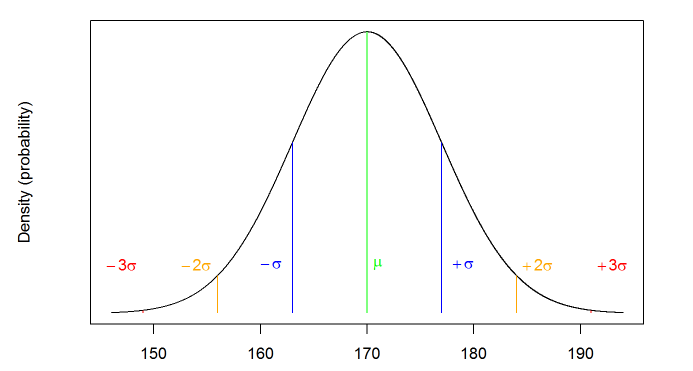
\includegraphics[width=1\linewidth,height=1\textheight]{./images/norm_dist_height} 

}

\caption{Normal Distribution of height. $\mu$ = the mean (average), $\sigma$ = standard deviation}\label{fig:unnamed-chunk-4}
\end{figure}

Normal distributions are symmetrical, meaning there is an equal probability of observations occurring above and below the mean. This means that, if the mean in figure 1 is 170, we could expect the number of people who have a height of 160 to equal the number of people who have a height of 180. This also means that the mean, median, and mode are all expected to be equal in a normal distribution.

In the same way that we could with the coin flips, we can then use what we know about our data and the normal distribution to estimate the probability of certain outcomes (e.g., what's the probability that someone would be taller than 190cm?) and we'll do this in the lab.

As with any probabilities, real-world data will come close to the normal distribution, but will (almost certainly) never match it exactly. As we collect more observations from normally-distributed data, our data will get increasingly closer to a normal distribution. As an example, here's a simulation of an experiment in which we collect heights from 5000 participants. As you can see, as we add more observations, our data starts to look more and more like the normal distribution in the previous figure.

\begin{figure}

{\centering \includegraphics[width=0.75\linewidth,height=0.75\textheight]{./images/normal_dist} 

}

\caption{A simulation of an experiment collecting height data from 2000 participants}\label{fig:unnamed-chunk-5}
\end{figure}

\hypertarget{activity-3-normal-distribution}{%
\section{Activity 3: Normal distribution}\label{activity-3-normal-distribution}}

Complete the sentences so that they are correct.

\begin{itemize}
\tightlist
\item
  In a normal distribution, the mean, median, and mode are always differentsum to zeroare all equal.
\item
  In a normal distribution, the further away from the mean an observation is the higher its probability of occuringthe lower its probability of occuring.
\item
  Whereas the binomial distribution is based on situations in which there are two possible outcomes, the normal distribution is based on situations in which the data is a continuous variablehas three possible valuesis a categorical variable.
\end{itemize}

\hypertarget{activity-4-distribution-test}{%
\section{Activity 4: Distribution test}\label{activity-4-distribution-test}}

Which distribution is likely to be associated with the following?

\begin{itemize}
\tightlist
\item
  Scores on an IQ test Uniform distributionBinomial distributionNormal distribution
\item
  Whether a country has won or lost the Eurovision song contest Uniform distributionBinomial distributionNormal distribution
\item
  Picking a spade card out of a normal pack of playing cardsUniform distributionBinomial distributionNormal distribution
\end{itemize}

In the next chapter we're going to continue looking at distributions and probability. Whilst you won't start conducting statistical tests until level 2, by the end of the next chapter you should be able to understand the core principles of probability and how we can use what we know about distributions to calculate whether a particular outcome is likely.

\hypertarget{probability-continued}{%
\chapter{Probability continued}\label{probability-continued}}

First, we're going to calculate probabilities based on the binomial distribution. In this chapter, for the first time we don't need to load the tidyverse. All the functions we need are contained in Base R. If you want a refresher on the difference between Base R and packages, see \href{https://psyteachr.github.io/ug1-practical/programming-basics.html\#packages}{Programming Basics}.

\begin{itemize}
\tightlist
\item
  Open a new R Markdown document, call it ``Probability'' and save it in your Data Skills folder.
\end{itemize}

We're going to use three Base R functions to work with the binomial distribution:

\texttt{dbinom()} - the density function: gives you the probability of x successes given the number of trials and the probability of success on a single trial (e.g., what's the probability of flipping 8/10 heads with a fair coin?).

\texttt{pbinom()} - the probability distribution function: gives you the cumulative probability of getting a number of successes below a certain cut-off point (e.g.~probability of getting 0 to 5 heads out of 10 flips), given the size and the probability. This is known as the cumulative probability distribution function or the cumulative density function.

\texttt{qbinom()} - the quantile function: is the opposite of \texttt{pbinom()} in that it gives you the x axis value for a given probability p, plus given the size and prob, that is if the probability of flipping a head is .5, how many heads would you expect to get with 10 flips?

So let's try these functions out to answer two questions:

\begin{enumerate}
\def\labelenumi{\arabic{enumi}.}
\tightlist
\item
  What is the probability of getting exactly 5 heads on 10 flips?
\item
  What is the probability of getting at most 2 heads on 10 flips?
\end{enumerate}

\hypertarget{activity-2-dbinom}{%
\section{\texorpdfstring{Activity 2: \texttt{dbinom()}}{Activity 2: dbinom()}}\label{activity-2-dbinom}}

Let's start with question 1, what is the probability of getting exactly 5 heads on 10 flips?

We want to predict the \textbf{probability} of getting 5 heads in 10 trials (coin flips) and the probability of success is 0.5 (it'll either be heads or tails so you have a 50/50 chance which we write as 0.5). We will use \texttt{dbinom()} to work this out:

The \texttt{dbinom()} (density) function has three arguments:

\begin{itemize}
\item
  \texttt{x}: the number of `heads' we want to know the probability of. Either a single one, 3 or a series 0:10. In this case it's 5.
\item
  \texttt{size}: the number of trials (flips) we are simulating; in this case, 10 flips.
\item
  \texttt{prob}: the probability of `heads' on one trial. Here chance is 50-50 which as a probability we state as 0.5 or .5
\end{itemize}

Copy, paste and run the below code in a new code chunk:

\begin{Shaded}
\begin{Highlighting}[]
\FunctionTok{dbinom}\NormalTok{(}\AttributeTok{x =} \DecValTok{5}\NormalTok{, }\AttributeTok{size =} \DecValTok{10}\NormalTok{, }\AttributeTok{prob =} \FloatTok{0.5}\NormalTok{)}
\end{Highlighting}
\end{Shaded}

\begin{itemize}
\tightlist
\item
  What is the probability of getting 5 heads out of 10 coin flips to 2 decimal places? \\
\item
  What is this probability expressed in percent? 0.25\%2.5\%25\%
\end{itemize}

\hypertarget{activity-3-pbinom}{%
\section{\texorpdfstring{Activity 3: \texttt{pbinom()}}{Activity 3: pbinom()}}\label{activity-3-pbinom}}

OK, question number 2. What is the probability of getting at most 2 heads on 10 flips?

This time we use \texttt{pbinom()} as we want to know the \textbf{cumulative probability} of getting a maximum of 2 heads from 10 coin flips. so we have set a cut-off point of 2 but we still have a probability of getting a heads of 0.5.

\textbf{Note:} \texttt{pbinom()} takes the arguments \texttt{size} and \texttt{prob} argument just like \texttt{dbinom()}. However, the first input argument is \texttt{q} rather than \texttt{x}. This is because in dbinom \texttt{x} is a fixed number, whereas \texttt{q} is all the possibilities \textbf{up to} a given number (e.g.~0, 1, 2).

Copy, paste and run the below code in a new code chunk:

\begin{Shaded}
\begin{Highlighting}[]
\FunctionTok{pbinom}\NormalTok{(}\AttributeTok{q =} \DecValTok{2}\NormalTok{, }\AttributeTok{size =} \DecValTok{10}\NormalTok{, }\AttributeTok{prob =} \FloatTok{0.5}\NormalTok{)}
\end{Highlighting}
\end{Shaded}

\begin{itemize}
\tightlist
\item
  What is the probability of getting a maximum of 2 heads on 10 coin flips to 2 decimal places? \\
\item
  What is this probability expressed in percent? 0.05\%0.5\%5\%
\end{itemize}

\hypertarget{activity-4-pbinom-2}{%
\section{\texorpdfstring{Activity 4: \texttt{pbinom()} 2}{Activity 4: pbinom() 2}}\label{activity-4-pbinom-2}}

Let's try one more scenario with a cut-off point to make sure you have understood this. What is the probability of getting 7 or more heads on 10 flips?

We can use the same function as in the previous example, however, there's an extra argument if we want to get the correct answer. Let's try running the code we used above but change \texttt{q\ =\ 2} to \texttt{q\ =\ 7}.

\begin{Shaded}
\begin{Highlighting}[]
\FunctionTok{pbinom}\NormalTok{(}\AttributeTok{q =} \DecValTok{7}\NormalTok{, }\AttributeTok{size =} \DecValTok{10}\NormalTok{, }\AttributeTok{prob =}\NormalTok{ .}\DecValTok{5}\NormalTok{) }
\end{Highlighting}
\end{Shaded}

\begin{verbatim}
## [1] 0.9453125
\end{verbatim}

This tells us that the probability is .95 or 95\% - that doesn't seem right does it? The default behaviour for \texttt{pbinom()} is to calculate cumulative probability for the lower tail of the curve, i.e., if you specify \texttt{q\ =\ 2} it calculates the probability of all outcomes below 2. We specified \texttt{q\ =\ 7} which means that it's calculated the probability of getting an outcome of 0, 1, 2, 3, 4, 5, 6, and 7, the blue area in the below figure - which is obviously very high.

\begin{figure}

{\centering \includegraphics[width=1\linewidth]{14-probability-2_files/figure-latex/unnamed-chunk-1-1} 

}

\caption{Lower and upper tails}\label{fig:unnamed-chunk-1}
\end{figure}

To get the right answer, we have to add \texttt{lower.tail\ =\ FALSE} as we are interested in the upper tail of the distribution. Because we want the cumulative probability to include 7, we set \texttt{q\ =\ 6}. This will now calculate the cumulative probability of getting 7, 8, 9, or 10 heads out of 10 coin flips.

Copy, paste and run the below code in a new code chunk:

\begin{Shaded}
\begin{Highlighting}[]
\FunctionTok{pbinom}\NormalTok{(}\AttributeTok{q =} \DecValTok{6}\NormalTok{, }\AttributeTok{size =} \DecValTok{10}\NormalTok{, }\AttributeTok{prob =}\NormalTok{ .}\DecValTok{5}\NormalTok{, }\AttributeTok{lower.tail =} \ConstantTok{FALSE}\NormalTok{) }
\end{Highlighting}
\end{Shaded}

\begin{itemize}
\tightlist
\item
  What is the probability of getting between 7 and 10 heads from 10 coin flips to 2 decimal places? \\
\item
  What is this probability expressed in percent? 0.017\%0.1717\%
\end{itemize}

\hypertarget{activity-5-qbinom}{%
\section{\texorpdfstring{Activity 5: \texttt{qbinom()}}{Activity 5: qbinom()}}\label{activity-5-qbinom}}

OK, now let's consider a scenario in which you'd use the quantile function \texttt{qbinom}. Imagine that you've been accosted by a street magician and they want to bet you that they can predict whether the coin will land on heads or tails. You suspect that they've done something to the coin so that it's not fair and that the probability of the coin landing on a head is no longer .5 or 50/50, it's now more likely to land on tails. Your null hypothesis is that the coin is not dodgy and that the probability should be even (P(heads)=.5).You are going to run a single experiment to test your hypothesis, with 10 trials. What is the minimum number of heads that is acceptable if p really does equal .5?

You have used the argument \texttt{prob} in the previous two functions, \texttt{dbinom} and \texttt{pbinom}, and it represents the probability of success on a single trial (here it is the probability of `heads' in one coin flip, .5). For \texttt{qbinom}, \texttt{prob} still represents the probability of success in one trial, whereas \texttt{p} represents the overall probability of success across all trials. When you run \texttt{pbinom}, it calculates the number of heads that would give that probability.

We know from looking at the binomial distribution above that sometimes even when the coin is fair, we won't get exactly 5/10 heads. Instead, we want to set a cut-off and in this example we will use the default cut-off for statistical significance in psychology, .05, or 5\%.

In other words, you ask it for the minimum number of successes (e.g.~heads) to maintain an overall probability of .05, in 10 flips, when the probability of a success on any one flip is .5.

\begin{Shaded}
\begin{Highlighting}[]
\FunctionTok{qbinom}\NormalTok{(}\AttributeTok{p =}\NormalTok{ .}\DecValTok{05}\NormalTok{, }\AttributeTok{size =} \DecValTok{10}\NormalTok{, }\AttributeTok{prob =}\NormalTok{ .}\DecValTok{5}\NormalTok{)}
\end{Highlighting}
\end{Shaded}

\begin{verbatim}
## [1] 2
\end{verbatim}

And it tells you the answer is 2. If the magician flipped fewer than two heads out of ten, you could conclude that there is a less than 5\% probability that would happen if the coin was fair and you would reject the null hypothesis that the coin was unbiased against heads and tell the magician to do one.

\texttt{qbinom} also uses the lower.tail argument and it works in a similar fashion to pbinom.

However, ten trials is probably far too few if you want to accuse the magician of being a bit dodge. Run the below code and then answer the following questions:

\begin{itemize}
\tightlist
\item
  What would your cut-off be if you ran 100 trials?
\item
  What would your cut-off be if you ran 1000 trials?
\item
  What would your cut-off be if you ran 10,000 trials?
\end{itemize}

\begin{Shaded}
\begin{Highlighting}[]
\FunctionTok{qbinom}\NormalTok{(}\AttributeTok{p =}\NormalTok{ .}\DecValTok{05}\NormalTok{, }\AttributeTok{size =} \FunctionTok{c}\NormalTok{(}\DecValTok{100}\NormalTok{, }\DecValTok{1000}\NormalTok{, }\DecValTok{10000}\NormalTok{), }\AttributeTok{prob =}\NormalTok{ .}\DecValTok{5}\NormalTok{)}
\end{Highlighting}
\end{Shaded}

Notice that the more trials you run, the more precise the estimates become, that is, the closer they are to the probability of success on a single flip (.5). Again this is a simplification, but think about how this relates to sample size in research studies, the more participants you have, the more precise your estimate will be.

\begin{center}\rule{0.5\linewidth}{0.5pt}\end{center}

\textbf{Visualise it!}

Have a go at playing around with different numbers of coin flips and probabilities in our \texttt{dbinom()} and \texttt{pbinom()} app!

\begin{figure}

{\centering \href{https://shannon-mcnee19.shinyapps.io/binomial_shiny/}{\includegraphics[width=1\linewidth]{14-probability-2_files/figure-latex/unnamed-chunk-2-1} }

}

\caption{Binomial distribution app}\label{fig:unnamed-chunk-2}
\end{figure}

\begin{center}\rule{0.5\linewidth}{0.5pt}\end{center}

\hypertarget{normal-distribution}{%
\section{Normal distribution}\label{normal-distribution}}

A similar set of functions exist to help us work with other distributions, including the normal distribution and we're going to use three of these:

\texttt{dnorm()}-the density function, for calculating the probability of a specific value

\texttt{pnorm()}-the probability or distribution function, for calculating the probability of getting at least or at most a specific value

\texttt{qnorm()}-the quantile function, for calculating the specific value associated with a given probability

As you can probably see, these functions are very similar to the functions we've already come across, that are used to work with the binomial distribution.

\hypertarget{probability-of-heights}{%
\section{Probability of heights}\label{probability-of-heights}}

Data from the \href{http://www.scotland.gov.uk/Resource/Doc/286063/0087158.pdf}{Scottish Health Survey (2008)} shows that:

\begin{itemize}
\tightlist
\item
  The average height of a 16-24 year old Scottish man is 176.2 centimetres, with a standard deviation of 6.748.
\item
  The average height of a 16-24 year old Scottish woman is 163.8 cm, with a standard deviation of 6.931.
\item
  There are currently no data on Scottish trans and non-binary people.
\end{itemize}

The below figure is a simulation of this data - you can see the code used to run this simulation by clicking the solution button.

Solution

\begin{Shaded}
\begin{Highlighting}[]
\NormalTok{men }\OtherTok{\textless{}{-}} \FunctionTok{rnorm}\NormalTok{(}\AttributeTok{n =} \DecValTok{100000}\NormalTok{, }\AttributeTok{mean =} \FloatTok{176.2}\NormalTok{, }\AttributeTok{sd =} \FloatTok{6.748}\NormalTok{)}
\NormalTok{women }\OtherTok{\textless{}{-}} \FunctionTok{rnorm}\NormalTok{(}\AttributeTok{n =} \DecValTok{100000}\NormalTok{, }\AttributeTok{mean =} \FloatTok{163.8}\NormalTok{, }\AttributeTok{sd =} \FloatTok{6.931}\NormalTok{)}

\NormalTok{heights }\OtherTok{\textless{}{-}} \FunctionTok{tibble}\NormalTok{(men, women) }\SpecialCharTok{\%\textgreater{}\%}
  \FunctionTok{pivot\_longer}\NormalTok{(}\AttributeTok{names\_to =} \StringTok{"sex"}\NormalTok{, }\AttributeTok{values\_to =} \StringTok{"height"}\NormalTok{, men}\SpecialCharTok{:}\NormalTok{women)}

\FunctionTok{ggplot}\NormalTok{(heights, }\FunctionTok{aes}\NormalTok{(}\AttributeTok{x =}\NormalTok{ height, }\AttributeTok{fill =}\NormalTok{ sex)) }\SpecialCharTok{+}
  \FunctionTok{geom\_density}\NormalTok{(}\AttributeTok{alpha =}\NormalTok{ .}\DecValTok{6}\NormalTok{) }\SpecialCharTok{+}
  \FunctionTok{scale\_fill\_viridis\_d}\NormalTok{(}\AttributeTok{option =} \StringTok{"E"}\NormalTok{) }\SpecialCharTok{+}
  \FunctionTok{theme\_minimal}\NormalTok{()}
\end{Highlighting}
\end{Shaded}

\begin{figure}

{\centering \includegraphics[width=1\linewidth]{14-probability-2_files/figure-latex/unnamed-chunk-4-1} 

}

\caption{Simulation of Scottish height data}\label{fig:unnamed-chunk-4}
\end{figure}

In this chapter we will use this information to calculate the probability of observing at least or at most a specific height with \texttt{pnorm()}, and the heights that are associated with specific probabilities with \texttt{qnorm()}.

\hypertarget{activity-6pnorm}{%
\section{\texorpdfstring{Activity 6:\texttt{pnorm()}}{Activity 6:pnorm()}}\label{activity-6pnorm}}

\texttt{pnorm()} requires three arguments:

\begin{itemize}
\tightlist
\item
  \texttt{q} is the value that you want to calculate the probability of
\item
  \texttt{mean} is the mean of the data
\item
  \texttt{sd} is the standard deviation of the data
\item
  \texttt{lower.tail} works as above and depends on whether you are interested in the upper or lower tail
\end{itemize}

\begin{Shaded}
\begin{Highlighting}[]
\FunctionTok{pnorm}\NormalTok{(}\AttributeTok{q =} \ConstantTok{NULL}\NormalTok{, }\AttributeTok{mean =} \ConstantTok{NULL}\NormalTok{, }\AttributeTok{sd =} \ConstantTok{NULL}\NormalTok{, }\AttributeTok{lower.tail =} \ConstantTok{NULL}\NormalTok{)}
\end{Highlighting}
\end{Shaded}

Replace the NULLs in the above code to calculate the probability of meeting a 16-24 y.o. Scottish woman who is taller than the average 16-24 y.o. Scottish man.

\begin{itemize}
\tightlist
\item
  What is the probability of meeting a 16-24 y.o. Scottish woman who is taller than the average 16-24 y.o. Scottish man? \\
\item
  What is this probability expressed in percent? 0.04\%0.4\%4\%
\end{itemize}

\hypertarget{activity-7-pnorm-2}{%
\section{\texorpdfstring{Activity 7: \texttt{pnorm} 2}{Activity 7: pnorm 2}}\label{activity-7-pnorm-2}}

Fiona is a very tall Scottish woman (181.12\nbsp{}cm) in the 16-24 y.o. range who will only date men who are taller than her.

\begin{itemize}
\tightlist
\item
  Using \texttt{pnorm()} again, what is the proportion of Scottish men Fiona would be willing to date to 2 decimal places? \\
\item
  What is this probability expressed in percent? 0.23\%2.3\%23\%
\end{itemize}

\hypertarget{activity-8-pnorm-3}{%
\section{\texorpdfstring{Activity 8: \texttt{pnorm} 3}{Activity 8: pnorm 3}}\label{activity-8-pnorm-3}}

On the other hand, Fiona will only date women who are shorter than her.

\begin{itemize}
\tightlist
\item
  What is the proportion of Scottish women would Fiona be willing to date to 2 decimal places? \\
\item
  What is this probability expressed in percent? 0.99\%9.9\%99\%
\end{itemize}

\hypertarget{activity-9-qnorm}{%
\section{\texorpdfstring{Activity 9: \texttt{qnorm()}}{Activity 9: qnorm()}}\label{activity-9-qnorm}}

In the previous examples we calculated the probability of a particular outcome. Now we want to calculate what outcome would be associated with a particular probability and we can use \texttt{qnorm()} to do this.

\texttt{qnorm()} is very similar to \texttt{pnorm()} with one exception, rather than specifying \texttt{q} our known observation or quantile, instead we have to specify \texttt{p}, our known probability.

\begin{Shaded}
\begin{Highlighting}[]
\FunctionTok{qnorm}\NormalTok{(}\AttributeTok{p =} \ConstantTok{NULL}\NormalTok{, }\AttributeTok{mean =} \ConstantTok{NULL}\NormalTok{, }\AttributeTok{sd =} \ConstantTok{NULL}\NormalTok{, }\AttributeTok{lower.tail =} \ConstantTok{NULL}\NormalTok{)}
\end{Highlighting}
\end{Shaded}

Replace the NULLs in the above code to calculate how tall a 16-24 y.o. Scottish man would have to be in order to be in the top 5\% (i.e., p = .05) of the height distribution for Scottish men in his age group.

\textbf{Visualise it!}

Have a go at playing around with different distributions in our \texttt{dnorm()} and \texttt{pnorm()} app - \href{http://shiny.psy.gla.ac.uk/jackt/ShinyPsyTeachR/ug1/normal-distributions/}{access it here}

\begin{center}\rule{0.5\linewidth}{0.5pt}\end{center}

And that's it! The key concepts to take away from this chapter are that different types of data tend to follow known distributions, and that we can use these distributions to calculate the probability of particular outcomes. This is the foundation of many of the statistical tests that you will learn about in level 2. For example, if you want to compare whether the scores from two groups are different, that is, whether they come from different distributions, you can calculate the probability that the scores from group 2 would be in the same distribution as group 1. If this probability is less than 5\% (p = .05), you might conclude that the scores were significantly different. That's an oversimplification obviously, but if you can develop a good understanding of probability distributions it will stand you in good stead for level 2.

\hypertarget{activity-solutions---probability}{%
\section{Activity solutions - Probability}\label{activity-solutions---probability}}

\hypertarget{activity-2-4}{%
\subsection{Activity 2}\label{activity-2-4}}

Solution

\begin{Shaded}
\begin{Highlighting}[]
\NormalTok{.}\DecValTok{25}
\end{Highlighting}
\end{Shaded}

\hypertarget{activity-3-5}{%
\subsection{Activity 3}\label{activity-3-5}}

Solution

\begin{Shaded}
\begin{Highlighting}[]
\NormalTok{.}\DecValTok{06}
\end{Highlighting}
\end{Shaded}

\hypertarget{activity-4-5}{%
\subsection{Activity 4}\label{activity-4-5}}

Solution

\begin{Shaded}
\begin{Highlighting}[]
\NormalTok{.}\DecValTok{17}
\end{Highlighting}
\end{Shaded}

\hypertarget{activity-5-3}{%
\subsection{Activity 5}\label{activity-5-3}}

Solution

\begin{Shaded}
\begin{Highlighting}[]
\DecValTok{42}
\DecValTok{474}
\DecValTok{4918}
\end{Highlighting}
\end{Shaded}

\hypertarget{activity-6-3}{%
\subsection{Activity 6}\label{activity-6-3}}

Solution

\begin{Shaded}
\begin{Highlighting}[]
\FunctionTok{pnorm}\NormalTok{(}\AttributeTok{q =} \FloatTok{176.2}\NormalTok{, }\AttributeTok{mean =} \FloatTok{163.8}\NormalTok{, }\AttributeTok{sd =} \FloatTok{6.931}\NormalTok{, }\AttributeTok{lower.tail =} \ConstantTok{FALSE}\NormalTok{)}
\end{Highlighting}
\end{Shaded}

\hypertarget{activity-7-1}{%
\subsection{Activity 7}\label{activity-7-1}}

Solution

\begin{Shaded}
\begin{Highlighting}[]
\FunctionTok{pnorm}\NormalTok{(}\AttributeTok{q =} \FloatTok{181.12}\NormalTok{, }\AttributeTok{mean =} \FloatTok{176.2}\NormalTok{, }\AttributeTok{sd =} \FloatTok{6.748}\NormalTok{, }\AttributeTok{lower.tail =} \ConstantTok{FALSE}\NormalTok{)}
\end{Highlighting}
\end{Shaded}

\hypertarget{activity-8-1}{%
\subsection{Activity 8}\label{activity-8-1}}

Solution

\begin{Shaded}
\begin{Highlighting}[]
\FunctionTok{pnorm}\NormalTok{(}\AttributeTok{q =} \FloatTok{181.12}\NormalTok{, }\AttributeTok{mean =} \FloatTok{163.8}\NormalTok{, }\AttributeTok{sd =} \FloatTok{6.931}\NormalTok{, }\AttributeTok{lower.tail =} \ConstantTok{TRUE}\NormalTok{)}
\end{Highlighting}
\end{Shaded}

\hypertarget{activity-9}{%
\subsection{Activity 9}\label{activity-9}}

Solution

\begin{Shaded}
\begin{Highlighting}[]
\FunctionTok{qnorm}\NormalTok{(}\AttributeTok{p =}\NormalTok{ .}\DecValTok{05}\NormalTok{, }\AttributeTok{mean =} \FloatTok{176.2}\NormalTok{, }\AttributeTok{sd =} \FloatTok{6.748}\NormalTok{, }\AttributeTok{lower.tail =} \ConstantTok{FALSE}\NormalTok{)}
\end{Highlighting}
\end{Shaded}

\hypertarget{simulation}{%
\chapter{Simulation}\label{simulation}}

Before we finish up by analysing your project data, we're going to introduce a few new functions to show you some other things that R can do and that will also reinforce your understanding of probability.

\hypertarget{simulation-1}{%
\section{Simulation}\label{simulation-1}}

One of the most powerful features of R is that you can use it for data simulation. Data simulation is the act of generating random numbers that follow a certain distribution or have known properties. This might not sound particularly impressive, but simulating data means that you can do things such as plan your statistical analyses, understand and demonstrate how probability works, or estimate how many participants you need to test in your experiment based upon what you think the data will look like. Data simulation uses the different types of distributions that we covered in Probability to generate data, so make sure that you're happy with the probability chapter before you move on.

\hypertarget{activity-1-sample}{%
\section{\texorpdfstring{Activity 1: \texttt{sample()}}{Activity 1: sample()}}\label{activity-1-sample}}

Just like Probability, all the functions we need for simulation are contained in Base R, however, we'll also load the \texttt{tidyverse} so that we can wrangle our simulated data.

Let's start by introducing the \texttt{sample()} function, which samples elements (data points) from a vector (a collection of things that are of the same type, like numbers or words). We can use \texttt{sample()} to simulate flipping a coin and build some of the graphs you saw in the probability chapter. \texttt{sample()} is used when we want to simulate discrete data, i.e., (nominal or ordinal data).

\texttt{sample()} requires you to define three arguments:

\begin{itemize}
\item
  \texttt{x} = a vector of elements, i.e., all of the possible outcomes. For our current example, this would be HEADS and TAILS.\\
\item
  \texttt{size} = how many samples do you want to take, i.e., how many times do you want R to flip the coin?\\
\item
  \texttt{replace} = specifies whether we should sample with replacement or not. In the last lab we used the example of pulling names out of a hat. If you put the name back in the hat each time you pulled one out this would be with replacement, if you don't put the name back in this would be sampling without replacement. Basically, do you want to be able to get the same outcome on different samples? For a coin flip, it should be possible to get the same outcome more than once, so we specify \texttt{TRUE}. If we specified \texttt{FALSE} you could only draw as many samples as there were unique values, so in our case we could only flip the coin twice: once it would land on heads, once on tails, and then we would run out of outcomes.
\item
  Open a new R Markdown document, name it ``Simulation'' and save it in your Data Skills folder.
\item
  Copy, paste, and run the below code in a new code chunk to simulate flipping a coin 4 times (and load the \texttt{tidyverse}).
\end{itemize}

\begin{Shaded}
\begin{Highlighting}[]
\CommentTok{\# Notice that because our event labels are strings (text), }
\CommentTok{\# we need to enter them into the function in "quotes" }
\FunctionTok{library}\NormalTok{(tidyverse)}
\FunctionTok{sample}\NormalTok{(}\AttributeTok{x =} \FunctionTok{c}\NormalTok{(}\StringTok{"HEADS"}\NormalTok{, }\StringTok{"TAILS"}\NormalTok{), }\AttributeTok{size =} \DecValTok{4}\NormalTok{, }\AttributeTok{replace =} \ConstantTok{TRUE}\NormalTok{) }
\end{Highlighting}
\end{Shaded}

\begin{verbatim}
## [1] "TAILS" "HEADS" "TAILS" "HEADS"
\end{verbatim}

How many heads did you get? Don't worry if it's different to our example. Run the code again. How many heads did you get this time? How many do you get on each turn if you run the code five more times?

When you perform data simulation, you're unlikely to get the same outcome each time you take a sample, just like if you flipped a coin 4 times on 5 separate occasions you would be unlikely to get the same number of heads each time. What's so useful about data simulation is that we can use the outcomes from lots of different sampling attempts to calculate the probability of a particular outcome, e.g., getting 4 heads from 4 flips of a coin.

So that we can add up the number of heads and tails more easily, let's simulate those coin flips again, but using numerical codes, 1 = HEADS, 0 = TAILS.

\begin{itemize}
\tightlist
\item
  Now that the outcomes are numeric, we don't need the combine function \texttt{c}\\
\item
  0:1 means all numbers from 0 to 1 in steps of 1. So basically, 0 and 1. If you wanted to simulate rolling a die, you would write \texttt{1:6} which would give you all the whole numbers from 1 to 6.
\end{itemize}

\begin{Shaded}
\begin{Highlighting}[]
\FunctionTok{sample}\NormalTok{(}\AttributeTok{x =} \DecValTok{0}\SpecialCharTok{:}\DecValTok{1}\NormalTok{, }\AttributeTok{size =} \DecValTok{4}\NormalTok{, }\AttributeTok{replace =} \ConstantTok{TRUE}\NormalTok{)}
\end{Highlighting}
\end{Shaded}

\begin{verbatim}
## [1] 0 1 1 0
\end{verbatim}

\hypertarget{activity-2-sum}{%
\section{\texorpdfstring{Activity 2: \texttt{sum()}}{Activity 2: sum()}}\label{activity-2-sum}}

Now that we're using ones and zeroes we can count the number of heads by summing the values of the outcomes. The below code will sample our coin flips as above, and then count up the outcomes. Because we've coded heads = 1 and tails = 0, we can interpret the sum of all the outcomes as the number of heads.

\begin{itemize}
\tightlist
\item
  Copy, paste and run the code below in a new code chunk.
\end{itemize}

\begin{Shaded}
\begin{Highlighting}[]
\CommentTok{\# This code pipes the output of sample() into sum() which counts up the number of heads/1s.}

\FunctionTok{sample}\NormalTok{(}\AttributeTok{x =} \DecValTok{0}\SpecialCharTok{:}\DecValTok{1}\NormalTok{, }\AttributeTok{size =} \DecValTok{4}\NormalTok{, }\AttributeTok{replace =} \ConstantTok{TRUE}\NormalTok{) }\SpecialCharTok{\%\textgreater{}\%} \FunctionTok{sum}\NormalTok{()}
\end{Highlighting}
\end{Shaded}

\begin{verbatim}
## [1] 1
\end{verbatim}

Run this function multiple times (you can use the green markdown play arrow at the top right of the code chunk to make this easy). In our simulation of five sets of four flips we got 1, 3, 2, 2, and 3 heads. So in only one out of the five simulations did we get exactly one heads, i.e., a proportion of .2 or 20\% of the time.

\hypertarget{activity-3-replicate-1}{%
\section{\texorpdfstring{Activity 3: \texttt{replicate()} 1}{Activity 3: replicate() 1}}\label{activity-3-replicate-1}}

Let's repeat the experiment a whole bunch more times. We can have R do this over and over again using the \texttt{replicate()} function. \texttt{replicate()} requires two arguments (although there are other optional arguments if you want to do more complicated tasks):

\begin{itemize}
\tightlist
\item
  \texttt{n} = the number of times you want to repeat your code\\
\item
  \texttt{expr} = the expression, or code, you want to repeat
\end{itemize}

Copy, paste and run the below code into a new code chunk to run the sample function and sum up the outcomes 20 times.

\begin{Shaded}
\begin{Highlighting}[]
\FunctionTok{replicate}\NormalTok{(}\AttributeTok{n =} \DecValTok{20}\NormalTok{, }\AttributeTok{expr =} \FunctionTok{sample}\NormalTok{(}\DecValTok{0}\SpecialCharTok{:}\DecValTok{1}\NormalTok{, }\DecValTok{4}\NormalTok{, }\ConstantTok{TRUE}\NormalTok{) }\SpecialCharTok{\%\textgreater{}\%} \FunctionTok{sum}\NormalTok{())}
\end{Highlighting}
\end{Shaded}

\begin{verbatim}
##  [1] 3 3 2 1 2 3 1 2 3 2 2 4 2 3 3 2 2 3 1 1
\end{verbatim}

\hypertarget{monte-carlo-simulation}{%
\section{Monte Carlo simulation}\label{monte-carlo-simulation}}

Every year, the city of Monte Carlo is the site of innumerable games of chance played in its casinos by people from all over the world. This notoriety is reflected in the use of the term ``Monte Carlo simulation'' among statisticians to refer to using a computer simulation to estimate statistical properties of a random process. In a Monte Carlo simulations, the random process is repeated over and over again in order to assess its performance over a very large number of trials. It is usually used in situations where mathematical solutions are unknown or hard to compute. Now we are ready to use Monte Carlo simulation to demonstrate the probability of various outcomes.

\hypertarget{activity-4-replicate-2}{%
\section{\texorpdfstring{Activity 4: \texttt{replicate()} 2}{Activity 4: replicate() 2}}\label{activity-4-replicate-2}}

We are going to run our coin flip experiment again but this time we are going to run the experiment 50 times (each including 4 coin tosses), and use the same principles to predict the number of heads we will get.

\begin{itemize}
\tightlist
\item
  Copy, paste, and run the below code to run the simulation and store the result in an object `heads50** using the code below:
\end{itemize}

\begin{Shaded}
\begin{Highlighting}[]
\NormalTok{heads50 }\OtherTok{\textless{}{-}} \FunctionTok{replicate}\NormalTok{(}\DecValTok{50}\NormalTok{, }\FunctionTok{sample}\NormalTok{(}\DecValTok{0}\SpecialCharTok{:}\DecValTok{1}\NormalTok{, }\DecValTok{4}\NormalTok{, }\ConstantTok{TRUE}\NormalTok{) }\SpecialCharTok{\%\textgreater{}\%} \FunctionTok{sum}\NormalTok{())   }
\NormalTok{heads50}
\end{Highlighting}
\end{Shaded}

\begin{verbatim}
##  [1] 3 3 2 3 2 2 1 1 2 2 3 3 1 2 1 0 3 3 1 1 1 1 2 3 2 3 1 3 2 0 4 3 2 3 1 1 2 3
## [39] 2 2 0 1 1 2 2 1 3 3 2 2
\end{verbatim}

\hypertarget{activity-5-probability}{%
\section{Activity 5: probability}\label{activity-5-probability}}

We can estimate the probability of each of the outcomes (0, 1, 2, 3, 4 heads after 4 coin tosses) by counting them up and dividing by the number of experiments. We will do this by putting the results of the replications in a tibble() and then using count().

\begin{Shaded}
\begin{Highlighting}[]
\NormalTok{data50 }\OtherTok{\textless{}{-}} \FunctionTok{tibble}\NormalTok{(}\AttributeTok{heads =}\NormalTok{ heads50) }\SpecialCharTok{\%\textgreater{}\%}   \CommentTok{\# convert to a table}
                \FunctionTok{group\_by}\NormalTok{(heads) }\SpecialCharTok{\%\textgreater{}\%}   \CommentTok{\# group by number of possibilities (0,1,2,3,4)}
                \FunctionTok{summarise}\NormalTok{(}\AttributeTok{n =} \FunctionTok{n}\NormalTok{(), }\CommentTok{\# count occurances of each possibility,}
                          \AttributeTok{p=}\NormalTok{n}\SpecialCharTok{/}\DecValTok{50}\NormalTok{) }\CommentTok{\# \& calculate probability (p) of each}
\end{Highlighting}
\end{Shaded}

\begin{tabular}{r|r|r}
\hline
heads & n & p\\
\hline
0 & 3 & 0.06\\
\hline
1 & 14 & 0.28\\
\hline
2 & 17 & 0.34\\
\hline
3 & 15 & 0.30\\
\hline
4 & 1 & 0.02\\
\hline
\end{tabular}

Your numbers may be slightly different to the ones presented in this book - remember that by default, each time you run a simulation, you will get a different random sample.

\hypertarget{activity-6-visualisation}{%
\section{Activity 6: visualisation}\label{activity-6-visualisation}}

We can then plot a histogram of the outcomes using \texttt{geom\_bar()}.

\begin{Shaded}
\begin{Highlighting}[]
\CommentTok{\# Note: stat = "identity" tells  ggplot to use the values of the y{-}axis variable (p) as the height of the bars in our histogram (as opposed to counting the number of occurances of those values)}

\FunctionTok{ggplot}\NormalTok{(data50, }\FunctionTok{aes}\NormalTok{(}\AttributeTok{x =}\NormalTok{ heads,}\AttributeTok{y =}\NormalTok{ p)) }\SpecialCharTok{+} 
  \FunctionTok{geom\_bar}\NormalTok{(}\AttributeTok{stat =} \StringTok{"identity"}\NormalTok{, }\AttributeTok{fill =} \StringTok{"purple"}\NormalTok{) }\SpecialCharTok{+} 
  \FunctionTok{labs}\NormalTok{(}\AttributeTok{x =} \StringTok{"Number of Heads"}\NormalTok{, }\AttributeTok{y =} \StringTok{"Probability of Heads in 4 flips (p)"}\NormalTok{) }\SpecialCharTok{+}
  \FunctionTok{theme\_minimal}\NormalTok{()}
\end{Highlighting}
\end{Shaded}

\begin{figure}

{\centering 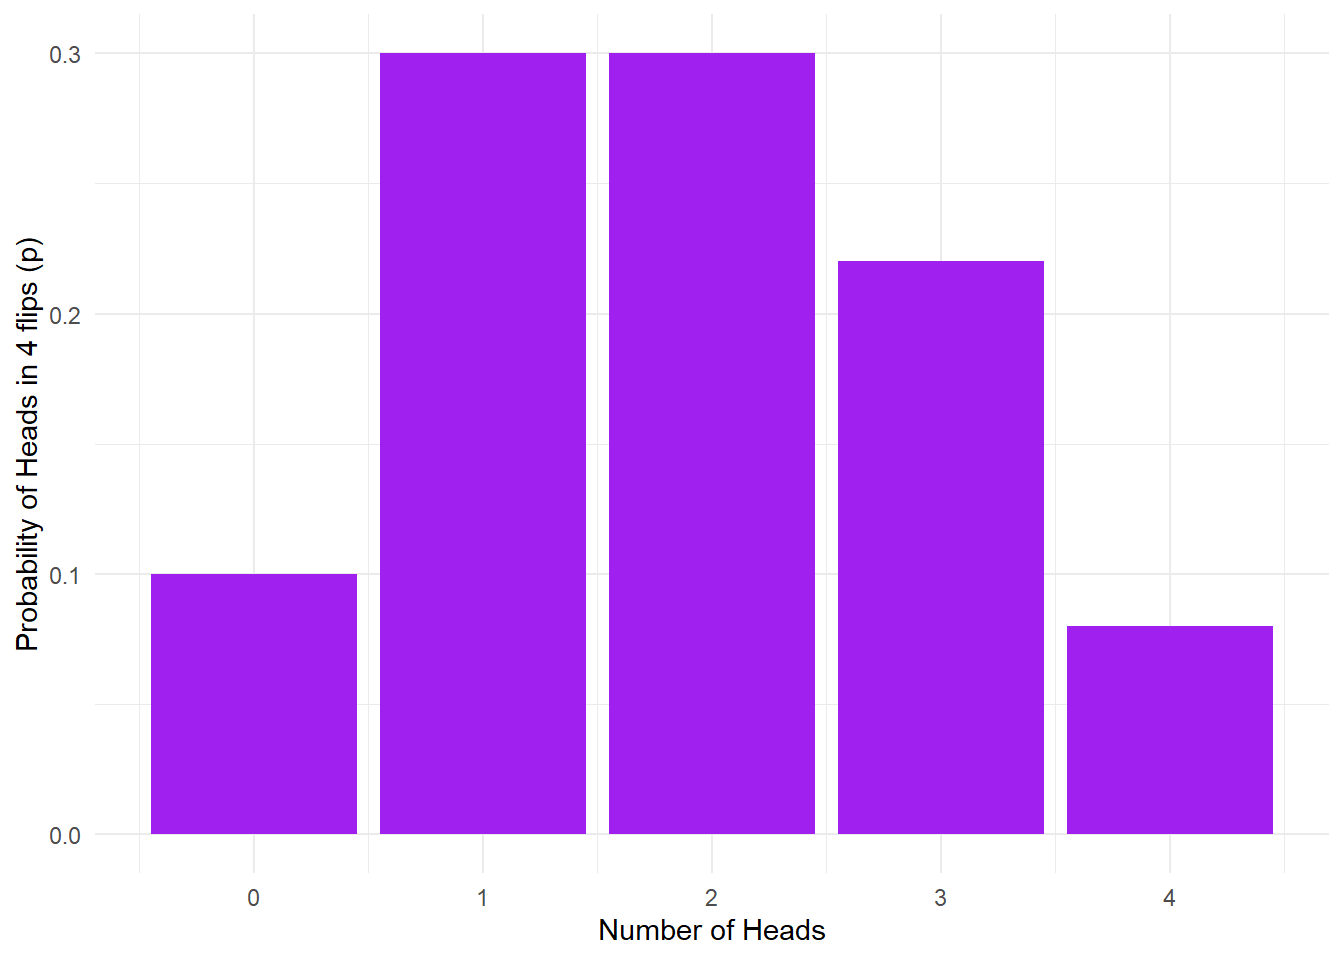
\includegraphics[width=1\linewidth]{15-simulation_files/figure-latex/data50hist-1} 

}

\caption{No. of heads from 4 coin tosses probability outcomes.}\label{fig:data50hist}
\end{figure}

\begin{center}\rule{0.5\linewidth}{0.5pt}\end{center}

\textbf{Pause here and interpret the above figure}

\begin{itemize}
\tightlist
\item
  What is the estimated probability for flipping 0/4 heads? 1/4 heads? 2/4 heads? 3/4 heads? 4/4 heads?
\end{itemize}

\begin{center}\rule{0.5\linewidth}{0.5pt}\end{center}

Unfortunately sometimes this calculation will estimate that the probability of an outcome is zero since this outcome never came up when the simulation is run. If you want reliable estimates, you need a \textbf{bigger sample} to minimise the probability that a possible outcome won't occur.

\hypertarget{activity-7-big-data}{%
\section{Activity 7: big data}\label{activity-7-big-data}}

Let's repeat the Monte Carlo simulation, but with 10,000 trials instead of just 50. All we need to do is change \texttt{n} from 50 to 10000.

\begin{Shaded}
\begin{Highlighting}[]
\NormalTok{heads10K }\OtherTok{\textless{}{-}} \FunctionTok{replicate}\NormalTok{(}\AttributeTok{n =} \DecValTok{10000}\NormalTok{, }\AttributeTok{expr =} \FunctionTok{sample}\NormalTok{(}\DecValTok{0}\SpecialCharTok{:}\DecValTok{1}\NormalTok{, }\DecValTok{4}\NormalTok{, }\ConstantTok{TRUE}\NormalTok{) }\SpecialCharTok{\%\textgreater{}\%} \FunctionTok{sum}\NormalTok{())   }
\end{Highlighting}
\end{Shaded}

Again, we'll put the outcome into a table using \texttt{tibble} and calculate counts and probabilities of each outcome using \texttt{group\_by()} and \texttt{summarise()}. Remember to try reading your code in full sentences to help you understand what multiple lines of code connected by pipes are doing. How would you read the below code?

\begin{Shaded}
\begin{Highlighting}[]
\NormalTok{data10K }\OtherTok{\textless{}{-}} \FunctionTok{tibble}\NormalTok{(}\AttributeTok{heads =}\NormalTok{ heads10K) }\SpecialCharTok{\%\textgreater{}\%}   
                \FunctionTok{group\_by}\NormalTok{(heads) }\SpecialCharTok{\%\textgreater{}\%}           
                \FunctionTok{summarise}\NormalTok{(}\AttributeTok{n =} \FunctionTok{n}\NormalTok{(), }\AttributeTok{p=}\NormalTok{n}\SpecialCharTok{/}\DecValTok{10000}\NormalTok{) }
\end{Highlighting}
\end{Shaded}

Finally, we can visualise this as we did earlier.

\begin{Shaded}
\begin{Highlighting}[]
\FunctionTok{ggplot}\NormalTok{(data10K, }\FunctionTok{aes}\NormalTok{(heads,p)) }\SpecialCharTok{+} 
  \FunctionTok{geom\_bar}\NormalTok{(}\AttributeTok{stat =} \StringTok{"identity"}\NormalTok{, }\AttributeTok{fill =} \StringTok{"purple"}\NormalTok{) }\SpecialCharTok{+} 
  \FunctionTok{labs}\NormalTok{(}\AttributeTok{x =} \StringTok{"Number of Heads"}\NormalTok{, }\AttributeTok{y =} \StringTok{"Probability of Heads in 4 flips (p)"}\NormalTok{) }\SpecialCharTok{+}
  \FunctionTok{theme\_minimal}\NormalTok{()}
\end{Highlighting}
\end{Shaded}

\begin{figure}

{\centering 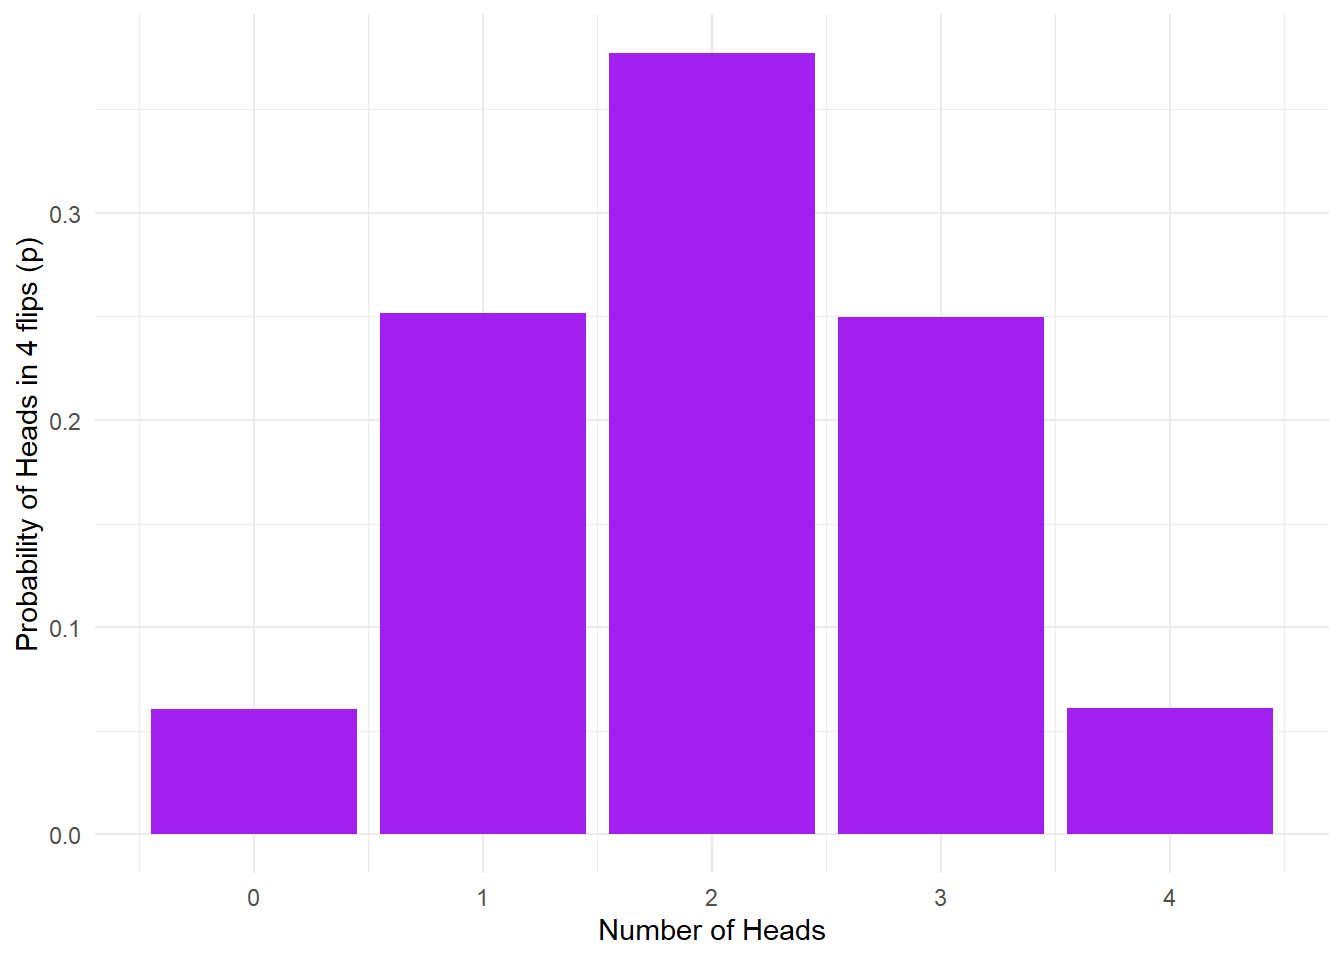
\includegraphics[width=1\linewidth]{15-simulation_files/figure-latex/data10Khist-1} 

}

\caption{10K coin toss probability outcomes.}\label{fig:data10Khist}
\end{figure}

Using Monte Carlo simulation, we estimate that the probability of getting exactly one head on four throws is about 0.25. The above result represents a probability distribution for all the possible outcomes in our experiments. We can derive lots of useful information from this.

For instance, what is the probability of getting two or more heads in four throws? This is easy: the outcomes meeting the criterion are 2, 3, or 4 heads. We can just add these probabilities together like so:

\begin{Shaded}
\begin{Highlighting}[]
\NormalTok{data10K }\SpecialCharTok{\%\textgreater{}\%}
  \FunctionTok{filter}\NormalTok{(heads }\SpecialCharTok{\textgreater{}=} \DecValTok{2}\NormalTok{) }\SpecialCharTok{\%\textgreater{}\%}
  \FunctionTok{summarise}\NormalTok{(}\AttributeTok{p2 =} \FunctionTok{sum}\NormalTok{(p))}
\end{Highlighting}
\end{Shaded}

\begin{verbatim}
## # A tibble: 1 x 1
##      p2
##   <dbl>
## 1 0.689
\end{verbatim}

You can add probabilities for various outcomes together as long as the outcomes are mutually exclusive, that is, when one outcome occurs, the others can't occur. For this coin flipping example, this is obviously the case: you can't simultaneously get exactly two and exactly three heads as the outcome of a single experiment. However, be aware that you can't simply add probabilities together when the events in question are not mutually exclusive: for example, the probability of the coin landing heads up, and it landing with the image of the head being in a particular orientation are not mutually exclusive, and can't be simply added together.

This is the basis of how we can calculate the probability of an outcome using a known distribution - by simulating a large number of trials we can use this as an estimate for how our data will look in the real world.

\hypertarget{activity-8-rnorm}{%
\section{\texorpdfstring{Activity 8: \texttt{rnorm()}}{Activity 8: rnorm()}}\label{activity-8-rnorm}}

We can also use R to simulate continuous data that follow a normal distribution using \texttt{rnorm()}. You've actually used \texttt{rnorm()} before, all the way back in Intro to R from Psych 1A but we'll go over it again.

\begin{itemize}
\tightlist
\item
  \texttt{n} is the number of data points you wish to simulate which is the only required argument for \texttt{rnorm()}
\item
  \texttt{mean} is the mean that you want your data to have. If you don't provide this argument, \texttt{rnorm()} will use a default value of \texttt{mean\ =\ 0}.
\item
  \texttt{sd} is the standard deviation you want your data to have. If you don't provide this argument, \texttt{rnorm()} will use a default value of \texttt{sd\ =\ 1}.
\end{itemize}

Copy, paste and run the below code in a new code chunk. This will randomly generate 50 numbers that collectively have a mean of 10 and a SD of 2 and then store it in the object \texttt{normal}.

\begin{Shaded}
\begin{Highlighting}[]
\NormalTok{normal }\OtherTok{\textless{}{-}} \FunctionTok{rnorm}\NormalTok{(}\AttributeTok{n =} \DecValTok{50}\NormalTok{, }\AttributeTok{mean =} \DecValTok{10}\NormalTok{, }\AttributeTok{sd =} \DecValTok{2}\NormalTok{)}
\end{Highlighting}
\end{Shaded}

You can check that the data you have generated are as you expected by calculating the mean and SD of this new variable - you shouldn't expect the values to be exactly 10 and 2 (remember, it's randomly generated), but they should be reasonably close.

\begin{Shaded}
\begin{Highlighting}[]
\FunctionTok{mean}\NormalTok{(normal)}
\FunctionTok{sd}\NormalTok{(normal)}
\end{Highlighting}
\end{Shaded}

\begin{verbatim}
## [1] 9.9299
## [1] 2.256631
\end{verbatim}

Finally, you can visualise your data with a density plot. Try changing the number of data points generated by \texttt{rnorm()} from 50 to 500 to 5000 and then see how the shape of the distribution changes.

\begin{Shaded}
\begin{Highlighting}[]
\FunctionTok{tibble}\NormalTok{(}\AttributeTok{normal =}\NormalTok{ normal) }\SpecialCharTok{\%\textgreater{}\%} \CommentTok{\#turn the variable normal into a table and then}
  \FunctionTok{ggplot}\NormalTok{(}\FunctionTok{aes}\NormalTok{(normal)) }\SpecialCharTok{+} \CommentTok{\# create a density plot}
  \FunctionTok{geom\_density}\NormalTok{(}\AttributeTok{fill =} \StringTok{"red"}\NormalTok{) }\SpecialCharTok{+}
  \FunctionTok{theme\_minimal}\NormalTok{()}
\end{Highlighting}
\end{Shaded}

\begin{figure}

{\centering \includegraphics[width=1\linewidth]{15-simulation_files/figure-latex/unnamed-chunk-3-1} 

}

\caption{Distribution of variable created by rnorm}\label{fig:unnamed-chunk-3}
\end{figure}

\hypertarget{activity-9-simulate-a-dataset}{%
\section{Activity 9: Simulate a dataset}\label{activity-9-simulate-a-dataset}}

Finally, we can put all of this together to simulate a full dataset. Let's imagine that we're going to run an experiment to see whether 120 people will roll a higher number on a die if their IQ is higher. This is obviously a stupid experiment but psychology does occasionally do stupid things.

\begin{itemize}
\tightlist
\item
  First, let's create a variable that has all of our subject IDs. We're just going to assign our participants numerical codes.
\end{itemize}

\begin{Shaded}
\begin{Highlighting}[]
\NormalTok{subject\_id }\OtherTok{\textless{}{-}} \DecValTok{1}\SpecialCharTok{:}\DecValTok{120} \CommentTok{\# create a variable called subject\_id that has the numbers 1 to 120 in it}
\end{Highlighting}
\end{Shaded}

Then we're going to create a column for gender using a new but simple function \texttt{rep} which stands for ``repeat''. The below code will create a variable that repeats ``man'' 40 times, then ``women'' 40 times, then ``non-binary'' 40 times.

\begin{Shaded}
\begin{Highlighting}[]
\NormalTok{gender }\OtherTok{\textless{}{-}} \FunctionTok{rep}\NormalTok{(}\AttributeTok{x =} \FunctionTok{c}\NormalTok{(}\StringTok{"man"}\NormalTok{, }\StringTok{"woman"}\NormalTok{, }\StringTok{"nonbinary"}\NormalTok{), }\AttributeTok{each =} \DecValTok{40}\NormalTok{)}
\end{Highlighting}
\end{Shaded}

Next, let's simulate them all rolling a die once using \texttt{sample()}.

\begin{Shaded}
\begin{Highlighting}[]
\NormalTok{rolls }\OtherTok{\textless{}{-}} \FunctionTok{sample}\NormalTok{(}\AttributeTok{x =} \DecValTok{1}\SpecialCharTok{:}\DecValTok{6}\NormalTok{, }\AttributeTok{size =} \DecValTok{120}\NormalTok{, }\AttributeTok{replace =} \ConstantTok{TRUE}\NormalTok{)}
\end{Highlighting}
\end{Shaded}

Then, let's simulate their IQ scores. IQ scores are standardised so that overall, the population has an average IQ of 100 and a SD of 15 so we can use this information to simulate the data with \texttt{rnorm()}.

\begin{Shaded}
\begin{Highlighting}[]
\NormalTok{iq }\OtherTok{\textless{}{-}} \FunctionTok{rnorm}\NormalTok{(}\AttributeTok{n =} \DecValTok{120}\NormalTok{, }\AttributeTok{mean =} \DecValTok{100}\NormalTok{, }\AttributeTok{sd =} \DecValTok{15}\NormalTok{)}
\end{Highlighting}
\end{Shaded}

Finally, we can stitch all these variables together into a table.

\begin{Shaded}
\begin{Highlighting}[]
\NormalTok{sim\_data }\OtherTok{\textless{}{-}} \FunctionTok{tibble}\NormalTok{(subject\_id, gender, rolls, iq)}
\end{Highlighting}
\end{Shaded}

Now that we've got our simulated data we could write code to analyse it even before we've collected any real data which will not only save us time in the future, but will help us plan our analyses and we could include this code in a pre-registration document.

For example, you could create a plot of IQ scores for each dice roll (remember these are not real data\ldots)

\begin{Shaded}
\begin{Highlighting}[]
\NormalTok{sim\_data }\SpecialCharTok{\%\textgreater{}\%}
  \FunctionTok{mutate}\NormalTok{(}\AttributeTok{rolls =} \FunctionTok{as.factor}\NormalTok{(rolls)) }\SpecialCharTok{\%\textgreater{}\%}
  \FunctionTok{ggplot}\NormalTok{(}\FunctionTok{aes}\NormalTok{(}\AttributeTok{x =}\NormalTok{ rolls, }\AttributeTok{y =}\NormalTok{ iq, }\AttributeTok{fill =}\NormalTok{ rolls)) }\SpecialCharTok{+}
  \FunctionTok{geom\_violin}\NormalTok{(}\AttributeTok{trim =} \ConstantTok{FALSE}\NormalTok{, }\AttributeTok{alpha =}\NormalTok{ .}\DecValTok{6}\NormalTok{, }\AttributeTok{show.legend =} \ConstantTok{FALSE}\NormalTok{) }\SpecialCharTok{+}
  \FunctionTok{geom\_boxplot}\NormalTok{(}\AttributeTok{width =}\NormalTok{ .}\DecValTok{2}\NormalTok{, }\AttributeTok{show.legend =} \ConstantTok{FALSE}\NormalTok{) }\SpecialCharTok{+}
  \FunctionTok{scale\_fill\_viridis\_d}\NormalTok{(}\AttributeTok{option =} \StringTok{"E"}\NormalTok{) }\SpecialCharTok{+}
  \FunctionTok{theme\_minimal}\NormalTok{() }\SpecialCharTok{+}
  \FunctionTok{labs}\NormalTok{(}\AttributeTok{x =} \StringTok{"Outcome of dice roll"}\NormalTok{)}
\end{Highlighting}
\end{Shaded}

\begin{figure}

{\centering \includegraphics[width=1\linewidth]{15-simulation_files/figure-latex/unnamed-chunk-9-1} 

}

\caption{Boxplot of IQ scores grouped by what each person rolled on the die}\label{fig:unnamed-chunk-9}
\end{figure}

\hypertarget{finished-6}{%
\section{Finished!}\label{finished-6}}

The final Data Skills activity is to analyse your group project data which means in terms of new stuff to learn, we're done! In Psych 1A and 1B, we've tried to give you a solid introduction to common data skills you'll need in order to conduct your own research. Even if you don't intend to continue with psychology or quantitative research in the future, we hope that you're proud of the skills you've learned. For some of you, R might not have been your favourite bit of the course, but you should be very proud of what you've achieved and with such a diverse class we hope you can see that programming isn't an innate skill that only certain people can learn. It just take a a bit of work, some (hopefully) helpful teaching materials, and a lot of swearing at the error messages.

\hypertarget{project-analysis}{%
\chapter{Project analysis}\label{project-analysis}}

We've spent the last 6 months giving you the skills you need to be able to deal with your own data. Now's the time to show us what you've learned. In this chapter we're going to describe the steps you will need to go through when analysing your data but, aside from a few lines that will help you deal with the questionnaire data that the Experimentum platform spits out, we're not going to give you any code solutions.

Everything you need to do you've done before, so use this book to help you. Remember, you don't need to write the code from memory, you just need to find the relevant examples and then copy and paste and change what needs changing to make it work for you.

We suggest that you problem-solve the code as a group, however, make sure that you all have a separate copy of the final working code. You can book into GTA sessions in week 9 and 10 to help you as well.

\hypertarget{step-1-load-in-packages-and-data}{%
\section{Step 1: Load in packages and data}\label{step-1-load-in-packages-and-data}}

The data file \texttt{final\_data.csv} is on Moodle in the Group Poster section.

Don't change ANY of the code from step 1. Just copy and paste it into R EXACTLY as it is below.

This code will clean up the Experimentum data a little bit to help you on your way. You will get a message saying \texttt{NAs\ introduced\ by\ coercion}. Ignore this message, it's a result of converting the employment hours to a numeric variable.

It's also worth noting that this is a MUCH larger dataset than any you've worked with so far and you might find that R takes a little longer to complete each task - this is perfectly normal.

\begin{Shaded}
\begin{Highlighting}[]
\FunctionTok{library}\NormalTok{(tidyverse)}

\NormalTok{dat }\OtherTok{\textless{}{-}} \FunctionTok{read\_csv}\NormalTok{(}\StringTok{"final\_data.csv"}\NormalTok{, }
                \AttributeTok{col\_types =} \FunctionTok{cols}\NormalTok{(}\AttributeTok{team =} \FunctionTok{col\_factor}\NormalTok{(), }
                                 \AttributeTok{dv =} \FunctionTok{col\_character}\NormalTok{()))}

\NormalTok{demo }\OtherTok{\textless{}{-}}\NormalTok{  dat }\SpecialCharTok{\%\textgreater{}\%}
  \FunctionTok{filter}\NormalTok{(quest\_id }\SpecialCharTok{==} \StringTok{"1448"}\NormalTok{) }\SpecialCharTok{\%\textgreater{}\%}
  \FunctionTok{select}\NormalTok{(user\_id, user\_sex, user\_age, q\_name, dv, covid) }\SpecialCharTok{\%\textgreater{}\%}
  \FunctionTok{pivot\_wider}\NormalTok{(}\AttributeTok{names\_from =} \StringTok{"q\_name"}\NormalTok{, }\AttributeTok{values\_from =} \StringTok{"dv"}\NormalTok{) }\SpecialCharTok{\%\textgreater{}\%}
  \FunctionTok{select}\NormalTok{(}\SpecialCharTok{{-}}\StringTok{"NA"}\NormalTok{) }\SpecialCharTok{\%\textgreater{}\%}
  \FunctionTok{mutate}\NormalTok{(}\AttributeTok{employment =} \FunctionTok{as.numeric}\NormalTok{(employment))}

\NormalTok{teams }\OtherTok{\textless{}{-}}\NormalTok{  dat }\SpecialCharTok{\%\textgreater{}\%}
  \FunctionTok{filter}\NormalTok{(q\_name }\SpecialCharTok{==} \StringTok{"team\_name"}\NormalTok{) }\SpecialCharTok{\%\textgreater{}\%}
  \FunctionTok{select}\NormalTok{(user\_id, team)}

\NormalTok{mslq }\OtherTok{\textless{}{-}}\NormalTok{  dat }\SpecialCharTok{\%\textgreater{}\%}
  \FunctionTok{filter}\NormalTok{(quest\_id }\SpecialCharTok{==} \StringTok{"1449"}\NormalTok{) }\SpecialCharTok{\%\textgreater{}\%}
  \FunctionTok{select}\NormalTok{(user\_id, q\_name, dv) }\SpecialCharTok{\%\textgreater{}\%}
  \FunctionTok{mutate}\NormalTok{(}\AttributeTok{dv =} \FunctionTok{as.numeric}\NormalTok{(dv)) }\SpecialCharTok{\%\textgreater{}\%}
  \FunctionTok{arrange}\NormalTok{(q\_name) }\SpecialCharTok{\%\textgreater{}\%}
  \FunctionTok{pivot\_wider}\NormalTok{(}\AttributeTok{names\_from =} \StringTok{"q\_name"}\NormalTok{, }\AttributeTok{values\_from =} \StringTok{"dv"}\NormalTok{)}

\NormalTok{final\_dat }\OtherTok{\textless{}{-}} \FunctionTok{left\_join}\NormalTok{(demo, teams) }\SpecialCharTok{\%\textgreater{}\%}
  \FunctionTok{inner\_join}\NormalTok{(mslq)}
\end{Highlighting}
\end{Shaded}

Right. Your turn. You may find it helpful to use the search function in this book to find examples of the code you need.

\begin{figure}

{\centering \includegraphics[width=0.75\linewidth,height=0.75\textheight]{./images/searching} 

}

\caption{Searching for functions}\label{fig:unnamed-chunk-2}
\end{figure}

\hypertarget{step-2-look-at-the-data}{%
\section{Step 2: Look at the data}\label{step-2-look-at-the-data}}

\texttt{final\_dat} should have 91 columns which means that R won't show you them all if you just click on the object, you'll need to run \texttt{summary()}. Have a look at what all the variables are, you will find it helpful to refer to the Survey Variables Overview document.

\hypertarget{step-3.-select-your-variables}{%
\section{Step 3. Select your variables}\label{step-3.-select-your-variables}}

Use \texttt{select()} to retain only the variables you need for your chosen research design and analysis, i.e.~the responses to the sub-scale you're interested in as well as the user id, sex, age, team number, and any variables you're going to use as criteria for inclusion. Again, you might find it helpful to consult the survey variables overview document to get the variable names.

\hypertarget{step-4-factors}{%
\section{Step 4: Factors}\label{step-4-factors}}

Using \texttt{summary()} again if you need it, check what type of variable each column is. Recode any variables that you want to use as categorical variables as factors and then run summary again to see how many you have in each group. You will find the code book you downloaded with the data files from Moodle helpful for this task. You may find the \href{https://psyteachr.github.io/ug1-practical/intro-to-data-viz.html\#activity-3-factors}{Data Visualisation activity about factors} helpful for this.

\hypertarget{step-5-filter}{%
\section{Step 5: Filter}\label{step-5-filter}}

If necessary, use \texttt{filter()} to retain only the observations you need, for example, you might need to delete participants above a certain age, or only use mature students or undergraduate students (and make sure you kept all these columns in step 3). Do not filter the data for your team yet. You will find the code book you downloaded with the data files from Moodle helpful for this task.

If your grouping variable is whether students undertake paid employment, you will need to create a new variable using mutate that categorises participants into employed (\textgreater{} 0 hours worked per week) and not employed (0 hours per week) categories.

An additional bit of syntax you might find useful for this is the \texttt{\%in\%} notation which allows you to filter by multiple values. For example, the following code will retain all rows where \texttt{user\_sex} equals male OR female and nothing else (i.e., it would get rid of non-binary participants, prefer not to says, and missing values).

\begin{Shaded}
\begin{Highlighting}[]
\NormalTok{dat }\SpecialCharTok{\%\textgreater{}\%}
  \FunctionTok{filter}\NormalTok{(user\_sex }\SpecialCharTok{\%in\%} \FunctionTok{c}\NormalTok{(}\StringTok{"male"}\NormalTok{, }\StringTok{"female"}\NormalTok{))}
\end{Highlighting}
\end{Shaded}

You can also do it by exclusion with \texttt{!}. The below code would retain everything where \texttt{user\_sex} DOESN'T equal male or female.

\begin{Shaded}
\begin{Highlighting}[]
\NormalTok{dat }\SpecialCharTok{\%\textgreater{}\%}
  \FunctionTok{filter}\NormalTok{(}\SpecialCharTok{!}\NormalTok{user\_sex }\SpecialCharTok{\%in\%} \FunctionTok{c}\NormalTok{(}\StringTok{"male"}\NormalTok{, }\StringTok{"female"}\NormalTok{))}
\end{Highlighting}
\end{Shaded}

If you were feeling really fancy you could do steps 2 - 5 in a single pipeline of code.

\hypertarget{step-6-sub-scale-scores}{%
\section{Step 6: Sub-scale scores}\label{step-6-sub-scale-scores}}

Calculate the mean score for each participant for your chosen sub-scale. There are a few ways you can do this but helpfully the \href{https://gla-my.sharepoint.com/:w:/g/personal/2087153l_student_gla_ac_uk/EfFPtssPMV9HkrZALfdln8wBBJKClQ0eAXzrrHxa0nOo7g?e=SNIhSt}{Experimentum documentation} provides example code to make this easier, you just need to adapt it for the variables you need. You may also want to change the \texttt{na.rm\ =\ TRUE} for the calculation of means depending on whether you want to only include participants who completed all questions.

\begin{itemize}
\tightlist
\item
  Change \texttt{data} to the name of the object you created in step 6
\item
  Change \texttt{question\_1:question\_5} to the relevant variables for your subscale e.g., \texttt{help\_1:help\_4}
\item
  Change \texttt{scale\_mean} to the name of your sub-scale e.g., \texttt{anxiety\_mean}
\item
  If you want to calculate the mean scores for participants who have missing data, e.g., if they only completed three out of four questions for your sub-scale, then \texttt{na.rm\ =\ TRUE}. If you only want to calculate scores for participants who answered all questions for your sub-scale, then \texttt{na.rm\ =\ FALSE}.
\item
  Change NOTHING else
\end{itemize}

You may get the message \texttt{summarise()\ regrouping\ output\ by....} this is fine.

\begin{Shaded}
\begin{Highlighting}[]
\NormalTok{dat\_means }\OtherTok{\textless{}{-}}\NormalTok{ data }\SpecialCharTok{\%\textgreater{}\%} 
  \FunctionTok{pivot\_longer}\NormalTok{(}\AttributeTok{names\_to =} \StringTok{"var"}\NormalTok{, }\AttributeTok{values\_to =} \StringTok{"val"}\NormalTok{, question\_1}\SpecialCharTok{:}\NormalTok{question\_5) }\SpecialCharTok{\%\textgreater{}\%} 
  \FunctionTok{group\_by\_at}\NormalTok{(}\FunctionTok{vars}\NormalTok{(}\SpecialCharTok{{-}}\NormalTok{val, }\SpecialCharTok{{-}}\NormalTok{var)) }\SpecialCharTok{\%\textgreater{}\%} 
  \FunctionTok{summarise}\NormalTok{(}\AttributeTok{scale\_mean =} \FunctionTok{mean}\NormalTok{(val, }\AttributeTok{na.rm =} \ConstantTok{TRUE}\NormalTok{)) }\SpecialCharTok{\%\textgreater{}\%} 
  \FunctionTok{ungroup}\NormalTok{() }
\end{Highlighting}
\end{Shaded}

Optional: If you want a dataset that just has complete cases, then you can run the below code. This will remove any participants who have an \texttt{NA} for scale-score due to missing data.

\begin{Shaded}
\begin{Highlighting}[]
\NormalTok{dat\_means\_complete }\OtherTok{\textless{}{-}}\NormalTok{ dat\_means }\SpecialCharTok{\%\textgreater{}\%}
  \FunctionTok{drop\_na}\NormalTok{(scale\_mean)}
\end{Highlighting}
\end{Shaded}

\hypertarget{step-7-split-the-dataset}{%
\section{Step 7: Split the dataset}\label{step-7-split-the-dataset}}

Use the codebook to find which \texttt{team} number corresponds to your team. Next, use \texttt{filter()} to create a new dataset that only contains the data from participants who contributed to your team and call it \texttt{dat\_means\_team}. Once this is complete, you will have a final large dataset that contains the sub-scale scores for all participants, and a smaller dataset that just has data from the participants you recruited for your team.

\hypertarget{step-8-demographic-information}{%
\section{Step 8: Demographic information}\label{step-8-demographic-information}}

That should be the really hard bit done, now you've got the data in the right format for analysis.

First, calculate the demographic information you need: number of participants, gender split, grouping variable split (if you're using a variable that's not gender), mean age and SD.

You can calculate mean age and SD using \texttt{summarise()} like you've done before. There's several different ways that you can count the number of participants in each group, we haven't explicitly shown you how to do this yet so we'll give you example code for this below. The code is fairly simple, you just need to plug in the variables you need.

Do this separately for the full dataset and your team dataset.

\begin{Shaded}
\begin{Highlighting}[]
\CommentTok{\# count the total number of participants in the dataset}

\NormalTok{dat\_means }\SpecialCharTok{\%\textgreater{}\%}
  \FunctionTok{count}\NormalTok{()}

\CommentTok{\# count the number of responses to each level of user\_sex (for gender)}
\NormalTok{dat\_means }\SpecialCharTok{\%\textgreater{}\%}
  \FunctionTok{group\_by}\NormalTok{(user\_sex) }\SpecialCharTok{\%\textgreater{}\%}
  \FunctionTok{count}\NormalTok{()}

\CommentTok{\# count the number of responses to each level of covid status (change this variable to the one you\textquotesingle{}re using if necessary)}
\NormalTok{dat\_means }\SpecialCharTok{\%\textgreater{}\%}
  \FunctionTok{group\_by}\NormalTok{(covid) }\SpecialCharTok{\%\textgreater{}\%}
  \FunctionTok{count}\NormalTok{()}

\CommentTok{\# count the number of responses across two categories (you might not need or want to do this)}
\NormalTok{dat\_means }\SpecialCharTok{\%\textgreater{}\%}
  \FunctionTok{group\_by}\NormalTok{(user\_sex,covid) }\SpecialCharTok{\%\textgreater{}\%}
  \FunctionTok{count}\NormalTok{()}
\end{Highlighting}
\end{Shaded}

Once you've done this you might realise that you have participants in the dataset that shouldn't be there. For example, you might have people who have answered ``Not applicable'' to the mature student question, or you might have some NAs (missing data from when people didn't respond).

You need to think about whether you need to get rid of any observations from your dataset. For example, if you're looking at gender differences, then you can't have people who are missing gender information. You may have said in your pre-reg that you would only include non-binary people if they made up a certain proportion of the data. If you're looking at mature student status, you can't have people who didn't answer the question or who said not applicable (i.e., postgrad students). You need to decide whether any of this is a problem, and potentially go back and add in an extra filter to step 6.

\hypertarget{step-9-descriptive-statistics}{%
\section{Step 9: Descriptive statistics}\label{step-9-descriptive-statistics}}

Use \texttt{summarise()} and \texttt{group\_by()} to calculate the mean, median, and standard deviation of the sub-scale scores for each group. Do this separately for the full dataset and your team dataset.

\hypertarget{step-10-visualisation}{%
\section{Step 10: visualisation}\label{step-10-visualisation}}

You now need to create a bar chart with error bars and a violin-boxplot for both the full dataset and your team dataset. You've done all of these before, just find a previous example code and change the variables and axis labels. If you are comparing pre and post-covid, then you team plot will only have data from the post-covid group, this is ok, you can still compare it to the larger sample.

\hypertarget{appendix-appendices}{%
\appendix}


\hypertarget{installing-r}{%
\chapter{\texorpdfstring{Installing \texttt{R}}{Installing R}}\label{installing-r}}

\hypertarget{why-should-i-install-r-on-my-computer}{%
\section{Why should I install R on my computer?}\label{why-should-i-install-r-on-my-computer}}

The R Server cuts down on a lot of installation problems and it means that you have all the packages and functions you need already installed. However, it requires an internet connection to use and additional when it comes time to submit your R assessments, if you don't have R on your computer it means that you won't be able to open the files you download from the server to check they're ok before you submit them.

There are some great detailed walkthrough videos by \href{https://www.youtube.com/playlist?list=PLRPB0ZzEYegOZivdelOuEn-R-XUN-DOjd}{Danielle Narvarro on YouTube} re: how to install R on both Windows and Mac.

\hypertarget{windows}{%
\section{Windows}\label{windows}}

If you are using Windows, you should download and install the following:

\begin{itemize}
\tightlist
\item
  \href{https://cran.r-project.org/bin/windows/base/}{R}
\item
  \href{https://rstudio.com/products/rstudio/download/\#download}{R Studio}
\item
  \href{https://cran.r-project.org/bin/windows/Rtools/}{RTools}
\end{itemize}

Once you've installed all three programs, restart your computer. Then, open RStudio (not R) and run the below code:

\begin{Shaded}
\begin{Highlighting}[]
\FunctionTok{install.packages}\NormalTok{(}\StringTok{"tidyverse"}\NormalTok{)}
\end{Highlighting}
\end{Shaded}

This will install the \texttt{tidyverse} package on your computer. If you have any problems installing R, please book into a GTA session as they should be able to help you with any installation problems.

\hypertarget{mac}{%
\section{Mac}\label{mac}}

If you are using a Mac, you should download and install the following:

\begin{itemize}
\tightlist
\item
  \href{https://www.stats.bris.ac.uk/R/}{R}\\
\item
  \href{https://rstudio.com/products/rstudio/download/\#download}{R Studio}\\
\item
  \href{https://www.xquartz.org/}{XQuartz}
\end{itemize}

If you have any issues installing R on your Mac, first, we recommend that you watch the \href{https://www.youtube.com/watch?v=ay25o485YXs\&list=PLRPB0ZzEYegOZivdelOuEn-R-XUN-DOjd\&index=1\&t=113s}{walkthrough by Danielle Navarro}.

If you have further issues on Mac, you may find this video helpful \href{https://www.youtube.com/watch?v=90IdULVGmYY}{walkthrough video}. Additionally, if you are using a Mac with the Catalina OS, we also recommend you read this \href{https://psyteachr.github.io/FAQ/installing-r-and-rstudio.html\#i-am-using-macos-10.15-catalina}{troubleshooting guide}

Once you've installed all three programs, restart your computer. Then, open RStudio (not R) and run the below code:

\begin{Shaded}
\begin{Highlighting}[]
\FunctionTok{install.packages}\NormalTok{(}\StringTok{"tidyverse"}\NormalTok{)}
\end{Highlighting}
\end{Shaded}

This will install the \texttt{tidyverse} package on your computer. If you have any problems installing R, please book into a GTA session as they should be able to help you with any installation problems.

\hypertarget{chromebooks}{%
\section{Chromebooks}\label{chromebooks}}

Please note that you cannot currently install R on a Chromebook, please use the R Server.

\hypertarget{rstudio-settings}{%
\section{RStudio Settings}\label{rstudio-settings}}

There are a few settings you should fix immediately after updating RStudio. Go to \textbf{\texttt{Global\ Options...}} under the \textbf{\texttt{Tools}} menu (⌘,), and in the General tab, uncheck the box that says \textbf{\texttt{Restore\ .RData\ into\ workspace\ at\ startup}}. If you keep things around in your workspace, things will get messy, and unexpected things will happen. You should always start with a clear workspace. This also means that you never want to save your workspace when you exit, so set this to \textbf{\texttt{Never}}. The only thing you want to save are your scripts.

You may also want to change the appearance of your code. Different fonts and themes can sometimes help with visual difficulties or \href{https://datacarpentry.org/blog/2017/09/coding-and-dyslexia}{dyslexia}.

\begin{figure}

{\centering \includegraphics[width=1\linewidth]{images/rstudio_settings_general_appearance} 

}

\caption{RStudio General and Appearance settings}\label{fig:settings-general}
\end{figure}

You may also want to change the settings in the Code tab. Foe example, Lisa prefers two spaces instead of tabs for my code and likes to be able to see the whitespace characters. But these are all a matter of personal preference.

\begin{figure}

{\centering \includegraphics[width=1\linewidth]{images/rstudio_settings_code} 

}

\caption{RStudio Code settings}\label{fig:settings-code}
\end{figure}

\hypertarget{installing-latex}{%
\section{Installing LaTeX}\label{installing-latex}}

You can install the LaTeX typesetting system to produce PDF reports from RStudio. Without this additional installation, you will be able to produce reports in HTML but not PDF. This course will not require you to make PDFs. To generate PDF reports, you will additionally need to install tinytex \citep{R-tinytex} and run the following code:

\begin{Shaded}
\begin{Highlighting}[]
\NormalTok{tinytex}\SpecialCharTok{::}\FunctionTok{install\_tinytex}\NormalTok{()}
\end{Highlighting}
\end{Shaded}

\hypertarget{updating-r-rstudio-and-packages}{%
\chapter{Updating R, RStudio, and packages}\label{updating-r-rstudio-and-packages}}

From time-to-time, updated version of R, RStudio, and the packages you use (e.g., ggplot) will become available. Remember that each of these are separate, so they each have a different process and come with different considerations. We recommend updating to the latest version of all three at the start of each academic year.

\hypertarget{updating-rstudio}{%
\section{Updating RStudio}\label{updating-rstudio}}

RStudio is the easiest component to update. Typically, updates to RStudio won't affect your code, instead they add in new features, like spell-check or upgrades to what RStudio can do. There's usually very little downside to updating RStudio and it's easy to do.

Click \texttt{Help\ -\ Check\ for\ updates}

\begin{figure}

{\centering \includegraphics[width=1\linewidth]{images/update_rstudio} 

}

\caption{Updating RStudio}\label{fig:img-updaterstudio}
\end{figure}

If an update is available, it will prompt you to download it and you can install it as usual.

\hypertarget{updating-packages}{%
\section{Updating packages}\label{updating-packages}}

Package developers will occasionally release updates to their packages. This is typically to add in new functions to the package, or to fix or amend existing functions. \textbf{Be aware that some package updates may cause your previous code to stop working}. This does not tend to happen with minor updates to packages, but occasionally with major updates, you can have serious issues if the developer has made fundamental changes to how the code works. For this reason, we recommend updating all your packages once at the beginning of each academic year (or semester) - don't do it before an assessment or deadline just in case!

To update an individual package, the easiest way is to use the \texttt{install.packages()} function, as this always installs the most recent version of the package.

\begin{Shaded}
\begin{Highlighting}[]
\FunctionTok{install.packages}\NormalTok{(}\StringTok{"tidyverse"}\NormalTok{)}
\end{Highlighting}
\end{Shaded}

To update multiple packages, or indeed all packages, RStudio provides helpful tools. Click \texttt{Tools\ -\ Check\ for\ Package\ Updates}. A dialogue box will appear and you can select the packages you wish to update. Be aware that if you select all packages, this may take some time and you will be unable to use R whilst the process completes.

\begin{figure}

{\centering \includegraphics[width=1\linewidth]{images/update_packages} 

}

\caption{Updating packages with RStudio}\label{fig:img-updateall}
\end{figure}

Occasionally, you might have a few problem packages that seemingly refuse to update, for me, \texttt{rlang} and \texttt{vctrs} cause me no end of trouble. These aren't packages that you will likely every explicitly load, but they're required beneath the surface for R to do things like knit your Markdown files etc.

If you try to update a package and get an error message that says something like \texttt{Warning\ in\ install.packages\ :\ installation\ of\ package\ ‘vctrs’\ had\ non-zero\ exit\ status} or perhaps \texttt{Error\ in\ loadNamespace(i,\ c(lib.loc,\ .libPaths()),\ versionCheck\ =\ vI{[}{[}i{]}{]})\ :\ \ namespace\ \textquotesingle{}rlang\textquotesingle{}\ 0.4.9\ is\ being\ loaded,\ but\ \textgreater{}=\ 0.4.10\ is\ required} one solution I have found is to manually uninstall the package, restart R, and then install the package new, rather than trying to update an existing version. The \texttt{installr} package also has a useful function for uninstalling packages.

\begin{Shaded}
\begin{Highlighting}[]
\CommentTok{\# Load installr}
\FunctionTok{library}\NormalTok{(installr)}

\CommentTok{\# Uninstall the problem package}
\FunctionTok{uninstall.packages}\NormalTok{(}\StringTok{"package\_name"}\NormalTok{)}

\CommentTok{\# Then restart R using session {-} restart R}
\CommentTok{\# Then install the package fresh}

\FunctionTok{install.packages}\NormalTok{(}\StringTok{"package"}\NormalTok{)}
\end{Highlighting}
\end{Shaded}

\hypertarget{updating-r}{%
\section{Updating R}\label{updating-r}}

Finally, you may also wish to update R itself. The key thing to be aware of is that when you update R, if you just download the latest version from the website, you will lose all your packages. The easiest way to update R and not cause yourself a huge headache is to use the \texttt{installr} package. When you use the \texttt{updateR()} function, a series of dialogue boxes will appear. These should be fairly self-explanatory but there is a \href{https://www.r-statistics.com/2015/06/a-step-by-step-screenshots-tutorial-for-upgrading-r-on-windows/}{full step-by-step guide available} for how to use \texttt{installr}, the important bit is to select ``Yes'' when it asked if you would like to copy your packages from the older version of R.

\begin{Shaded}
\begin{Highlighting}[]
\CommentTok{\# Install the installr package}
\FunctionTok{install.packages}\NormalTok{(}\StringTok{"installr"}\NormalTok{)}

\CommentTok{\# Load installr}
\FunctionTok{library}\NormalTok{(installr)}

\CommentTok{\# Run the update function}
\FunctionTok{updateR}\NormalTok{()}
\end{Highlighting}
\end{Shaded}

As always, if you're having issues, please ask on Teams or book into a GTA session.

\hypertarget{exporting-files-from-the-server}{%
\chapter{Exporting files from the server}\label{exporting-files-from-the-server}}

If you are using the R server, you may need to export files to share them with other people or submit them for your assignments.

\begin{itemize}
\tightlist
\item
  First, make sure you have saved any changes you have made to the file. Do this by clicking ``File - Save'', Ctrl + S, or clicking the save icon. If all your changes have been saved, the save icon will be greyed out. If there are new unsaved changes, you will be able to click the icon.
\item
  Select the file you and to download in the files pane (bottom right) by ticking the box next to it, then click ``More - Export'' and save the file to your computer.
\item
  If you do not have R installed, DO NOT try to open it on your computer. If you do, it will open in Word, Endnote or similar, and it may corrupt your code. Only open the file if you have R and R Studio installed.
\item
  If you want to double check that this file is definitely the right one to submit for an assignment, you can re-upload it to the server and open it again to make sure it has the answers in it.
\end{itemize}

\hypertarget{symbols}{%
\chapter{Symbols}\label{symbols}}

\begin{longtable}[]{@{}cll@{}}
\toprule
Symbol & psyTeachR Term & Also Known As \\
\midrule
\endhead
() & (round) brackets & parentheses \\
{[}{]} & square brackets & brackets \\
\{\} & curly brackets & squiggly brackets \\
\textless\textgreater{} & chevrons & angled brackets / guillemets \\
\textless{} & less than & \\
\textgreater{} & greater than & \\
\& & ampersand & ``and'' symbol \\
\# & hash & pound / octothorpe \\
/ & slash & forward slash \\
\textbackslash{} & backslash & \\
- & dash & hyphen / minus \\
\_ & underscore & \\
* & asterisk & star \\
\^{} & caret & power symbol \\
\textasciitilde{} & tilde & twiddle / squiggle \\
= & equal sign & \\
== & double equal sign & \\
. & full stop & period / point \\
! & exclamation mark & bang / not \\
? & question mark & \\
' & single quote & quote / apostrophe \\
" & double quote & quote \\
\%\textgreater\% & pipe & magrittr pipe \\
\textbar{} & vertical bar & pipe \\
, & comma & \\
; & semi-colon & \\
: & colon & \\
@ & ``at'' symbol & \href{https://www.theguardian.com/notesandqueries/query/0,5753,-1773,00.html}{various hilarious regional terms} \\
\ldots{} & \texttt{glossary("ellipsis")} & dots \\
\bottomrule
\end{longtable}

\begin{figure}

{\centering \includegraphics[width=1\linewidth]{images/soundimals_hash} 

}

\caption{[Image by James Chapman/Soundimals](https://soundimals.tumblr.com/post/167354564886/chapmangamo-the-symbol-has-too-many-names)}\label{fig:img-soundimals-hash}
\end{figure}

\hypertarget{license}{%
\chapter*{License}\label{license}}
\addcontentsline{toc}{chapter}{License}

This book is licensed under Creative Commons Attribution-ShareAlike 4.0 International License \href{https://creativecommons.org/licenses/by-sa/4.0/}{(CC-BY-SA 4.0)}. You are free to share and adapt this book. You must give appropriate credit, provide a link to the license, and indicate if changes were made. If you adapt the material, you must distribute your contributions under the same license as the original.

  \bibliography{book.bib,packages.bib}

\end{document}
